\documentclass[11pt]{article}


\usepackage{amssymb, amsmath, verbatim, amsthm,url, multirow,fullpage,mathtools}
\usepackage{longtable, rotating,makecell,array}
\usepackage[aligntableaux=top]{ytableau}


\setlength{\parindent}{0pt}
\setlength{\parskip}{1.5ex plus 0.5ex minus 0.2ex}


%***************************
%Frontmatter Table of contents
%***************************
% Annotations
%xypic packages
%WLD tkx program
%Useful numeric rings and fields
%Other useful mathematical operations and functions
%Equation display shortcuts
%Shortcuts for frequently used special characters
%Theorem environments
%***************************

%*****************
% Annotations
\usepackage{soul}
\usepackage[colorinlistoftodos,textsize=footnotesize]{todonotes}
\newcommand{\hlfix}[2]{\texthl{#1}\todo{#2}}
\newcommand{\hlnew}[2]{\texthl{#1}\todo[color=green!40]{#2}}
\newcommand{\sanote}{\todo[color=violet!30]}
\newcommand{\note}{\todo[color=green!40]}
\newcommand{\newstart}{\note{The inserted text starts here}}
\newcommand{\newfinish}{\note{The inserted text finishes here}}
\setstcolor{red}
%***************************


%*****************
%xypic packages
\usepackage[all]{xy}
\xyoption{poly}
\xyoption{arc}
%*****************

%*****************
%%% WLD drawing and 2,6 shortcuts

\usetikzlibrary{decorations.pathmorphing,calc}
\usetikzlibrary{intersections}


\definecolor{light-gray}{gray}{0.6}

% some propagator styles
\tikzstyle{propagator}=[decorate,decoration={snake,amplitude=0.8mm}]
\tikzstyle{smallpropagator}=[decorate,decoration={snake,segment length=3mm,amplitude=0.5mm}]

% for highlighting regions of a diagram edge
\tikzstyle{linehighlight}=[red,line width = 3pt,line cap = round, draw opacity = 0.5]

% these two for drawing partial propagators
\tikzstyle{firstdash}=[dashed,line cap=round, dash pattern=on 2pt off 1pt]
\tikzstyle{seconddash}=[dashed,line cap=round, dash pattern=on 0.5pt off 1pt]

% vertices, radius
\newcommand{\drawWLD}[2]{

\pgfmathsetmacro{\n}{#1}
\pgfmathsetmacro{\radius}{#2}
\pgfmathsetmacro{\angle}{360/\n}
\draw (0,0) circle (\radius);
    \foreach \i in {1,2,...,\n} {
      \draw (\angle*\i:\radius) node {$\bullet$};
       %\pgfmathsetmacro{\x}{\angle*\i}
       %\draw[-,shorten >=-\radius*0.1 cm,shorten <=-\radius*0.1 cm]  (\x:\radius cm)-- (\x + \angle: \radius cm);
    }

}

\newcommand{\drawpolypart}[2]{
\pgfmathsetmacro{\n}{#1}
\pgfmathsetmacro{\radius}{#2}
\pgfmathsetmacro{\angle}{360/\n}
    \foreach \i in {1,2,...,\n} {
      \draw (\angle*\i+ \angle/2:\radius) node {$\bullet$};
     \pgfmathsetmacro{\x}{\angle*\i - \angle/2}
      \pgfmathsetmacro{\concave}{((\n-1.5)/\n)}
      \draw (\x:\radius cm) .. controls (\angle *\i: \concave* \radius cm) .. (\x + \angle:\radius cm);
      %\draw (\angle *\i: .8* \radius cm) node {$\bullet$};
    }

}


% r, bumpr, s, bumps: r, s are start/end vertices, bumpr and bumps are how many steps to bump the start/end for multiple props on one edge
\newcommand{\drawprop}[4]{
\pgfmathsetmacro{\r}{#1}
\pgfmathsetmacro{\bumpr}{#2}
\pgfmathsetmacro{\s}{#3}
\pgfmathsetmacro{\bumps}{#4}
\pgfmathsetmacro{\perturbe}{\angle/\n}

\begin{scope}
%\clip (\angle*\r:\radius) -- (\angle + \angle*\r:\radius) -- (\angle*\s:\radius) -- (\angle + \angle*\s:\radius) -- (\angle*\r:\radius);
\draw[smallpropagator] (\angle*\r + \angle/2 + \bumpr*\perturbe:\radius) -- (\angle*\s + \angle/2 + \bumps*\perturbe:\radius);
\end{scope}
}

\newcommand{\drawlabeledprop}[5]{
\pgfmathsetmacro{\r}{#1}
\pgfmathsetmacro{\bumpr}{#2}
\pgfmathsetmacro{\s}{#3}
\pgfmathsetmacro{\bumps}{#4}
\pgfmathsetmacro{\perturbe}{\angle/\n}

\begin{scope}
%\clip (\angle*\r:\radius) -- (\angle + \angle*\r:\radius) -- (\angle*\s:\radius) -- (\angle + \angle*\s:\radius) -- (\angle*\r:\radius);
\draw[smallpropagator] (\angle*\r + \angle/2 + \bumpr*\perturbe:\radius) -- (\angle*\s + \angle/2 + \bumps*\perturbe:\radius) node[midway, below] {#5};
\end{scope}
}


\newcommand{\drawchord}[2]{
\pgfmathsetmacro{\r}{#1}
\pgfmathsetmacro{\s}{#2}

\begin{scope}
%\clip (\angle*\r:\radius) -- (\angle + \angle*\r:\radius) -- (\angle*\s:\radius) -- (\angle + \angle*\s:\radius) -- (\angle*\r:\radius);
\draw (\angle*\r + \angle/2:\radius) -- (\angle*\s + \angle/2:\radius);
\end{scope}
}


% for anything that requires modifying the propagator, e.g. colour, different amplitude,etc
% 5th argument should be {propagator,<other stuff>} or {smallpropagator,<otherstuff>} otherwise you'll get a straight line
\newcommand{\modifiedprop}[5]{
\pgfmathsetmacro{\r}{#1}
\pgfmathsetmacro{\bumpr}{#2}
\pgfmathsetmacro{\s}{#3}
\pgfmathsetmacro{\bumps}{#4}
\pgfmathsetmacro{\perturbe}{\angle/\n}

\begin{scope}
\clip (\angle*\r:\radius) -- (\angle + \angle*\r:\radius) -- (\angle*\s:\radius) -- (\angle + \angle*\s:\radius) -- (\angle*\r:\radius);
\draw[#5] (\angle*\r + \angle/2 + \bumpr*\perturbe:\radius) -- (\angle*\s + \angle/2 + \bumps*\perturbe:\radius);
\end{scope}
}


\newcommand{\boundaryprop}[4]{
\pgfmathsetmacro{\r}{#1}
\pgfmathsetmacro{\bumpr}{#2}
\pgfmathsetmacro{\s}{#3}
\pgfmathsetmacro{\perturbe}{\angle/\n}

\begin{scope}
\clip (\angle*\r:\radius) -- (\angle + \angle*\r:\radius) -- (\angle*\s - \angle:\radius) -- (\angle*\s:\radius) -- (\angle + \angle*\s:\radius) -- (\angle*\r:\radius);
\draw[#4] (\angle*\r + \angle/2 + \bumpr*\perturbe:\radius) -- (\angle*\s:\radius);
\end{scope}
	
}

\newcommand{\drawnumbers}{
  \foreach \i in {1,2,...,\n} {
  \pgfmathsetmacro{\x}{\angle*\i}
  \draw (\x:\radius*1.15) node {\footnotesize \i};
}
}

\newcommand{\drawnumbersshift}{
  \foreach \i in {1,2,...,\n} {
  \pgfmathsetmacro{\x}{\angle*\i + \angle/2}
  \draw (\x:\radius*1.15) node {\footnotesize \i};
}
}



\newcommand{\boundA}[3]{
	\pgfmathsetmacro{\r}{#1}
	\pgfmathsetmacro{\bumpr}{#2}
	\pgfmathsetmacro{\destination}{#3}
	\pgfmathsetmacro{\perturbe}{\angle/\n}
	\path [name path=polyedge1] (\angle*\r:\radius) -- (\angle*\r + \angle:\radius);
	\path [name path=radius1] (0:0) -- (\angle*\r + \angle/2 + \bumpr*\perturbe:\radius);
	\draw[->,
	name intersections={of=polyedge1 and radius1,by=p},
	shorten >=\radius*0.1 cm] (p) ++(\angle*\r + \angle/2 + \bumpr*\perturbe:\radius*0.15) -- (\angle*\destination: \radius*1.15);

}



\newcommand{\boundB}[3]{
	\pgfmathsetmacro{\rangle}{#1*\angle + \angle/2 + #2*\angle/\n}
	\pgfmathsetmacro{\sangle}{#1*\angle + \angle/2 + #3*\angle/\n}


	\draw[->,shorten <=\radius*0.02cm,shorten >=\radius*0.05cm] (\rangle:\radius*1.05) -- (\sangle:\radius*1.05);

}

\newcommand{\makediag}[8]{
	\begin{tikzpicture}[rotate=60,baseline=(current bounding box.east)]
	\begin{scope}
	\drawWLD{6}{0.8}
	%\drawnumbers
	\drawprop{#1}{#2}{#3}{#4}
	\drawprop{#5}{#6}{#7}{#8}
	\end{scope}
	\end{tikzpicture}
}



%%%%%%%
% Drawing partial WLD
%%%%%%%
\def\centerarc[#1](#2)(#3:#4:#5)% Syntax: [draw options] (center) (initial angle:final angle:radius)
    { \draw[#1] ($(#2)+({#5*cos(#3)},{#5*sin(#3)})$) arc (#3:#4:#5); }

\def\clipcenterarc(#1)(#2:#3:#4)% Syntax: [draw options] (center) (initial angle:final angle:radius)
    { \clip ($(#1)+({#4*cos(#2)},{#4*sin(#2)})$) arc (#2:#3:#4); }


%\drawWLDfragment[number of nodes]{radius}{fraction of circle to be displayed}
\newcommand{\drawWLDfragment}[3][10]{
\pgfmathsetmacro{\n}{#1} % use this to get consistent spacing between nodes
\pgfmathsetmacro{\radius}{#2}
\pgfmathsetmacro{\fragment}{#3} % between 0 and 1, gets you that percentage of a circle
\pgfmathsetmacro{\halfangle}{360*\fragment/2}
\pgfmathsetmacro{\startpoint}{270 - \halfangle}
\pgfmathsetmacro{\endpoint}{270 + \halfangle}
\pgfmathsetmacro{\step}{2*\halfangle/\n} 
\pgfmathsetmacro{\zero}{\startpoint-0.5*\step} % so node i is at angle \zero + i*\step
\centerarc[black](0,0)(\startpoint:\endpoint:\radius)
}



\newcommand{\drawnumberspartial}{
\node (0,0) {$\bullet$};
  \foreach \i in {1,2,...,\n} {
  \pgfmathsetmacro{\x}{\step*\i}
  \draw (\zero + \x:\radius*1.15) node {\footnotesize \i};
}
}


\newcommand{\newnode}[3][left]{
	\node[label={[label distance=-1mm]#1:{\scriptsize $#3$}}] at (\zero + #2*\step:\radius) {\scriptsize $\bullet$};
	%\node[#1] at (\zero + #2*\step:\radius) {\scriptsize $#3$};
}

% messier but more flexible: use when you want more control over label placement
\newcommand{\newbetternode}[3][{label distance=-1mm]left}]{
	\node[label={#1:{\scriptsize $#3$}}] at (\zero + #2*\step:\radius) {\scriptsize $\bullet$};
	%\node[#1] at (\zero + #2*\step:\radius) {\scriptsize $#3$};
}



% \newprop[label position]{start node}{end node}{label}
\newcommand{\newprop}[4][midway,below]{
\pgfmathsetmacro{\startnode}{#2}
\pgfmathsetmacro{\endnode}{#3}

\draw[smallpropagator] (\zero+\startnode*\step:\radius) -- (\zero + \endnode*\step:\radius) node[#1] {#4};
}

\newcommand{\newpropbend}[3]{
\draw[smallpropagator] (\zero+#1*\step:\radius*1.1) to[bend left = #3] (\zero + #2*\step:\radius*1.1);
}

%%%%%%%%%%%%%%



%*****************

%*****************
%Useful numeric rings and fields
\newcommand{\Q}{\mathbb{Q}}
\newcommand{\Z}{\mathbb{Z}}
\newcommand{\C}{\mathbb{C}}
\newcommand{\R}{\mathbb{R}}
\newcommand{\N}{\mathbb{N}}
\newcommand{\RP}{\mathbb{R}\mathbb{P}}
\newcommand{\id}{\mathbb{I}}
\newcommand{\Gr}{\mathbb{G}_{\R, \geq 0}}
\newcommand{\Grtnn}{\mathbb{G}_{\R, +}}
\newcommand{\CW}{\overline{\mathcal{W}}} % CW complex of W(k,n)
\newcommand{\BW}{\widehat{\mathcal{W}}} % complex minus bald spots
%*****************


%*****************
%Other useful mathematical operations and functions
\newcommand{\D}{\partial}
\newcommand{\rk}{\textrm{rk }}
\newcommand{\spn}{\textrm{span }}
\newcommand{\rd}{\textrm{d}}
\newcommand{\Res}{\textrm{Res}}
%*****************


%*****************
%Equation display shortcuts
\def\ba #1\ea{\begin{align} #1 \end{align}}
\def\bas #1\eas{\begin{align*} #1 \end{align*}}
\def\bml #1\eml{\begin{multline} #1 \end{multline}}
\def\bmls #1\emls{\begin{multline*} #1 \end{multline*}}
%*****************


%*****************
%Shortcuts for frequently used special characters
\newcommand{\fB}{\mathfrak{B}}
\newcommand{\cP}{\mathcal{P}}
\newcommand{\fZ}{\mathfrak{Z}}
\newcommand{\cM}{\mathcal{M}}
\newcommand{\cA}{\mathcal{A}}
\newcommand{\cI}{\mathcal{I}}
\newcommand{\cC}{\mathcal{C}}
\newcommand{\cB}{\mathcal{B}}
\newcommand{\G}{\mathbb{G}}
\newcommand{\Prop}{\textrm{Prop}}
\newcommand{\cW}{\mathcal{W}}
\newcommand{\bM}{\mathbb{M}}
\newcommand{\cZ}{\mathcal{Z}}
\newcommand{\cY}{\mathcal{Y}}
\newcommand{\Dom}{\textrm{Dom}}
\newcommand{\detzr}[1] {\langle (\cZ_*^\mu|V(p))^{#1} \rangle}
\newcommand{\II}{\mathcal{I}}
\newcommand{\PP}{\mathcal{P}}
\newcommand{\BB}{\mathcal{B}}
\newcommand{\CS}{\mathcal{S}}
\newcommand{\interval}[2]{[\![#1,#2]\!]}
\newcommand{\gale}[1]{\preccurlyeq_{#1}}
\newcommand{\sgale}[1]{\prec_{#1}}
\renewcommand\vec[1]{\overrightarrow{#1}}
\newcommand\cev[1]{\overleftarrow{#1}}
%*****************

%*****************
%Theorem environments
\newtheorem{thm}{Theorem}[section]
\newtheorem{conj}[thm]{Conjecture}
\newtheorem{lem}[thm]{Lemma}
\newtheorem{cor}[thm]{Corollary}
\newtheorem{prop}[thm]{Proposition}
\newtheorem{algorithm}[thm]{Algorithm}


\theoremstyle{remark}
\newtheorem{eg}[thm]{Example}
\newtheorem{claim}[thm]{Claim}

\theoremstyle{definition}
\newtheorem{dfn}[thm]{Definition}
\newtheorem{rmk}[thm]{Remark}
\newtheorem{ntn}[thm]{Notation}
%*****************




\title{Combinatorics of the geometry of Wilson loop diagrams II: Grassmann necklaces, dimensions, and denominators}
\author{Susama Agarwala, Si\^an Fryer, and Karen Yeats}
%\date{}

\begin{document}
\maketitle

\section{Introduction}


This paper is the second in a two part series investigating the combinatorics and geometry underlying SYM $N=4$ theory. This series lays out several results about the relationship between the Wilson loop diagrams and the positroid cells that give a CW complex structure to the positive Grassmanian. This paper is concerned with identifying which positroid cells correspond to which Wilson loop diagrams, and how this translates to a geometric tiling of a subspace of the positive Grassmannians. 

% Wilson loop diagrams associate a volume form to a positroid cell. 

% In this paper, we give an algorithm to identify which cell corresponds to which diagram, via Grassmann Necklaces. Using the Le diagram representation of positroid cells, we prove results about the dimensions of these cells. Finally, we state some results about the structures of the volume forms defined on these positroid cells by the Wilson loop diagrams.

In contrast, the first paper in this series focuses on combinatorial and matroidal properties of the Wilson loop diagrams. The main focus of that paper was to enumerate the positroid cells that could be associated to Wilson loop diagrams with a fixed number of vertices and propagators, as well as counting the number of Wilson loop diagrams in the pre-image of any positroid cell under this association.

In recent years, there has been significant interest in understanding the geometry and combinatorics underlying the field theory SYM $N=4$ \cite{wilsonloop, Arkani-Hamed:2013jha, Amplituhedronsquared, galashinlam, AmplituhedronDecomposition}. This started with the observation that BCFW diagrams, which represent the on shell interactions of this theory, correspond to plabic graphs \cite{GrassmannAmplitudebook}. Plabic graphs were introduced by Postnikov in \cite{Postnikov}, and provide one of the many equivalent ways to classify the positroid cells of the positive real Grassmannian $\Gr(k,n)$. This led to the representation of the on shell integrals associated to this theory in terms of a geometric space (the Amplituhedron) embedded in $\Gr(k,n)$ \cite{Arkani-Hamed:2013kca,Arkani-Hamed:2013jha}. Moreover, integrals associated to the BCFW diagrams define a volume form on the Amplituhedron, \hlfix{which is useful for ...}{we need a vague one-line description here}. Since then, there has been significant work to understand the volume form and its physical implications \cite{UnwindingAmplituhedron,galashinlam}.

Meanwhile, a different body of work has studied SYM $N=4$ theory from the point of view of Feynman integrals in twistor space \cite{Adamo:2011pv,Adamo:2012xe,  Boels:2007qn, Bullimore:2010pj}. These integrals are calculated via holomorphic Wilson loops. As with the Amplituhedron, each Wilson loop represents the sum of a family of $N^kMHV$ Feynman diagrams, and adding up the corresponding sums of Feynman integrals associates a volume form to \hlfix{space}{I don't know if this was supposed to say ``space'' or ``this space'', and if ``this space'' I don't know which space it's referring to.} \cite{Hodges:2012ym}. The first author and Amat uncovered a connection between the Feynman integrals developed in this literature and positroids, defined  as matroids that can be realized as an element of $\Gr(k,n)$ \cite{wilsonloop}, while other work has shown a connection between the space parametrized by Wilson loop diagrams and the Amplituhedron \cite{casestudy, Amplituhedronsquared}. 

In the above work and elsewhere, it is clear that while the space parametrized by the Wilson loop diagrams is related to the Amplituhedron, they are not the same space. For instance, it is conjectured that the Amplituhedron is orientable, whereas the first author and Marcott show in \cite{non-orientable} that the space parametrized by the Wilson loop diagrams can be seen as a non-orientable vector bundle over some submanifold of $\Gr(k,n)$. Furthermore, the cells associated to the Wilson loop diagrams are different from the cells associated to BCFW diagrams, as one sees from counting arguments in comparing the results of \cite{AmplituhedronDecomposition} and \cite{casestudy}. This is not too alarming, as \hlfix{one expects}{can we call this a conjecture?} the space parametrized by the Wilson loop diagrams to project down to something close to the Amplituhedron \cite{wilsonloop, Amplituhedronsquared}. 

This paper continues this work by identifying which positroid cells are associated to which Wilson loop diagram: specifically, we give an algorithm to read off the Grassmann necklace of the associated positroid cell from the Wilson loop diagram. We also show that the positroid cells associated to Wilson loop diagrams are all $3k$ dimensional; by contrast, the BCFW cells are all $4k$ dimensional \hlfix{[ref]}{someone actually proved this, right?}. Again, this is not too alarming, as it was shown in \cite{non-orientable} that the actual geometric space parametrized by the Wilson loop diagrams is a non-orientable $k$-dimensional bundle over this $3k$ dimensional manifold in $\Gr(k,n)$.

As noted above, the sum of the Feynman integrals associated to Wilson loop diagrams gives the volume of \hlfix{the space}{help?}; if this volume is to be finite, then any singularities appearing in individual integrals must cancel out in the overall sum. This has been verified explicitly in a few cases \cite{casestudy, HeslopStewart}, but it is hard to prove in general due to the fact that the relationship between Wilson loop diagrams and $3k$ dimensional positroid cells of $\Gr(k,n)$ is neither one-to-one nor onto. In this paper, we give a characterization of the factors appearing in the denominator of these Feynman integrals in terms of the Grassmann necklace of the associated positroid, thus providing a much simpler and more tractable link between the singularities and the diagrams. 

% when computing a finite volume to a geometric object defined by the Wilson loop diagrams, one must ensure that any singularities cancel. This has been verified explicitly in a few cases \cite{casestudy, HeslopStewart}, but it has been hard to prove in general due to the fact that the relationship between Wilson loop diagrams and $3k$ dimensional positroid cells of $\Gr(k,n)$ is neither one-to-one nor onto. In this paper, we give a characterisation of the denominator of the Feynman integral defined by a Wilson loop diagram in terms of the algorithm that associated the same diagram to a Grassman Necklace.

\subsection{Roadmap}

In Section~\ref{section general background}, we summarize the required background for Wilson loop diagrams (subsection~\ref{section WLD background}), the theory of positroids in $\Gr(k,n)$ and their characterization in terms of Grassmann necklaces and Le diagrams (subsection~\ref{sec:positroid background}), and the link between Wilson loop diagrams and positroids (subsection~\ref{sec:WLD as positroids}).

In Section~\ref{sec GN algorithm} we state an algorithm for constructing the Grassmann necklace of the positroid associated to a Wilson loop diagram (Algorithm~\ref{alg:put GN on WLD}) and prove its correctness (Theorem~\ref{res:alg gives GN}). While it was already possible to construct the Grassmann necklace of a Wilson loop diagram via existing bijections between some of the various combinatorial objects that index the positroid cells, this process was convoluted and involved multiple steps; our algorithm allows us to track directly how each propagator in the Wilson loop diagram contributes to each term in the Grassmann necklace. Many of the technical lemmas required to prove Theorem~\ref{res:alg gives GN} continue to be important in subsequent sections: in particular we have Lemma~\ref{lem sian}, which identifies certain configurations of propagators which must appear in any admissible Wilson loop diagram, and Lemma~\ref{vertex cyclic int lem}, which shows that the pattern of values that a propagator contributes to each term of the Grassmann necklace is both simple and predictable.

In Section~\ref{sec dim} we examine the dimension of positroids associated to Wilson loop diagrams, and show that the dimension is always equal to three times the number of propagators in the diagram (Theorem~\ref{thm dim}).  While this has been proved by Marcott in \hlfix{[ref]}{Did this get published yet?} using geometric methods, our proof is constructive and explicitly relates the position of the plusses in the Le diagram to the propagators in the Wilson loop diagram.

Finally in Section~\ref{sec poles} we characterize the denominator of the integral of a Wilson loop diagram in terms of how propagators contribute to the Grassmann necklace.  This characterization is given explicitly by Algorithm~\ref{alg WLD to denom via GN} and Theorem~\ref{thm denom}.



\section{Background}\label{section general background}

\subsection{Wilson Loop diagrams}\label{section WLD background}



\begin{dfn}\label{WLdfn}
A {\bf Wilson loop diagram} $W = (\cP,V)$ consists of a cyclically ordered set $V$ with one distinguished element (this plays the role of the ``first'' element when we need a compatible linear ordering on $V$), and a set $\cP \subseteq V \times V$. The elements of $V$ are the {\bf vertices} of $W$, and elements of $\cP$ are the {\bf propagators} of $W$. \end{dfn}

A Wilson loop diagram is depicted as a circle, with the vertices $V$ arranged along the edge of the circle and listed counterclockwise in their cyclic order. The arc between two consecutive vertices is referred to as an {\bf edge} of the diagram, and the $i$th edge of $W$ is the edge from vertex $i$ to its successor. Each propagator $(i,j) \in \cP$ is denoted by a wavy line inside the circle joining edge $i$ and edge $j$.

\begin{figure}[h]
\[W\ =\ 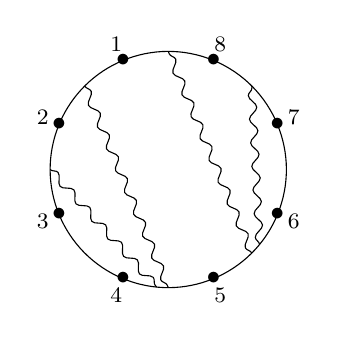
\begin{tikzpicture}[rotate=67.5,baseline=(current bounding box.east)]
	\begin{scope}
	\drawWLD{8}{1.5}
	\drawnumbers
	\drawprop{1}{0}{4}{0}
	\drawprop{2}{0}{4}{-1}
    \drawprop{5}{0}{8}{0}
    \drawprop{5}{1}{7}{0}
		\end{scope}
	\end{tikzpicture}\]

\caption{The Wilson loop diagram $W = \big(\{(1,4), (2,4), (5,7), (5,8)\},[8]\big)$ which has four propagators and eight vertices.}
\label{fig:ex of WLD}
\end{figure}

Let $[n]$ denote the set of integers $\{1,\dots,n\}$ with the obvious cyclic and linear orders. Our primary focus is Wilson loop diagrams with $V = [n]$, so in order to simplify the exposition we will often use $i+1$ as shorthand for ``the successor of vertex $i$''. 

Generally speaking the propagators in a Wilson loop diagram are undirected, so $(i,j)$ and $(j,i)$ represent the same propagator. If we need to impose a direction on a propagator $p = (i,j)$, for example in order to consider the region ``inside'' or ``outside'' of $p$, we write $(p,<_i)$ to indicate that $p$ is directed from edge $i$ to edge $j$, and $(p,<_j)$ for the opposite direction.

We also impose the convention that all vertices should always be interpreted in terms of the cyclic order on $V$; for example, if $V = [n]$ then $(n,n+3)$ means the propagator connecting edges $3$ and $n$. This viewpoint is beneficial for us since many of our proofs rely on restricting our attention to a region of the diagram bounded by a given propagator, or to short propagators such as $(i,i+2)$, and these behave the same regardless of whether we cross the ``first'' vertex or not; however, we emphasize that this is different to the standard convention in the physics literature, where propagators are written $(i,j)$ with $1 \leq i<j \leq n$.



\begin{dfn} \label{VPropdfn}
Let $W = (\cP, V)$ be a Wilson loop diagram.
\begin{enumerate}
\item For $p = (i,j) \in \cP$, let $V(p) = \{i, i+1, j, j+1\}$ denote the set of {\bf vertices supporting $p$}. For a set of propagators $P \subseteq \cP$, define 
\[V(P) = \bigcup_{p \in P} V(p)\]
to be the vertex support of $P$.
\item For $U \subseteq V$, the set of {\bf propagators supported on $U$} is denoted by
\[\Prop(U) = \{ p \in \cP\ |\ V(p) \cap U \neq \emptyset \}.\]
Note that a propagator in $\Prop(U)$ does not need to have its entire support contained in $U$. 
\item Vertices of $W$ that do not support any propagators are called {\bf non-supporting}. The set of all non-supporting vertices in $W$ is denoted $F(\emptyset)$. 
\end{enumerate}
\end{dfn}

In particular, we will see in later sections that all four vertices in the support of a propagator are important in understanding the contribution of that propagator to the overall diagram. This motivates the following definition of a subdiagram, which can consist of any subset $Q$ of the propagators and any subset $U$ of the vertices of $W$ {\em as long as we retain all vertices in the support of $Q$}.

\begin{dfn} \label{subdiagramdfn}
Let $W = (\cP, V)$ be a Wilson loop diagram. Then $W' = (Q,U)$ is a {\bf subdiagram} of $W$ if $Q \subseteq \cP$ and $V(Q) \subseteq U \subseteq V$.
\end{dfn}



With these definitions in hand, we can impose some conditions on the density and behavior of the propagators of Wilson loop diagrams.

\begin{dfn}\label{admisdfn}
A Wilson loop diagram $W = (\cP, V)$ is called {\bf admissible} if:
\begin{enumerate}
\item $|V| \geq |\cP| + 4$.
\item There does not exist a non-empty set of propagators $Q \subseteq \cP$ such that $|V(Q)| < |Q| + 3$.
\item There does not exist a pair of propagators $\{(i,j),(k,l)\} \subseteq \cP$ such that $i < k < j < l$.
\end{enumerate}
 \end{dfn}

The first condition bounds the total number of propagators in the diagram, while the second limits how densely propagators can be fitted into any part of the diagram; in particular, it prohibits propagators that connect two adjacent edges and parallel propagators that start and end on the same pair of edges. The third condition simply requires that propagators are non-crossing. 

These conditions are imposed by the physical interpretation of Wilson loop diagrams (see for example \cite{Adamo:2011pv,Adamo:2012xe,wilsonloop,LipsteinMason}). We therefore restrict our attention in this paper to admissible Wilson loop diagrams and their subdiagrams only. 

Note that a subdiagram $(Q,U)$ of an admissible Wilson loop diagram need not be admissible itself: it inherits conditions 2 and 3 automatically, but we could have $|U| = |Q| + 3$. If a Wilson loop diagrams satisfies conditions 2 and 3 of Definition~\ref{admisdfn}, we call it {\bf weakly admissible}.

These diagrams correspond to (tree level) amplitudes of SYM $N=4$ theory in twistor space. As such, it associates a real value to $n$ particles, one for each vertex. Each particle is represented as a section of a $|\cP|$-vector bundle over twistor space, projected onto a real subspace in a process called bosonization \cite{Arkani-Hamed:2013jha}. In other words, each Wilson loop diagram defines a functional on external particles. This is represented as an integral $I(W)$, which is the equivalent of a Feynman integral in this setting. 

A $|\cP| \times n$ matrix $C(W)$ represents the (tree level) particle interactions. Each row of $C(W)$ corresponds to an internal propagator, each column to an external particle. $C(W)$ is defined as follows:

\begin{equation} C(W)_{p,q} = \begin{cases} c_{p,q} & \textrm{ if } q \in V(p) \\
0  & \textrm{ if } q \not \in V(p)  \end{cases}
\;. \label{C(W) dfn}\end{equation} \todo{$c_{p,q}$ or $x_{p,q}$? Should be consistent} 

The entries $c_{p,q}$ are non-zero real variables. Thus the zero entries in row $p$ correspond to the external particles that the propagator $p$ does not interact with. See \ref{integraldetails} for an example of a diagram $W$ and its associated matrix.

The matrix $C(W)$ can be interpreted as a parametrization of the positroid cell in the positive Grassmannian $\Gr(n, |\cP|)$ associated to the $W$, which we denote by $\Sigma(W)$ \cite{wilsonloop}. Most of the work in this paper, and in \cite{generalcombinatoricsI} focuses on characterizing the positroid cell assoicated to eash Wilson loop diagram $W$. 

Note that since there is no ordering on the propagators of $W$, $C(W)$ is only defined up to rearrangement of the rows. This will not matter here, as it does not affect the parametrization of $\Sigma(W)$.

One may also interpret the functional $I(W)$ as associating a volume to each cell $\Sigma(W)$ \cite{wilsonloop, Amplituhedronsquared, HeslopStewart}. The volume form is written in terms of the elements of $C(W)$ as  \[ \Omega(W) = \frac{\prod_{r=1}^{|\cP|} \prod_{v \in V_{p_r}} \textrm{d}c_{p_r}}{R(W)} \;. \]
The interested reader is referred to \cite{Adamo:2012xe,HeslopStewart,LipsteinMason} for more information about the volume form. 

For a fixed number of propagators and particles, the tree level amplitude of the Wilson loop diagrams is computed as the sum of the $I(W)$ for all $W$ of the correct size. By \cite{Adamo:2011pv,Adamo:2012xe,Arkani-Hamed:2013jha} this sum is finite for all sets of external particles, i.e. we have \bas \mathcal{A}_{k, n}^{tree} = \sum_{(\cP, [n]), |\cP| = k} I(W) <\infty. \eas

In particular, this implies that any singularities in the integrals $I(W)$ must cancel out in the sum. In particular, they must cancel on the boundaries of the positroid cells $\Sigma(W)$, analogous to the analysis in \cite{Arkani-Hamed:2013jha}. This has been checked for particular classes of examples (e.g. \cite{casestudy, Amplituhedronsquared, HeslopStewart}) but has not been proven in general.

With this motivation in mind, in this paper we study the denominator $R(W)$ of the volume form $\Omega(W)$, which we define next.

\begin{dfn}\label{def R(W)}
Let $W = (\cP,V)$ be an admissible Wilson loop diagram, and fix an edge $e$. Let $\{p_1 \ldots p_r\}$ be the propagators with one end lying on edge $e$, ordered so that $p_1$ is closest to the vertex $e$, $p_r$ closest to $e+1$, and $p_i$ is closer to $e$ than $p_{i+1}$ is. Define 
\[ R_e =  c_{p_1,e+1} \prod_{j= 1}^{r-1} \left((c_{p_j,e} c_{p_{j+1},e+1} - c_{p_{j+1},e} c_{p_{j},e+1} ) \right) c_{p_r,e}\;\]
to be the component of $R(W)$ associated to edge $e$. Note that if $r = 1$ (i.e. there is exactly one propagator lying on edge $e$) then this expression simplifies to $R_e = c_{p,e} c_{p,e+1}$. If $r=0$, set $R_e = 1$. The denominator $R(W)$ is defined to be the product of all of the $R_e$, i.e. 
\[R(W) = \prod_{e \in V} R_e.\]
\end{dfn}

In Section \ref{sec poles}, we show that the denominator $R(W)$ is determined by the positroid cell $\Sigma(W)$ and the structure of $W$, as encapsulated by $C(W)$. In fact, it can be read directly off of $C(W)$, in terms of characterization of $\Sigma(W)$ called the Grassmann necklace (see Definition~\ref{def:grassmann necklace}). We also give an algorithm to read $R(W)$ directly from the Wilson loop diagram, paving the way for a general study of these poles in future.

We end this section with an example of computing $C(W)$ and $R(W)$ for a particular Wilson loop diagram $W$.

\begin{eg} \label{integraldetails}
Consider the admissible Wilson loop diagram 
\[W = \big(\{(1,4), (2,4), (5,7), (5,8)\},[8]\big),\]
from Figure~\ref{fig:ex of WLD}. Ordering the propagators as listed above, we obtain the associated matrix
\[ C(W) = \left(
\begin{array}{cccccccc}
c_{1,1} & c_{1,2} & 0 & c_{1,4} & c_{1,5} & 0 & 0 & 0 \\
0 & c_{2,2} & c_{2,3} & c_{2,4} & c_{2,5} & 0 & 0 & 0 \\
0 & 0 & 0 & 0 & c_{3,5} & c_{3,6} & c_{3,7} & c_{3,8} \\
c_{4,1} & 0 & 0 & 0 & c_{4,5} & c_{4,6} & 0 & c_{4,8}  \\
\end{array}
\right) \;.\]

To calculate $R(W)$, write \bmls R_1 = c_{1,1} c_{1, 2}\quad R_2 = c_{2,2} c_{2,3} \quad R_4 = c_{2,5} (c_{2,4}c_{1,5} - c_{2,5}c_{1,4})c_{1,4} \\ R_5 = c_{4,6} (c_{4,6}c_{3,5} - c_{3,6}c_{4,5})c_{3,5} \quad R_7 = c_{3,7} c_{3,8} \quad R_8 = c_{4,8} c_{4,1} \;.\emls All other $R_e$ are $1$.  Finally, the integrand associated to this Wilson loop diagram is \bas \Omega(W) = \frac{\textrm{d}c_{1,1}\textrm{d}c_{1,1}\textrm{d}c_{1,1}\textrm{d}c_{1,2}\textrm{d}c_{1,4}\textrm{d}c_{1,5}\textrm{d}c_{2,1}\textrm{d}c_{2,3}\textrm{d}c_{2,4}\textrm{d}c_{2,5}\textrm{d}c_{3,5}\textrm{d}c_{3,6}\textrm{d}c_{3,7}\textrm{d}c_{3,7}\textrm{d}c_{4,5}\textrm{d}c_{4,6}\textrm{d}c_{4,8}\textrm{d}c_{4,1}}{c_{1,1} c_{1, 2}c_{2,2} c_{2,3}c_{2,5} (c_{2,4}c_{1,5} - c_{2,5}c_{1,4})c_{1,4}c_{4,6} (c_{4,6}c_{3,5} - c_{3,6}c_{4,5})c_{3,5}c_{3,7} c_{3,8}c_{4,8} c_{4,1}} \;. \eas
\note{Is the numerator just supposed to be the product of $dc_{pq}$ for each $c_{pq}$ in the matrix? Also I think $c_{46}c_{35} - c_{36}c_{45}$ in the denominator is the wrong way around?}
\end{eg}



\subsection{Positroids, Grassmann necklaces, and Le diagrams}\label{sec:positroid background}

We summarize here only the subset of positroid theory that we require in this paper; the interested reader is referred to \cite{Postnikov} for more details. 

Let $\binom{[n]}{k}$ denote the set of all $k$-subsets of $[n]$.  

For our purposes, a {\bf positroid} is a matroid $M$ (with ground set $[n]$ and bases $\cB \subseteq \binom{[n]}{k}$) which can be represented by an element of the positive Grassmannian $\Gr(k,n)$. In other words, there exists a full-rank $k\times n$ real matrix whose $k\times k$ minors are all nonnegative and such that the minor $[[k]|J]$ is positive if and only if $J \in \cB$.

Postnikov shows in \cite{Postnikov} that the positroids of $\Gr(k,n)$ are indexed by many different collections of objects, each with their own advantages and disadvantages. The two most suited to our purposes are Grassmann necklaces and Le diagrams, which we introduce below. In order to do so, we first need some preliminary definitions.

For each $j \in [n]$, we can define a total order $<_j$ on the interval $[n]$ by
\[ j <_j j+1 <_j \dots <_j n <_j 1 \dots <_j j-1\;.\]
This in turn induces a total order on $\binom{[n]}{k}$, namely the lexicographic order with respect to $<_j$.  It also induces a separate partial order $\gale{j}$ on $\binom{[n]}{k}$ (the {\bf Gale order} \cite{Gale}), which is defined as follows: for 
\[A = \{a_1 <_j a_2 <_j \dots <_j a_k\} \text{ and } B = \{b_1 <_j b_2 <_j \dots <_j b_k\} \in \binom{[n]}{k},\] we define
\[A \gale{j} B \text{ if and only if } a_r \leq_j b_r \text{ for all }1 \leq r \leq k.\]
For example, in $\binom{[6]}{3}$ we have $\{2,5,6\}\gale{2} \{2,6,1\}$ but $\{2,5,6\}\not\gale{2}\{3,4,6\}$.


\begin{dfn}\label{def:grassmann necklace}
A {\bf Grassmann necklace} of type $(k,n)$ is a sequence $(I_1, \dots, I_n)$ of $n$ sets $I_i \in \binom{[n]}{k}$ such that for each $i \in [n]$:
\begin{itemize}
\item if $i \in I_i$, then $I_{i+1} = \big(I_i \backslash \{i\}\big) \cup \{j\}$ for some $j \in[n]$.
\item if $i \not\in I_i$, then $I_{i+1} = I_i$.
\end{itemize}
By convention, we set $I_{n+1} = I_1$.
\end{dfn}

By \cite[Theorem 17.1]{Postnikov}, the Grassmann necklaces of type $(k,n)$ are in 1-1 correspondence with the positroid cells in $\Gr(k,n)$. Each term $I_i$ is simply the minimal (with respect to the $<_i$-lex order) basis of the positroid. A characterization of all bases of the positroid in terms of the Grassmann necklace and the Gale order was given by Oh in \cite[Theorem 8]{Oh}: if $(I_1, \dots, I_n)$ is the Grassmann necklace associated to a positroid $M = ([n],\cB)$, then the bases of $M$ are exactly
\ba \cB = \left\{J \in \binom{[n]}{k}\ |\ I_i \gale{i} J \ \forall i \in [n]\right\}. \label{basesofmatroids}\ea
Thus the Grassmann necklace is well suited to testing whether a given $k$-set is a basis for $M$, and for generating a list of all bases of $M$.


\begin{dfn}\label{def:le diagram}
A {\bf Le diagram} is a Young diagram in which every square contains either a $+$ or a $0$, subject to the rule that if a square contains a $0$ then either all squares to its left (in the same row) must also contain a $0$, or all squares above it (in the same column) mustbasesofmatroids\ also contain a $0$, or both.
\end{dfn}

By \cite[Theorem 6.5]{Postnikov}, the set of all Le diagrams that fit within a $k\times(n-k)$ rectangle is in 1-1 correspondence with the positroid cells of $\Gr(k,n)$. Le diagrams are particularly useful for comparing dimensions of positroids, since the dimension of a positroid is equal to the number of $+$ squares in its Le diagram \cite[Theorem 6.5]{Postnikov}.

The rows and columns of a Le diagram are labelled as follows: given a Le diagram fitting inside a $k\times (n-k)$ box, arrange the numbers $1,2, \dots, n$ along its southeast border, starting from the top-right corner. See Figure \ref{fig:row column numbering} for examples.

\begin{figure}[h!]
\[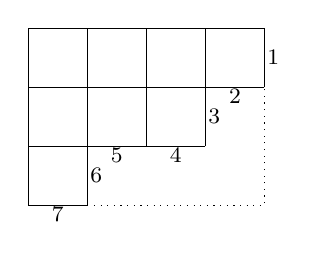
\begin{tikzpicture}[baseline=(current bounding box.east),scale=0.75]
\draw (1,0) grid (2,3);
\draw (2,1) grid (4,3);
\draw (4,2) grid (5,3);
\draw[dotted] (2,0) -- (5,0) -- (5,2);

\node at (5.15,2.5) {\footnotesize$1$};
\node at (4.5,1.85) {\footnotesize$2$};
\node at (4.15,1.5) {\footnotesize$3$};
\node at (3.5,0.85) {\footnotesize$4$};
\node at (2.5,0.85) {\footnotesize$5$};
\node at (2.15,0.5) {\footnotesize$6$};
\node at (1.5,-0.15) {\footnotesize$7$};
%\node at (0.5,-0.15) {\footnotesize$8$};
\end{tikzpicture}
\qquad \qquad
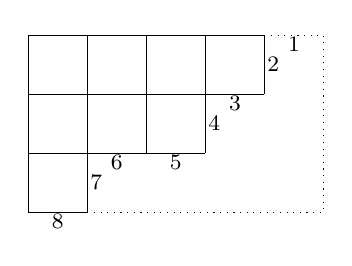
\begin{tikzpicture}[baseline=(current bounding box.east),scale=0.75]
\draw (1,0) grid (2,3);
\draw (2,1) grid (4,3);
\draw (4,2) grid (5,3);
\draw[dotted] (2,0) -- (6,0) -- (6,3) -- (5,3);

\node at (5.5,2.85) {\footnotesize$1$};
\node at (5.15,2.5) {\footnotesize$2$};
\node at (4.5,1.85) {\footnotesize$3$};
\node at (4.15,1.5) {\footnotesize$4$};
\node at (3.5,0.85) {\footnotesize$5$};
\node at (2.5,0.85) {\footnotesize$6$};
\node at (2.15,0.5) {\footnotesize$7$};
\node at (1.5,-0.15) {\footnotesize$8$};
%\node at (0.5,-0.15) {\footnotesize$9$};
\end{tikzpicture}
\]
\caption{Row and column numbering for a Young diagram with $k = 3$, $n = 7$ (left) and $k = 3$, $n = 8$ (right). The top left box has coordinates $(1,7)$ in the left diagram, and $(2,8)$ in the right diagram.}
\label{fig:row column numbering}
\end{figure}

Specifying a $k$-subset $J \subseteq [n]$ therefore uniquely determines the shape of the Le diagram, by taking the elements of $J$ to be the row indices of the diagram.

An algorithm for constructing the Le diagram associated to a Grassmann necklace was given by Agarwala and Fryer in \cite{reversingOh}. Since we will make use of this algorithm in Section~\ref{sec dim} below, we summarize the process here.
\begin{algorithm}\label{alg:GN to Le} \ \cite[Algorithm 2]{reversingOh}
Let $(I_1,\dots,I_n)$ be a Grassmann necklace of type $(k,n)$. Within a $k \times(n-k)$ square, draw the Young diagram whose rows are labelled by $I_1$ (as per the convention above).

For each $i$, $2 \leq i \leq n$:
\begin{itemize}
\item Write \[I_1 \setminus I_i = \{a_1 > a_2 > \dots > a_r\}, \quad I_i \setminus I_1 = \{b_1 < b_2 < \dots < b_r\},\]
where the inequalities denote the $<_1$ order (subscripts suppressed for clarity).
\item For $1 \leq j \leq r$ , place a $+$ in square $(a_j,b_j)$ of the diagram. (We will sometimes refer to this $+$ as being {\em in the $a_j \rightarrow b_j$ position}.)
\end{itemize}
After performing the above for $2 \leq i \leq n$, place a $0$ in any remaining unfilled boxes.
\end{algorithm}

An algorithm for constructing the Grassmann necklace of a Le diagram also exists; this was given by Oh in \cite{Oh}. A method for using the Le diagram to test whether a given $k$-subset is a basis for the corresponding positroid or not was given by Casteels in \cite{CasteelsPaths}.



\subsection{Wilson loop diagrams as positroids}\label{sec:WLD as positroids}


Let $W = (\cP,[n])$ be an admissible Wilson loop diagram with $k$ propagators, and $C(W)$ the associated matrix defined in \eqref{C(W) dfn}. Let $M(W)$ be the matroid realized by $C(W)$, i.e. the matroid with ground set $[n]$ whose independent sets are exactly the sets $V \subseteq [n]$ such that the columns of $C(W)$ indexed by $V$ are linearly independent.

In \cite{wilsonloop}, Agarwala and Amat show that $M(W)$ is also characterized by the Wilson loop diagram itself:

\begin{thm} \label{thm WLD defines matroid} \cite[Theorem 3.6]{wilsonloop} The independent sets of the matroid $M(W)$ associated to an admissible Wilson loop diagram $W = (\cP,[n])$ and realized by $C(W)$ are exactly those subsets $V \subseteq [n]$ such that $\nexists U\subseteq V$ satisfying $|\Prop(U)| < |U|$. \end{thm}
In other words, the independent sets of $M(W)$ correspond to sets of vertices in $W$ in which no subset supports fewer propagators than the vertices it contains.

One useful corollary of this, which we will want to keep in mind later, is the following.
\begin{cor}\label{lem basis as perm}
Let $W = (\cP,[n])$ be an admissible Wilson loop diagram and let $M(W)$ be its associated matroid. A subset $J \subseteq [n]$ is an independent set of $M(W)$ if and only if there exists an injective set map $f : J \rightarrow \cP$ with the property that for each $j\in J$ we have $j \in V(f(j))$.
\end{cor}

\begin{proof}
  This follows as a corollary of the previous theorem by induction in one direction and the pigeonhole principle in the other direction.  

Forgetting about the matroid and simply thinking about the condition of linear independence in the matrix $C(W)$, the corollary can also be proved directly by linear algebra and the definition of $C(W)$ as follows: because the nonzero entries of $C(W)$ are independent indeterminants, $J$ is an independent set is if and only if there is some choice of $|J|$ nonzero entries of $C(W)$ one in each row associated to an element of $J$ and each in different columns. Each entry in $C(W)$ identifies a propagator by the row of the entry and a vertex by the column of the entry.  The entry is nonzero if and only if the propagator is supported on that vertex.  Consequently, a choice of $|J|$ nonzero entries of $C(W)$ one in each row associated to an element of $J$ and each in different columns is equivalent to an assignment of the propagators of $J$ to supporting vertices so that no two are assigned to the same vertex.  Such an assignment of the propagators of $J$ to supporting vertices is exactly a map $f$ as described in the statment, hence proving the result.
\end{proof}

In particular, this corollary says that a subset $J$ of $[n]$ is a basis of $M(W)$ if and only if there is a set bijection between $J$ and $\cP$ with the property that for each $j\in J$ the propagator associated to $j$ under the bijection is supported on vertex $j$.


By relating the behavior of the propagators in $W$ to the matroidal properties of $M(W)$, Agarwala and Amat also showed that $M(W)$ is in fact a positroid whenever $W$ is admissible \cite[Corollary 3.39]{wilsonloop}.

However, in order to identify the positroid associated to a given Wilson loop diagram $W$ we first have to construct $C(W)$, then make a list of all its non-zero $k\times k$ minors and extract the Le diagram or Grassmann necklace via the methods described in Section~\ref{sec:positroid background}. Alternatively, one could obtain the decorated permutation of the positroid from $C(W)$ as in \hlfix{[ref]}{Sian needs to go find this reference} and then convert it into a Grassmann necklace as described in \cite[Section 16]{Postnikov}. 

In \cite{casestudy}, Agarwala and Fryer apply this process in the smallest non-trivial case: admissible Wilson loop diagrams with two propagators on six vertices. Even in this simple case, we see that the mapping from admissible WLD to positroid cells is neither one-to-one nor onto, and the process described above makes it almost impossible to track the relationship between the original Wilson loop diagram and the resulting positroid.

Our first goal is therefore to find a better method of obtaining the positroid associated to a given Wilson loop diagram; this is the focus of the next section.

\begin{rmk}
While this paper primarily approaches proofs from a combinatorial point of view, readers with a background in matroid theory are encouraged to keep the matroidal viewpoint in mind throughout; we expect that the two approaches will be complementary and will build upon each other. See \cite{generalcombinatoricsI} for some related results concerning the positroids of Wilson loop diagrams obtained by viewing them primarily as matroids.
\end{rmk}




\section{Wilson Loop diagrams and their Grassmann necklaces}\label{sec GN algorithm}



In this section we will give an algorithm (Algorithm~\ref{alg:put GN on WLD}) to go directly from a Wilson loop diagram to the Grassmann necklace of its positroid. This is a useful result in and of itself, as it greatly simplifies the process of identifying the positroid associated to a given WLD. It also allows us to examine how the positroid changes as we make minor changes to the Wilson loop diagram; indeed, the techniques we develop in this section to verify that our algorithm produces the correct Grassmann necklace will also be used repeatedly in later sections.

One of the key insights is that each element of the Grassmann necklace can be viewed as a function from the propagators of the diagram to the vertices in the Grassmann necklace element.  This is captured in Definition~\ref{def I_i as a function}, and used throughout the paper.


%\note{Sian thinks that a section roadmap here would be overkill: we gave a roadmap in section 1, each subsection has its own little intro roadmap, and I've added a ref to the algorithm above so that people can skip straight to it if they want}

%In Section~\ref{sec:propagator configs} we examine the structure of admissible Wilson loop diagrams and prove several technical lemmas about configurations of propagators appearing in these diagrams. In Section~\ref{sec:GN alg} we state the algorithm that extracts the Grassmann necklace of a given diagram (see Algorithm~\ref{alg:put GN on WLD}) and 

Throughout this section, $W = (\cP,[n])$ is an admissible Wilson loop diagram with $k$ propagators.





\subsection{Propagator configurations in admissible Wilson loop diagrams}\label{sec:propagator configs}

Before we can describe the algorithm for extracting the Grassmann necklace of $M(W)$ from the Wilson loop diagram $W$, we require some initial results about the behavior of propagators in admissible WLD.



\begin{dfn}\label{props inside p}
Let $W = (\cP, [n])$ be a weakly admissible Wilson loop diagram, with $p \in \cP$ supported on edges $i$ and $j$. Write $(p, <_i)$ to represent the same propagator directed from $i$ to $j$. Then the sets of propagators {\bf inside} and {\bf outside} of $(p,<_i)$ are defined to be
\begin{gather*}\cP_{in}(p,<_i) = \{ (k,l) \in \cP \ |\ i \leq_i k <_i l \leq_i j \}, \\
\cP_{out}(p,<_i) = \cP\setminus \cP_{in}(p,<_i),
\end{gather*}
respectively.
\end{dfn}


\begin{eg}
Let $W$ be the Wilson loop diagram from Figure \ref{fig:ex of WLD}, reproduced here for convenience.  \[W\ =\ 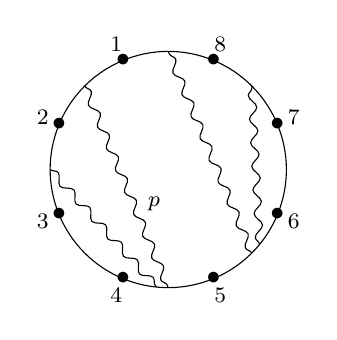
\begin{tikzpicture}[rotate=67.5,baseline=(current bounding box.east)]
	\begin{scope}
	\drawWLD{8}{1.5}
	\drawnumbers
	\drawlabeledprop{1}{0}{4}{0}{\footnotesize \qquad \ $p$}
	\drawprop{2}{0}{4}{-1}
    \drawprop{5}{0}{8}{0}
    \drawprop{5}{1}{7}{0}
		\end{scope}
	\end{tikzpicture}\]

Let $p$ be the propatagor $p = (1, 4)$. Then $\cP_{in}(p, <_4) = \{(1,4), (5, 8), (5, 7) \}$ and $\cP_{out}(p, <_4) = \{(2,4) \}$
\end{eg}


\begin{dfn}
Let $p = (i,j) \in \cP$ be a propagator in $W$.  Define the {\bf length} of $p$ to be 
\[\ell(p) \  =\ \min\big\{|[i+1,j]|,|[j+1,i]|\big\}.\]
\end{dfn}
In other words, $\ell(p)$ is the size of the smaller of the sets of vertices on either side of the propagator $p$.


\begin{rmk}\label{rem:props of length 2 and 3} 
The following observations about configurations of propagators of short length in a weakly admissibly Wilson loop diagram $W$ are easily verified:
\begin{enumerate}
\item If $p = (i,i+3)$ is a propagator of length 3, then the middle vertex $i+2$ supports at most one propagator.
\item If every vertex in $W$ supports at least one propagator, then $W$ admits at least one propagator of length 2.
\end{enumerate}
\end{rmk}


The following lemma establishes certain configurations of propagators that must exist in any admissible diagram with no non-supporting vertices (i.e. with $F(\emptyset) = \emptyset$). We make use of this result in several induction proofs below. 

\begin{lem}\label{lem sian}
  Let $W$ be a weakly admissible WLD with at least 5 vertices and in which each vertex supports at least one propagator.  Then at least one of the following two things occurs.
  \begin{enumerate}
    \item $W$ has a propagator of length $\leq 6$ with a propagator of length 2 on one side it and nothing else on that side.\label{item big and 2}
    \item There exists a pair of propagators of length $2$ with the property that the first propagator is $(i, i+2)$, the second is $(j, j+2)$, no other propagator ends between vertices $i+2$ and $j+1$, and $j\in\{i+2, i+3, i+4\}$.\label{item pair of 2s}
  \end{enumerate}
\end{lem}

\begin{proof}
Suppose first that $W$ has a propagator of length $3$, say $p=(i, i+3)$.  By Remark~\ref{rem:props of length 2 and 3} and the fact that every vertex of $W$ supports at least one propagator, we have that $i+2$ supports exactly one propagator and this propagator must have length 2 by noncrossingness.  This gives us an instance of configuration~\ref{item big and 2} from the statement.

Now suppose $W$ has no propagators of length $3$.
  
We will inductively construct a sequence of propagators $p_r$ and $q_r$, with $\ell(p_r) = 2$ for each $r$ and either:
\begin{itemize}
\item $p_r$ forms part of configuration \ref{item big and 2} or \ref{item pair of 2s} from the statement, at which point the induction terminates, 
  %a configuration \eqref{eq:2 prop config} in $D$
{\em or} 
\item there is a propagator $q_r$ satisfying $\ell(q_r) \geq 4$, and $\{p_1, \ldots, p_r, q_1, \ldots, q_{r-1}\}$ are all on the same side of $q_r$.  
\end{itemize}
We can then choose the orientation of $q_r$ so that the previous $p_i$ and $q_i$ are all on the outside of $q_r$, and restrict our attention to the subdiagram $(\cP_{in}(q_r),[n])$. By the finiteness of $W$ this must eventually terminate in one of the desired configurations. %a configuration of the form \eqref{eq:2 prop config}.

Start by choosing a propagator $p_1 = (j_1,j_1+2)$ of length 2 in $W$ (which exists by Remark~\ref{rem:props of length 2 and 3}).  If it is part of one of the configurations we are looking for then we are done, 
%a configuration \eqref{eq:2 prop config} we are done,
so suppose otherwise. 

From our existing assumptions, we know the following facts: $p_1$ is not in configuration \ref{item pair of 2s}, there are no propagators of length $3$, and every vertex supports at least one propagator.  Therefore there must be a propagator of length $\geq 4$ with one end on edge $j_1$ or on edge $j_1-1$ or on edge $j_1-2$.  Let $q_1 = (i_1, k_1)$ be this propagator, oriented such that $p_1 \in \cP_{out}(q_1,<_{i_1})$. This completes the base case.

\bas 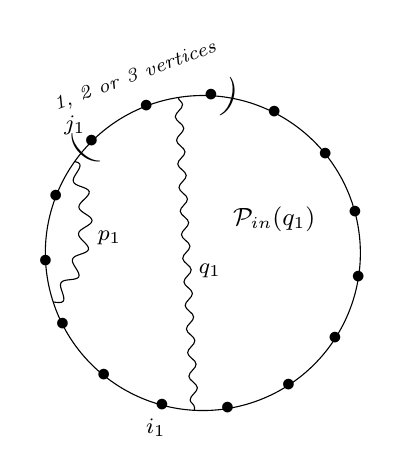
\begin{tikzpicture}[rotate=15,baseline=(current bounding box.east)]
	\begin{scope}
	\drawWLD{15}{2}
	%\drawnumbers
	%\drawprop{1}{0}{4}{0}
	\begin{scope}
	\clip (0,0) circle (\radius cm);
	\draw[propagator] (\angle*5.3:\radius*1.2cm) to [bend left=50] (\angle*7.7:\radius*1.2cm);
	\node at (\angle*6.5:\radius*0.6cm) {\footnotesize $p_1$};
	\end{scope}
    \drawlabeledprop{3}{0}{10}{0}{\footnotesize \qquad $q_1$};
    \node at (\angle*5:\radius*1.15cm) {\footnotesize $j_1$};
     \node at (\angle*10:\radius*1.15cm) {\footnotesize $i_1$};
     \node at (10:\radius*0.5) {\small $\cP_{in}(q_1)$};
	\node[rotate = 45] at (\angle * 5.2:\radius) {\Large $($};
\node[rotate = -15] at (\angle * 2.7:\radius) {\Large $)$};
\node[rotate = 20] at (\angle* 4:\radius*1.2) {\em \scriptsize 1, 2 or 3 vertices};
		\end{scope}
	\end{tikzpicture}\eas 

 %\node[rotate=-15] at (\zero + 2.7*\step:\radius) {\Large $($};
 %    \node[rotate=15] at (\zero + 6.3*\step:\radius) {\Large $)$};
   %  \node at (\zero + 4.5*\step:\radius*0.85) {\em \scriptsize up to 4 vertices here};

\sanote{played with Sian's code. May need to tweak this picture}
Now suppose $q_{r} = (i_r, k_r)$ exists by the induction hypothesis and is oriented $(q_r, <_{i_r})$ so that the previous $p_i$ and $q_i$ are on the outside. For the rest of this proof, we assume this orientation and drop the $<_{i_r}$ from the notation.

Let $W_r := (\cP_{in}(q_r),[n])$ be the subdiagram of $W$ consisting only of those propagators inside $q_r$ (including $q_r$ itself); in particular $W_r$ contains none of the previous $p_i$ or $q_i$. By the original hypotheses on $W$, every vertex in $[i_r,k_{r+1}]$ (of which there are at least 4, since $\ell(q_r) \geq 4$) must support at least one propagator. Therefore $W_r$ admits at least one propagator of length 2 (by Remark~\ref{rem:props of length 2 and 3}) and no propagators of length $3$ (by our assumption on $W$).

Let $p_{r+1} = (j_{r+1}, j_{r+1}+2)$ be a propagator of length 2 in $W_r$; if it forms part of configuration \ref{item big and 2} or \ref{item pair of 2s}
%the configuration \eqref{eq:2 prop config}
then we are done, so assume otherwise. 

Note that we could replace $q_r$ by another propagator $q'_{r}$ in $W_r$, as long as $p_{r+1}$ and $q_r$ are on opposite sides of $q_r'$: such a new $q'_{r}$ would still satisfy all of the induction hypotheses. Therefore without loss of generality we may assume that $\cP_{in}(q_r)$ does not contain any propagators (other than $q_r$ itself) which satisfy the induction hypotheses, i.e. we assume that there are no other propagators with $p_{r+1}$ on one side and $q_r$ on the other.

There are two cases to consider.

The first case is that $i_r \leq j_{r+1} \leq i_r+2$ and $k_r-2 \leq j_{r+1}+2 \leq k_{r}$ (so $p_{r+1}$ has one end before $i_{r} + 3$ and the other after $k_{r} - 2$, i.e. both ends of $p_{r+1}$ are close to the ends of $q_r$).  Then since $p_{r+1}$ has length 2, it must be that $(i_r+3)+1 \geq k_r-2$ and so $q_r$ has length $\leq 6$.  By the minimality assumption on $q_r$, no propagator in $W_r$ has $q_r$ on one side and $p_{r+1}$ on the other side. Therefore, any propagator in $W_r$ other than $q_r$ and $p_{r+1}$ must be of the form $(i,j)$ with $i_r\leq i < j\leq i_r+2$ or $k_r-2 \leq i < j\leq k_r$. Both of these require that $(i,j)$ has length 2, and so we have configuration \ref{item pair of 2s} which we have already assumed does not occur.  Consequently, $W_r$ contains only the two propagators $q_r$ and $p_{r+1}$, yielding configuration \ref{item big and 2} from the lemma statement and again contradicting our assumption. Therefore this first case cannot occur.

The second case is that (at least) one of the following four things happen:
\begin{itemize}
\item $i_r+3 \leq j_{r+1}\leq k_r-3$, or
\item $i_r+3 \leq j_{r+1}+2\leq k_r-3$, or
\item $i_r = j_{r+1}$, or 
\item $k_r-2 = j_{r+1}$
\end{itemize}
In other words, at least one end of $p_{r+1}$ is supported entirely by vertices in the interval $[i_r+3,k_r+2]$ (the first two bullet points) or both ends lie in $[i_r, i_r+3]$ (third point) or both ends lie in $[k_r-2, k_r+1]$ (fourth point). These situations all behave similarly, and by symmetry it suffices to only consider the second and third possibilities. 

Note that since $j_{r+1}+4 \leq k_r-1$ in both of these situations, the vertex $j_{r+1}+4$ is inside $q_r$ but does not support either $q_r$ or $p_{r+1}$, and must therefore support some other propagator $t$.  Since $p_{r+1}$ is not part of configuration \ref{item pair of 2s} and $W_r$ has no propagators of length 3, it follows that $\ell(t) \geq 4$.  If $q_r$ and $p_{r+1}$ were on different sides of $t$ then this would contradict the minimality of $q_r$.  Therefore we can orient $t$ so that all previous $q_i$ and $p_i$ belong to $\cP_{out}(t)$, and set $q_{r+1} = t$ to continue the induction.

The overall result then follows by induction.
\end{proof}

\begin{rmk}
In the case that all vertices of an admissible WLD $W$ support at least two propagators, then Lemma~\ref{lem sian} substantially simplifies.  By Remark~\ref{rem:props of length 2 and 3}, $W$ has no propagators of length $3$.  Configuration \ref{item big and 2} necessarily entails vertices with support $1$ as does configuration \ref{item pair of 2s} unless $j=i+2$.  So in the case that $W$ has all vertices with support at least two then $W$ must contain a pair of propagators of length $2$  with the property that the first propagator is $(i, i+2)$, the second is $(i+2, i+4)$ and no other propagator ends on the edge $i+2$.
\end{rmk}


\subsection{From Wilson Loop diagrams to Grassmann Necklaces}\label{sec:GN alg}

Until now, the positroid associated to a Wilson loop diagram $W$ could only be obtained by computing the matrix $C(W)$ associated to $W$, listing all bases of the induced matroid $M(W)$, and constructing the Le diagram or Grassmann necklace of the positroid ``by eye'' from this list. 

In this section, we give an algorithm for passing directly from the Wilson loop diagrams to its Grassmann necklace. This not only greatly simplifies the process above, but will also allow us to relate the behavior of the positroid $M(W)$ directly to the configuration of progators in $W$.

The fact that Algorithm~\ref{alg:put GN on WLD} does construct the required Grassmann necklace is proved in Theorem~\ref{res:alg gives GN}. An worked example of Algorithm~\ref{alg:put GN on WLD} is given in Example~\ref{eg:apply GN alg}.

\begin{algorithm}\label{alg:put GN on WLD}
Let $W = (\cP, [n])$ be an admissible Wilson loop diagram. This gives an algorithm for constructing the set $I_i^W$ (or just $I_i$ when $W$ is clear from context), for $i \in [n]$.

\begin{enumerate}
\item Fix a vertex $i \in [n]$, the {\bf starting vertex}. Set $j:=i$ and $I_i^W = \emptyset$.
\item While $\cP \neq \emptyset$, perform the following steps:
\begin{enumerate}
\item {\em Step $j$ for starting vertex $i$}: If $\Prop(j) = \emptyset$, do nothing. Else, let $p \in \Prop(j)$ be the clockwise most propagator supported on $j$. Write $I_i^W = I_i^W\cup \{j\}$, and delete propagator $p$ from the diagram.
\item Increment $j$ by 1 and repeat from (a).
\end{enumerate}
\end{enumerate}
\end{algorithm}

Informally: one starts at $i$ and moves counterclockwise around the vertices of $W$, at each step removing the clockwise-most propagator supported on that vertex (if it exists). The set $I_i$ lists the vertices at which a propagator was deleted. 


If the algorithm assigns vertex $j$ to propagator $p$ from starting vertex $i$, we say that $p$ \emph{contributes} $j$ to $I_i$. Notationally, we represent this by allowing the $I_i$ symbol to represent a function as well as a set, as follows:
\begin{dfn}\label{def I_i as a function}
Let $W = (\cP, [n])$ be an admissible Wilson loop diagram. For each $i \in [n]$, define a function $I_i^W : \cP \longrightarrow [n]$ by
\[I_i^W(p) := \text{the vertex label that $p$ contributes to $I_i$ in Algorithm~\ref{alg:put GN on WLD},}\]
for each $p \in \cP$. When the diagram $W$ is clear from context, we drop the superscript and simply write $I_i$.
\end{dfn}


{\color{violet}
Each $I_i$ also imposes an ordering on the propagators, determined by when the propagator contributes to the sequence:
\begin{dfn} \label{proporderingdfn}
The ordering of the propagators on $W = (\cP, [n])$ defined by $I_i^W$ is $\cP = \{p_1, \ldots p_k\}$, where 
\[I_i = \{I_i(p_1) <_i I_i(p_2) <_i \ldots <_i I_i(p_k)\}.\]
(The superscript $W$ is omitted here to simplify the notation.)\note{Sian tweaked this slightly to emphasise the $<_i$ order, because standard convention in most papers is to write all GN terms in the 1-order.}
\end{dfn}

Since each propagator is removed by the algorithm after it contributes, each propagator contributed exactly once to $I^W_i$, making the above ordering well defined.}


\begin{eg}\label{eg:apply GN alg}Consider the admissible Wilson loop diagram
\[W\ =\ 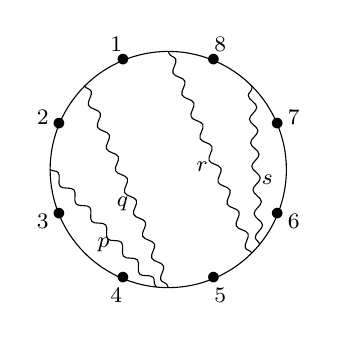
\begin{tikzpicture}[rotate=67.5,baseline=(current bounding box.east)]
	\begin{scope}
	\drawWLD{8}{1.5}
	\drawnumbers
	\drawlabeledprop{1}{0}{4}{0}{\footnotesize $q\ $}
	\drawlabeledprop{2}{0}{4}{-1}{\footnotesize $p$}
    \drawlabeledprop{5}{0}{8}{0}{\footnotesize $r\ \ $}
    \drawlabeledprop{5}{1}{7}{0}{\footnotesize $\ \ \ s$}

		\end{scope}
	\end{tikzpicture}\]

To construct $I_1$ we start at vertex 1, so we set $i=1$, $j = 1$, and $I_1 = \emptyset$. 
\begin{itemize}
\item $j = 1$: Since $\Prop(1) = \{q,r\}$ and $r$ is the clockwise-most of these propagators, we let $I_1 = \{1\}$ and remove propagator $r$ from the diagram. 
\item $j = 2$: $\Prop(2) = \{p,q\}$, with $q$ being the clockwise-most of these propagators. So $I_1 = \{1,2\}$ and propagator $q$ is removed.
\item $j = 3$: $\Prop(3) = \{p\}$, so now $I_1 = \{1,2,3\}$ and propagator $p$ is removed. The only remaining propagator in the diagram is $s$.
\item $j = 4$: Since $p$ and $q$ were removed in earlier steps, we now have $\Prop(4) = \emptyset$.
\item $j = 5$: $\Prop(5) = \{s\}$, and we have $I_1 = \{1,2,3,5\}$.
\end{itemize}
There are no propagators left in the diagram, so the algorithm terminates and we have ${I_1 = \{1,2,3,5\}}$, or $1235$ for short. So the propagators are ordered $r,q,p,s$ with respect to $I_1$, and $I_1$ viewed as a function is given by
\[I_1: \cP \longrightarrow [n] : \quad I_1(r) = 1,\quad I_1(q) = 2, \quad I_1(p) = 3, \quad I_1(s) = 5.\]
Applying the algorithm for all 8 starting vertices, we obtain the sets
\[1235, 2356, 3456, 4567, 5671, 6712, 7812, 8123.\]
The reader can easily verify that this sequence of $k$-sets satisfies the definition of a Grassmann necklace, and can (with significantly more work) also verify that this Grassmann necklace defines the positroid $M(W)$ associated to the Wilson loop diagram $W$ above.
\end{eg}



\begin{rmk}\label{rmk algorithm locally same}
The following observation about the local behavior of the algorithm will be very useful in many of the arguments below.

Suppose we are going through the algorithm to construct $I_i^W$ for some $i$, and we are currently at step $j$ of the loop.  Consider the diagram $W'$ formed by removing from $W$ all propagators that have already contributed to $I_i^W$. (This just replicates the behavior of the algorithm, which removes each propagator once it contibutes to $I_i^W$.)  Now suppose for some other diagram $V$ on the same vertex set we are constructing $I_m^V$ for some $m$, and we are at step $j$ of the loop, for the same $j$ as above.  Again obtain $V'$ from $V$ by removing all propagators assigned so far. \sanote{rewrote, do we like this?}\note{Sian: rewrote some more. We need to be a bit careful with ``contributes'' because $p$ is assigned, not contributed, by the algorithm: vertices are contributed, propagators contribute.}

With this setup, if we can find a vertex $\ell$ (with $\ell <_i i$ and $\ell <_m m$) such that the configuration of propagators ending in the interval $(j-1, \ldots, \ell+1)$ is identical in both $W'$ and $V'$, then the vertices contributed to $I_i^W$ and $I_m^V$ are the same from step $j$ to step $\ell$ (inclusive). See Figure~\ref{fig:locally identical} for an illustration of this.

\begin{figure}
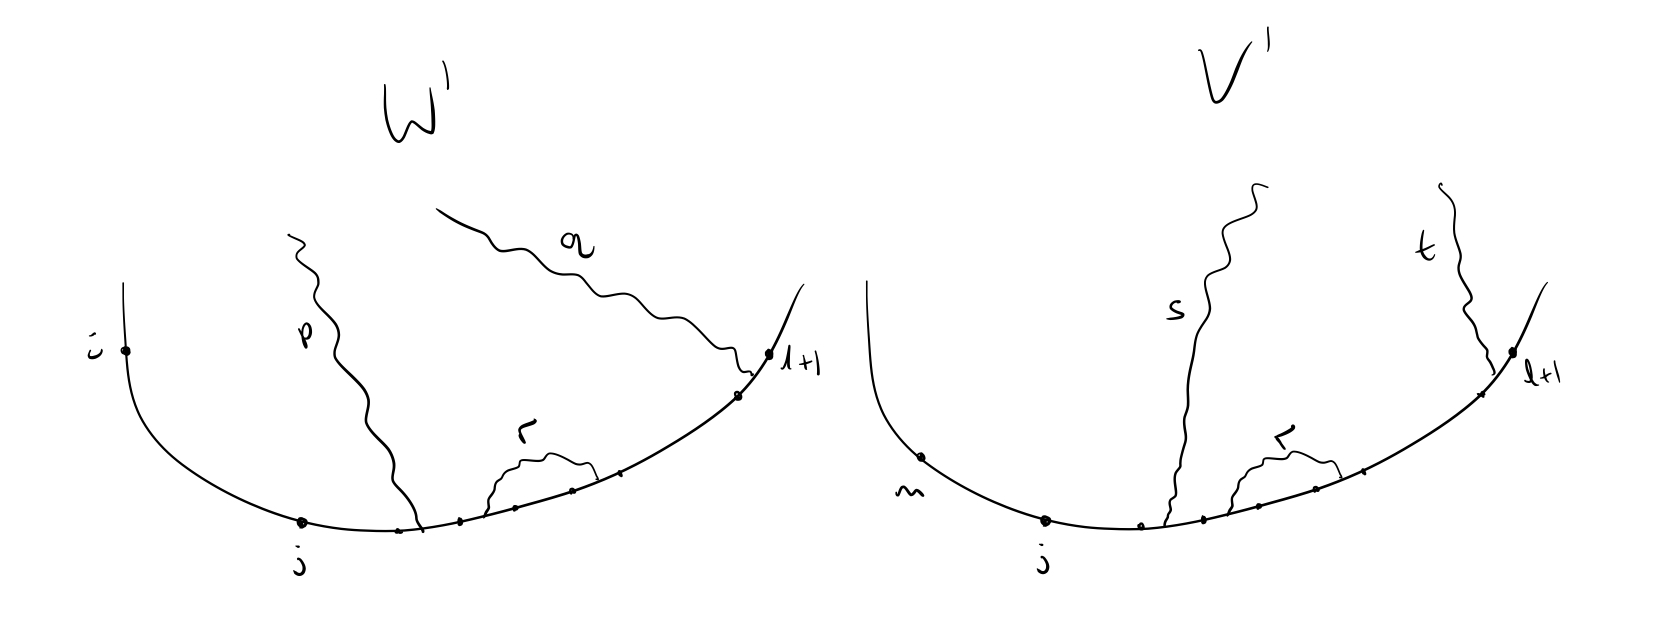
\includegraphics[scale=0.2]{locally_identical.jpg}
\caption{$W'$ and $V'$ are locally the same between $j$ and $l+1$, so we will have $I_i^W\cap [j,l] = I_m^V\cap[j,l]$ even though $p \neq s$ and $q \neq t$.}\label{fig:locally identical}
\end{figure}
\end{rmk}

With that in mind we are ready to begin proving properties of the algorithm. We first show that the algorithm can never reach the final vertex in a propagator's support without having already assigned that propagator; in particular, this guarantees that the construction of $I_i$ always terminates in fewer than $n$ steps.

\begin{lem}\label{lem no fourth vertex}
Let $W$ be an admissible Wilson loop diagram containing at least one propagator. For any $i \in [n]$ and for any $p \in \cP$, $I_i(p)$ is not maximal (with respect to $<_i$) amongst the vertices that support $p$.
\end{lem}
\begin{proof}
Suppose for contradiction that we have $i \in [n]$ and $p \in \cP$ such that $I_i(p)$ is $<_i$-maximal in $V(p)$. There are two possibilities, which are illustrated in Figure~\ref{fig:no fourth vertex}: either $p = (i-1,b)$ for some $b$ (so $i$ and $I_i(p) = i-1$ are the two ends of a single edge), or $p = (a,b)$ with $i\leq_i a <_i b$ and $I_i(p) = b+1$.

\begin{figure}
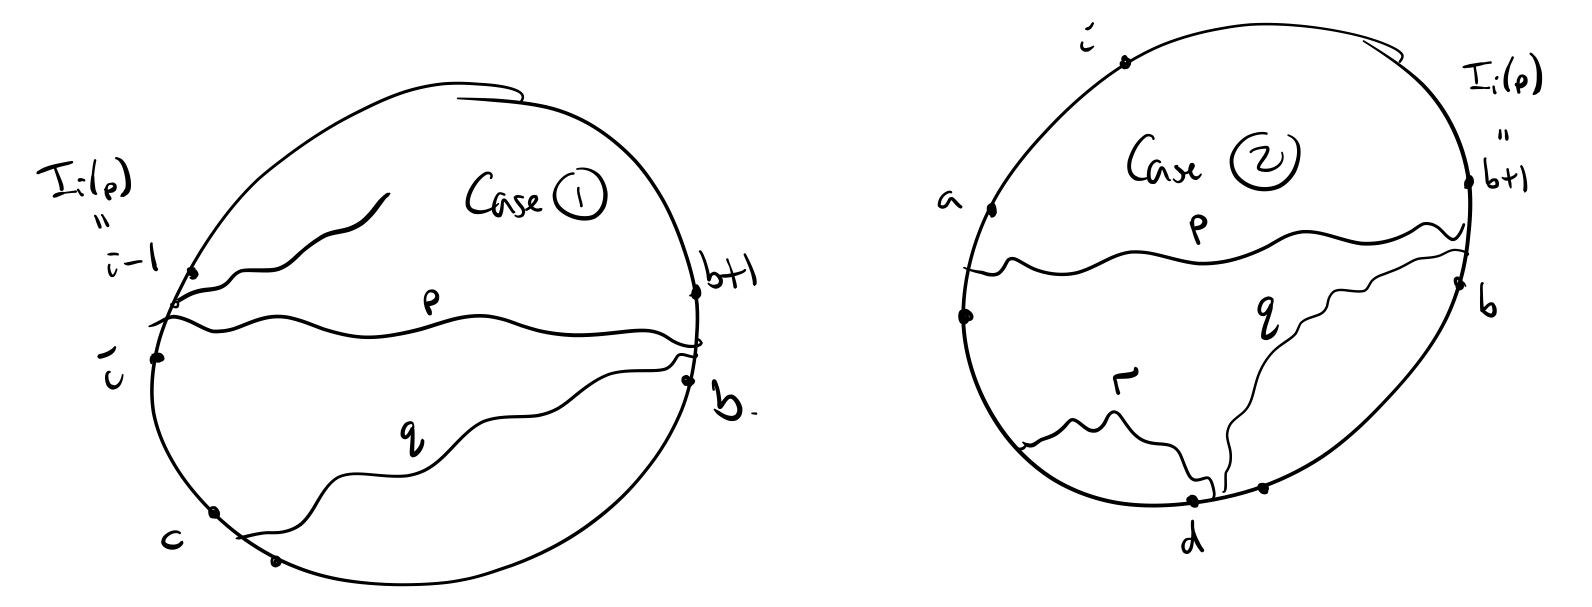
\includegraphics[width=15cm]{4th_vertex}
\caption{The two types of configuration in which a propagator could (in theory) contribute its $<_i$-maximal support vertex to $I_i$.}
\label{fig:no fourth vertex}
\end{figure}f

In the left hand case, observe that we must have another propagator $q = (c,b)$ with $c<_i b$ and $I_i(q) = b+1$, because otherwise $I_i$ would assign $p$ to $b+1$. Now $q$ also contributes the $<_i$-maximal vertex in its support to $I_i$ and is an instance of the right hand case listed above. Therefore it suffices to show that no admissible Wilson loop diagram admits the configuration illustrated in the right hand case of Figure~\ref{fig:no fourth vertex}.

So let $p = (a,b)$ with $a<_ib$ and $I_i(p) = b+1$, and choose $p$ such that $|[a+1,b]|$ is minimal amongst propagators of $W$ with this property.

Since $I_i(p) \neq b$, there must exist a propagator $q$ inside of $(p,<_i)$ with $I_i(q) = b$. The propagator $q$ cannot end on the edge $b-1$, as this would contradict the minimality of $p$, so we have $q = (d,b)$ with $a <_i d <_i b$, and $I_i(q) = b$. 

In order for $q$ to remain unassigned until vertex $b$, there must be another propagator $r$ with an end on edge $d$ and $I_i(r) = d+1$; the only way this can occur is if $r$ is outside of $(q,<_i)$ but inside $(p,<_i)$. But now $r$ contributes its fourth vertex to $I_i$, again contradicting the minimality of $p$.
\end{proof}

\begin{cor}\label{GN alg well defined}
If $W$ is an admissible Wilson loop diagram with $k$ propagators, then Algorithm~\ref{alg:put GN on WLD} assigns exactly $k$ distinct vertices to each $I_i$. \sanote{suddenly confused. Don't we need working about in going onely once around or somesuch?}\note{Sian: added the word ``distinct'' in the statement and a few words to the last line of the proof, does that help?}
\end{cor}
\begin{proof}
Fix $i \in [n]$. It follows from the proof of Lemma~\ref{lem no fourth vertex} that in applying Algorithm~\ref{alg:put GN on WLD} to construct the set $I_i$, the algorithm can never reach the fourth vertex of a propagator's support (ordered with respect to $<_i$) without having already assigned $p$. Therefore if the algorithm starts at vertex $i$, all propagators must have been eliminated by the time it gets to vertex $i-1$, ensuring that the algorithm is completed in less than one full circumnavigation of the diagram and that $I_i$ contains exactly $k$ distinct elements.
\end{proof}

We now reverse our perspective and ask: given a propagator $p$ and a vertex $i$ in the support of $p$, for which set of starting vertices does the algorithm assign $p$ to $i$? 






Specifically, for each $i$ in the support of $p$ we define the set
\[J_p^{W}(i) = \{m \in [n] \ | \ I^{W}_m(p) = i \},\]
the set of starting vertices $m$ such that $I_m^{W}$ assigns $p$ to $i$. 

The following lemma establishes that these sets behave in a simple and predictable manner, a fact which we will repeatedly use in subsequent proofs.




\begin{lem} \label{vertex cyclic int lem}
  
Let $W = (\cP,[n])$ be an admissible Wilson loop diagram, and $p = (i,j) \in \cP$.  Then $J_p^{W}(i)$, $J_p^{W}(i+1)$, $J_p^{W}(j)$, and $J_p^{W}(j+1)$ are each non-empty cyclic intervals which partition $[n]$ and occur in the given cyclic order.
\end{lem}
\note{Right at the end when we put the tikz figures in, someone needs to go through this proof and replace ``leftmost two cases'' with ``Case 1 and 2'' etc, because the tikz picture is arranged differently}

\begin{proof}
We will prove the result by induction on the number of propagators.  If $W$ has one propagator then the result is immediate.  Now suppose $W$ has more than one propagator.  Since non-supporting vertices have no effect on Algorithm~\ref{alg:put GN on WLD}, it suffices to prove the result for $W$  (possibly weakly admissible) with $F(\emptyset) = \emptyset$.  Then by Lemma~\ref{lem sian}, $W$ has at least one of the four situations illustrated in Figure~\ref{fig 3 cases}.

\begin{figure}
    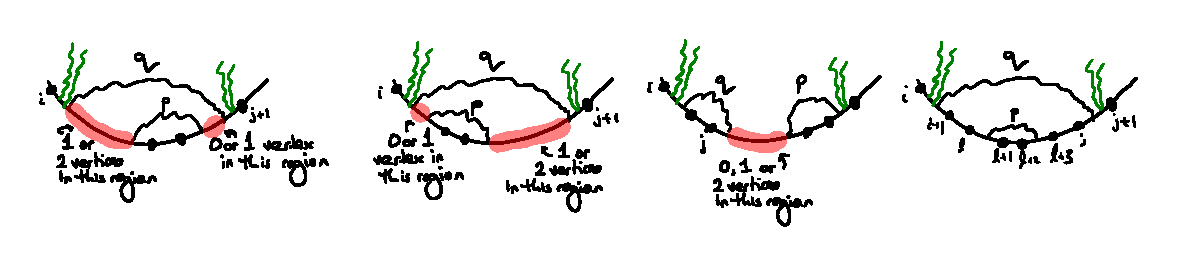
\includegraphics[scale=0.8]{3cases}
    \caption{Four cases for admissible WLDs with no non-supporting vertices. The green half-propagators illustrate where propagators may occur, but are not required to exist; no other regions illustrated may support additional propagators.}\label{fig 3 cases}
  \end{figure}


In each of the four cases, when we remove the propagator labelled $p$ we obtain a diagram which satisfies the statement of the theorem by the induction hypothesis, and contains a propagator ${q = (i,j)}$ with no other propagators inside it (with respect to the $<_i$ orientation). Note that this region may or may not contain non-supporting vertices, which we will call $l, l+1, \ldots$ as necessary. Let $V$ be the diagram obtained by removing the propagator $p$ from $W$ (Figure \ref{fig V diagram}). $V$ is guaranteed to be an admissible diagram, since it was formed by removing a propagator from a diagram that was at least weakly admissible.


\begin{figure}
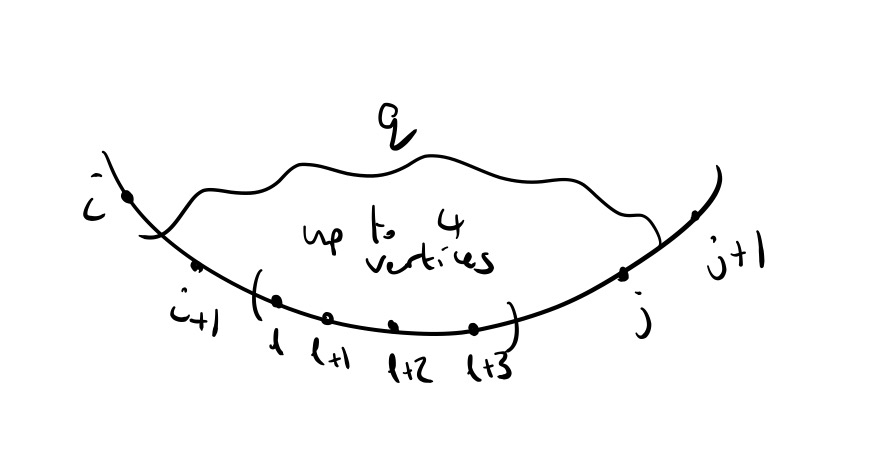
\includegraphics[width=10cm]{V_diagram}
\caption{Diagram $V$ is $W$ with $p$ removed; there are no propagators inside $q = (i,j)$, though there may be up to 4 non-supporting vertices labelled $l, l+1, \ldots$.}
\label{fig V diagram}
\end{figure}


Consider the fourth case of Figure~\ref{fig 3 cases} first, as it is the easiest.  In this case, the vertices ${\{l,l+1,l+2,l+3\}}$ which support $p$ in $W$ are non-supporting in $V$, so for every propagator $r$ in $V$ (including $q$) we have $J_r^{V} = J_r^{W}$; these are non-empty cyclic intervals in the correct order by the induction hypothesis.  Additionally, it is clear from Figure~\ref{fig 3 cases} that $J_p^{W}(l+a) = \{l+a\}$ for $a\in\{1,2,3\}$ and $J_p^{W}(l) = [n] \backslash \{l+1, l+2, l+3\}$. The result therefore holds in this case.


Now we proceed to consider the first three cases of Figure~\ref{fig 3 cases}.
We first describe $J_q^{V}(*)$, which can be handled identically for all three cases.

In $V$ there are no propagators inside $q$ by construction, so we see from Figure \ref{fig V diagram} that
\[l, l+1, \ldots ,j \in J^{V}_q(j) \text{ (if $l$ exists) and }  j+1 \in J^{V}_q(j+1).\]
Note that $j+2 \not\in J^{V}_q(j+1)$ by Lemma~\ref{lem no fourth vertex}, so  $J^{V}_q(j+1) = \{j+1\}$ and by the induction hypothesis we must have $j+2 \in J^{V}_q(i)$. Thus there exist vertices $d,e \in [j+2,i+1]$ with $d <e$, such that
\ba J^{V}_q(i) = [j+2,d-1], \quad J^{V}_q(i+1) = [d,e-1], \quad J^{V}_q(j) = [e,j], \quad J^{V}_q(j+1) = \{j+1\}, \label{deeqs}\ea
and all intervals are non-empty.




We now consider what happens as we move from $V$ to each of the three remaining cases for $W$. We need to consider both $J^{W}_p$ and $J^{W}_r$ for $r \neq p$, since the addition of $p$ can have a knock-on effect on later steps in the algorithm.

%%%%%%%%%

\textbf{Left two cases}: These cases behave essentially identically (except when $j$ or $j+1$ are not in the support of $p$, which can occur in the second case only; see below) so we handle the majority of the proof for these two cases simultaneously. Write $p=(m,m+2)$ where $m\in \{i, i+1, l\}$. Let $1\leq a\leq 3$ be the number of non-supporting vertices inside $q$ in $V$ (note that there is at least 1); so these vertices are $l, \ldots, l+a-1$.  Note that these non-supporting vertices are all in the support of $p$. 

We first calculate $I^{W}_w$ for a starting vertex ${w \in [n]\backslash \{l, l+1, \ldots,j,j+1\}}$. Note that $p$ has no effect on other propagators for starting vertices in this range, so if $r \neq p$, then $I_w^W(r) = I_w^V(r)$. Meanwhile, the value of $I^{W}_w(p)$ depends on which step in the algorithm the propagator $q$ is assigned to a vertex, i.e. on the value of $I^{V}_w(q)$. Thus, if $w\in J_q^{V}(i)$ then 
    \[
    I_w^{W}(r) =  \begin{cases}
        \max\{i+1, m\} & \text{if } r=p \\
        I_{w}^{V}(r) & \text{if } r\neq p
      \end{cases} 
    \]
    while if $w\in J_q^{V}(i+1)$ or $w\in J_q^{V}(j)$ then
    \[
    I_w^{W}(r) =  \begin{cases}
        l & \text{if } r=p \\
        I_{w}^{V}(r) & \text{if } r\neq p
      \end{cases} 
      \]
We also need to understand $I^{W}_w$ for $w \in \{l,l+1,\ldots,j,j+1\}$. For the majority 
%$w \in [l, l+a-1]$} 
%I left this as a comment so we can add it in if necessary, but I don't think we need this level of precision in this sentence: we're just signposting what we're going to do in detail shortly.
of these vertices, we use the following observation: if $p$ is the first propagator to be assigned a value by $I_w^{W}$, then the remainder of $I_w^{W}$ proceeds identically to the assignments of $I^{V}_{w+1}$ (recall Remark~\ref{rmk algorithm locally same}).  Thus we have for any $0\leq b <a$
    \[
    I_{l+b}^{W}(r) = \begin{cases}
      l+b & \text{if } r=p\\
      I_{l+b+1}^{V}(r) & \text{if } r\neq p
    \end{cases}
    \]
Similarly, if $j$ is in the support of $p$, then we have
     \[
       I_j^{W}(r) = \begin{cases}
         j & \text{if $r=p$ and $j$ is in the support of $p$}\\
         I_{j+1}^{V}(r) & \text{if $r\neq p$ and $j$ is in the support of $p$}\\
       \end{cases}
       \]
If $j$ is not in the support of $p$, then we must be in the second case of Figure~\ref{fig 3 cases} with two vertices in the right hand region.  In this case, if we start the algorithm at $j$ we need to know whether there will be any unassigned propagators other than $p$ when we reach vertex $i$, so as to know what $p$ contributes.

Consider the Wilson loop diagram $X$ formed from $V$ by replacing the propagator $q = (i,j)$ with $q = (i, j-1)$; \note{Added a note about $V$ being admissible when we defined it, so we can use $X$ admissible here without comment} $X$ is still admissible since we have not decreased the support of any set of propagators. 
% From the diagram we can see that $J_{j}^{V}(r) = J_{j}^{X}(r)$ for all $r\neq p$ (and in particular for $r=q$) and $J_{j}^{X}(r) = J_{j+1}^{X}(r)$ for $r\neq q,p$.  
It follows from the position of $q$ in $X$ that $I_j^X(q) = j$, and from Lemma~\ref{lem no fourth vertex} that $I_{j+1}^X(q) \neq j$. By the induction hypothesis, we must therefore have $I_{j+1}^X(q) = i$; in particular, this means that if we start at $j+1$ and assign propagators to vertices according to the algorithm, when we reach vertex $i$ in $X$ all propagators other than $q$ must have been assigned.

Therefore if we start at $j$ in $W$, we first assign $q$ to $j$ then proceed to assign as in $X$ starting at $j+1$, and hence when we get to $i$ the only remaining unassigned propagator is $p$. We obtain
       \[
       I_j^{W}(r) = \begin{cases}

       m & \text{if $r =p$ and $j$ is not in the support of $p$} \\
       I_{j}^{V}(r) & \text{if $r\neq p$ and $j$ is not in the support of $p$}\end{cases}
       \] 
This completes the analysis of $I_j^W$. Finally, we consider what happens when we start the algorithm at vertex $j+1$. If $j+1$ is in the support of $p$ then we can argue as above to get
\[
       I_{j+1}^{W}(r)  = \begin{cases}
         j+1 & \text{if $r=p$ and $j+1$ is in the support of $p$}\\
         I_{j+2}^{V}(r) & \text{if $r\neq p$ and $j+1$ is in the support of $p$}.
       \end{cases}
       \]
Now suppose $j+1$ is not in the support of $p$. If we start at $j+1$ we need to know whether there are any unassigned propagators supported on edge $i$ when we reach vertex $i$. We already know that $J_q^{V}(j+1) = \{j+1\}$; in particular this means that $q$ contributes $i$ in $I_{j+2}^{V}$, by the induction hypothesis applied to $V$. However the construction of $I^{V}_{j+1}$ first assigns $q$ to $j+1$ and then proceeds identically to $I^{V}_{j+2}$.  In particular if $i$ was assigned in $I^{V}_{j+1}$, then it would not be available to assign to $q$ in $I^{V}_{j+2}$ as all other propagators supported at $i$ in $V$ come before $q$. 

Therefore $p$ is the only potentially unassigned propagator on edge $i$ when we reach vertex $i$ in the algorithm for $I_{j+1}^W$, and
    \[
    I_{j+1}^{W}(r)  = \begin{cases}
      m & \text{if  $r=p$ and $j+1$ is not in the support of $p$}\\
      I_{j+1}^{V}(r) & \text{if  $r\neq p$ and $j+1$ is not in the support of $p$}
    \end{cases}
    \]
We can now describe the intervals $J^{W}_r(*)$ for the first two cases of Figure~\ref{fig 3 cases}. For $r \neq p$ the intervals are clearly still cyclic and appear in the correct order, and we can assemble the intervals for the $J_p^{W}(*)$ as follows. Recall that $p = (m,m+2)$, $1 \leq a \leq 3$ is the number of non-supporting vertices inside $q$ in $V$, and these non-supporting vertices are denoted $\{l,l+1, \dots\}$. 
    \begin{itemize}
      \item 
    If $m=l$ then either $a=2$ (so $l+1=m+1$, $j=m+2$, and $j+1=m+3$) or $a=3$ (so $l+1=m+1$, $l+2=m+2$, $j=m+3$, and $j+1$ is not in the support of $p$), and in both cases
    \begin{gather*}
    J^{W}_p(m) = [m+4, m], \qquad  J^{W}_p(m+1) = \{m+1\}, \\ J^{W}_p(m+2) = \{m+2\}, \qquad  J^{W}_p(m+3) = \{m+3\},
    \end{gather*}
    which are nonempty and otherwise as required.
  \item
        If $m=i+1$ then checking each of the three different possibilities for $a$ we likewise get
    \begin{gather*}
    J^{W}_p(m) = [m+4, d-1], \qquad  J^{W}_p(m+1) = [d, m+1], \\  J^{W}_p(m+2) = \{m+2\}, \qquad  J^{W}_p(m+3) = \{m+3\},
    \end{gather*}
    which are nonempty and otherwise as required. Recall that $d$ was defined in equation \eqref{deeqs}.
  \item If $m=i$ then $a=1$ or $a=2$, in the former case $l=m+2$, $j=m+3$ and $j+1$ is not in the support of $p$ so
    \begin{gather*}
    J^{W}_p(m) = \{m+4\}, \qquad  J^{W}_p(m+1) = [m+5, d-1], \\  J^{W}_p(m+2) = [d, m+2], \qquad  J^{W}_p(m+3) = \{m+3\},
    \end{gather*}
    while in the latter $l=m+2$, $l+1=m+3$, and $j$ and $j+1$ are not in the support of $p$ so
    \begin{gather*}
    J^{W}_p(m) = [m+4, j+1], \qquad  J^{W}_p(m+1) = [j+2, d-1], \\  J^{W}_p(m+2) = [d, m+2], \qquad  J^{W}_p(m+3) = \{m+3\},
    \end{gather*}
    which are again as required.
    \end{itemize}

\textbf{Third case}: In this case there are no non-supporting vertices $l, l+1, \ldots$ inside $q$.  Again write $p=(m, m+2)$ where $m\in \{j, j+1, j+2\}$. We proceed as in the previous cases, by computing $I^{W}_w$ for vertices $w$ in roughly increasing order of difficulty.

For $w \in [n]\backslash\{j+1,m,m+1,m+2,m+3\}$: if $w\in J_q^{V}(i)$ or $w\in J_q^{V}(i+1)$ then
    \[
    I_w^{W}(r) =  \begin{cases}
        m & \text{if } r=p \\
        I_{w}^{V}(r) & \text{if } r\neq p
      \end{cases} 
    \]
    while if $w\in J_q^{V}(j)$ then
    \[
    I_w^{W}(r) =  \begin{cases}
        \max\{m, j+1\} & \text{if } r=p \\
        I_{w}^{V}(r) & \text{if } r\neq p
      \end{cases} 
    \]

Finally, for $j+1$ and the vertices in the support of $p$, we have

\begin{align*}
  I_{j+1}^{W}(r) &= \begin{cases}
    j+1 & \text{if } r=q\\
    j+2 & \text{if } r=p\\
    I_{j+3}^{V}(r) & \text{if } r\neq p,q
  \end{cases}\\
  I_m^{W}(r) &= \begin{cases}
    m & \text{if $r=p$ and $q$ not supported on $m$}\\
    m+1 & \text{if $r=p$ and $q$ supported on $m$}\\
    I_{m}^{V}(r) & \text{if } r\neq p
  \end{cases}\\
  I_{m+1}^{W}(r) & = \begin{cases}
    m+1 & \text{if $r=p$ and $q$ not supported on $m+1$} \\
    m+2 & \text{if $r=p$ and $q$ supported on $m+1$} \\
    I_{m+1}^{V}(r) & \text{if } r\neq p,q
  \end{cases}\\
  I_{m+2}^{W}(r) & = \begin{cases}
    m+2 & \text{if } r=p \\
    I_{m+3}^{V}(r) & \text{if } r\neq p
  \end{cases}\\
  I_{m+3}^{W}(r) & = \begin{cases}
    m+3 & \text{if } r=p \\
    I_{m+4}^{V}(r) & \text{if } r\neq p
  \end{cases}
\end{align*}
Note that $I_{m+2}^{V}(r) = I_{m+3}^{V}(r)$ for all propagators $r$ in $V$, and that if $j+1\not\in\{m, m+1, m+2, m+3\}$ then $j+2$ and $j+3$ are non-supporting vertices in $V$, so in that case $I_{j+2}^{V}(r) = I_{j+3}^{V}(r) = I_{j+4}^{V}(r)$ for $r$ in $V$. 

Therefore, once again we can see that the $J_r^{W}(*)$ are cyclic for all $r\neq p$ in $W$.  Assembling the intervals for $p$ we have:
\begin{itemize}
\item If $m=j$ then
\begin{gather*}J_p^{W}(m) = [m+4,e-1], \qquad  J_p^{W}(m+1) = [e,m], \\  J_p^{W}(m+2) = [m+1,m+2], \qquad  J_p^{W}(m+3) = \{m+3\},\end{gather*}
Recall that $e$ was defined in equation \eqref{deeqs}.
\item If $m=j+1$ then
\begin{gather*}J_p^{W}(m) = [m+4,m-1], \qquad J_p^{W}(m+1) = [m,m+1], \\  J_p^{W}(m+2) = \{m+2\}, \qquad  J_p^{W}(m+3) = \{m+3\},\end{gather*}
\item If $m=j+2$ then
\begin{gather*}J_p^{W}(m) = [m+4,m], \qquad  J_p^{W}(m+1) = \{m+1\}, \\  J_p^{W}(m+2) = \{m+2\}, \qquad  J_p^{W}(m+3) = \{m+3\}.\end{gather*}
\end{itemize}
The result now follows by induction.
\end{proof}



We are now ready to prove that Algorithm~\ref{alg:put GN on WLD} does in fact give the Grassmann necklace of the positroid associated to $W$.

\begin{thm}\label{res:alg gives GN}
The sequence of $k$-subsets $(I_1,\dots,I_n)$ obtained by applying Algorithm~\ref{alg:put GN on WLD} to all vertices of an admissible diagram $W$ is exactly the Grassmann necklace of $M(W)$.
\end{thm}
\begin{proof}
For each $i \in [n]$, let $I_i$ be the set of vertices assigned to the propagators of $W$ by Algorithm~\ref{alg:put GN on WLD} with starting vertex $i$. By Lemma~\ref{GN alg well defined}, we know that $|I_i| = k$ for each $i \in [n]$. We first prove that $I_{i+1} \supseteq I_i \backslash \{i\}$ for all $i \in [n]$; this is equivalent to the definition of Grassmann necklace given in Definition~\ref{def:grassmann necklace}.

Suppose for a contradiction that there exists an admissible diagram for which there exists an $i$ with $m\in I_i\setminus \{i\}$ and $m \not\in I_{i+1}$.  Fix $n$.  Let the triple $(W, i, m)$ be such a counterexample on $n$ vertices which is minimal with respect to the number of propagators. %, and among all those counterexamples on $n$ vertices with the same number of propagators, let $(W,i,k)$ be minimal with respect to the distance from $i$ to $k$ in the $\leq _i$ order.

If $i \not\in I_i$, then there are no propagators supported on $i$ at all.  In this case it is clear that applying Algorithm~\ref{alg:put GN on WLD} at vertex $i$ and vertex $i+1$ produces exactly the same result, i.e. $I_{i+1} = I_i$, and so $(W, i, m)$ is not a counterexample at all.

Now suppose that $i \in I_i$.  Let $p$ be the propagator which contributes $i$ to $I_i$, that is $I^W_i(p) = i$; thus one end of $p$ must lie on either edge $i-1$ or edge $i$.  In both cases let $b$ denote the edge supporting the other end of $p$, i.e. $p = (i, b)$ or $p = (i-1, b)$.


\textbf{Case I}:  Suppose $p$ has one end on edge $i-1$.  If $p$ is not supported on $i+1$, then in building $I_{i+1}$ we will assign the same propagators as in the construction of $I_i$ from vertices $i+1$ up to $b-1$, that is $I_{i+1} \cap [i+1,b-1] = I_{i} \cap [i+1,b-1]$.  (If $p$ is supported on $i+1$, then $b= i+1$ and the interval $[i+1,b-1]$ is empty.) Furthermore, by Lemma~\ref{vertex cyclic int lem} it must happen that $p$ contributes vertex $b$ to $I_{i+1}$, as otherwise $b$ would never be contributed by $p$. Consequently, in building $I_{i+1}$, when the algorithm reaches vertex $b$ there cannot be any remaining unassigned propagators that are supported on $b$ and counterclockwise of $p$.  This is also true in when the algorithm constructing $I_i$ reaches $b$, since the same propagators have been assigned beforehand.  Finally, we also note that $m\geq_i b+1$.

Let $W' = (\cP_{out}(p,<_i), [n])$, i.e. the diagram obtained from $W$ by removing both $p$ and all propagators inside of $p$.

By the above observations, if we commence Algorithm~\ref{alg:put GN on WLD} in $W'$ from vertex $b$, then we are in the same situation with respect to unassigned propagators as if we began at $i$ in $W$ and proceeded to $b$ following the algorithm (recall that $I^W_i(p) =i$). The propagators contributing to $I_{i}^W$ before the vertex $b$ are exactly the ones removed in the construction of $W'$.  Similarly, starting at $i+1$ in $W$ and moving to $b+1$ leaves us in the same situation with respect to unassigned propagators as beginning at $b+1$ in $W'$ would.  This gives the equations
\begin{align*}
  I_i^{W} \cap [b,i-1] & = I_b^{W'} \\
  I_{i+1}^{W} \cap [b+1,i-1] & = I_{b+1}^{W'}
\end{align*} 
where the diagram is indicated in the superscript.
Thus we have $m\in I_b^{W'}\setminus\{b\}$ and $m\not\in I_{b+1}^{W'}$, contradicting the minimality of $(W, i, m)$.

\textbf{Case II}: Suppose $p$ has one end on edge $i$.  Note that by assumption we have $I_i(p) = i$; this means that $p$ must be the counterclockwise-most propagator lying on edge $i$, and hence we must have $I_{i+1}(p) = i+1$ as well.  Observe also that $m\geq_i i+2$ since $i+1\in I_{i+1}$.

Let $W'$ be the diagram obtained from $W$ by removing only the propagator $p$.  Then we have
\begin{align*}
  I_i^{W} \backslash \{i\} & = I_{i+1}^{W'} \\
  I_{i+1}^{W} \backslash \{i+1\} & = I_{i+2}^{W'}
\end{align*}
since in both cases the algorithm in $W'$ proceeds identically to that in $W$ after assigning $p$. Since $m \neq i+1$, we have $m\in I_{i+1}^{W'}\setminus\{i+1\}$ but $m\not\in I_{i+2}^{W'}$, contradicting the minimiality of $(W, i, m)$.


\medskip  \sanote{Suggested breakpoint of theorem}

We have shown that $(I_1,\dots,I_n)$ is a Grassmann necklace; it remains to check that this Grassmann necklace corresponds to the positroid $M(W)$.  Recall from the discussion following Definition~\ref{def:grassmann necklace}, and equation \eqref{basesofmatroids} in particular, that it suffices to show: 
\begin{itemize}
\item For each $i \in [n]$, $I_i$ is a basis for $M(W)$.
\item If $J$ is lexicographically smaller than $I_i$ with respect to $<_i$ (for any $i \in [n]$) then $J$ is not a basis for $M(W)$. 
\end{itemize}
The first point follows immediately: since the algorithm is pairing each $j \in I_i$ with a unique propagator supported on that vertex, $I_i$ is a basis for $M(W)$ by Corollary~\ref{lem basis as perm}.

Now suppose we have a $k$-set $J$ such that $J$ is a basis for $M(W)$ and yet is lexicographically less than $I_i$ with respect to $<_i$.  By Corollary~\ref{lem basis as perm} there is a set bijection between $J$ and the propagators of $W$ such that for each $j \in J$, the propagator associated to $j$ is supported on vertex $j$.  Choose one such bijection.  For each propagator $p$ of $W$, write $J(p)$ for the vertex $j$ associated to $p$ according to this bijection.

Since $J$ is lexicographically smaller than $I_i$, the $<_i$-smallest element of the symmetric difference of $J$ and $I_i$ is some $j_0\in J$, $j_0 \not\in I_i$. Let $p_1$ be the propagator such that $J(p_1)=j_0$.  Since $j_0\not\in I_i$ but $p_1$ is supported at $j_0$, then $p_1$ must have been assigned to an earlier vertex by $I_i$, i.e. we have $I_i(p_1) <_i j_0$.  Let $j_1 = I_i(p_1)$.

However, $j_0$ is the $<_i$-smallest element in the symmetric difference of $J$ and $I_i$, so we must have $j_1 \in J$ as well; in particular, there is some propagator $p_2$ such that $J(p_2)=I_i(p_1)$.  Let $j_2 = I_i(p_2)$ and note that $j_2 \neq J(p_2)$ (since $I_i(p_1)=J(p_2)$), so either $I_i(p_2) \not\in J$ or there is a propagator $p_3$ such that $J(p_3) = I_i(p_2)$. Continue this process for as many steps as possible (i.e. for as long as $I_i(p_*) \in J$); this produces a list of vertices $j_r$ and propagators $p_r$ such that 
\[J(p_r) = I_i(p_{r-1}) = j_{r-1}.\]

We claim that there is no repetition of propagators or vertices in this list; this will show that the process must eventually terminate. The claim is proved by induction.  The definition of $j_0$ gives that $j_0$ and $j_1$ are distinct and that $p_1$ and $p_2$ are distinct.  Now, suppose we have $p_r$ and $j_r$ with $I_i(p_r)=j_r$, with $j_r$ distinct from all previous $j_*$ and with $j_r\in J$.  Then there must exist a propagator $p_{r+1}$ with $J(p_{r+1}) = j_r$.  Since $J: \cP \longrightarrow [n]$ is injective and $j_r$ is not equal to any of the previous vertices $j_0, \dots, j_{r-1}$ by assumption, $p_{r+1}$ must be distinct from the previous propagators $p_1,\dots,p_r$.  Following the pattern, define $j_{r+1} = I_i(p_{r+1})$. Since $I_i: \cP \longrightarrow [n]$ is also injective and $p_{r+1}$ is distinct from the earlier $p_*$, it follows that $j_{r+1}$ is distinct from the other $j_s$ for $1\leq s\leq r$.  Finally, we have $j_{r+1}\neq j_0$ since $j_0\not\in I_i$ but $j_{r+1}\in I_i$.  This proves the claim.

Therefore the list must end, and the only way it can end is with some $p_r$ such that $j_r = I_i(p_r)\not\in J$. In particular, this implies that $j_r >_i j_0$.  

Next we will prove that $j_r <_i j_0$ for all $r > 0$; this gives a contradiction to the existence of $J$ and completes the proof of the theorem.  This proof will also be by induction; however, for the induction to go through nicely we will need to prove the following slightly stronger statement:
for all $r>0$ in the list
\begin{itemize}
\item $j_r <_i j_0$ and
\item either
  \begin{itemize}
  \item $I_i(p_r) <_i J(p_r)$, or
  \item there exists an $\ell<r$ such that $I_i(p_\ell) <_i J(p_\ell)$, those two vertices support distinct ends of $p_\ell$, and $p_r$ is inside $p_l$ when $p_l$ is directed from $I_i(p_\ell)$ to $J(p_\ell)$.\note{Should I replace this with ``$p_r$ is inside $(p_l,<_i)$''? It matches previous notation but maybe is less clear?}
  \end{itemize}
\end{itemize}

We observed above that $j_1 <_i j_0$ and $I_i(p_1) <_i J(p_1)$ so we have the base case for the induction.  Now fix $r > 1$ and suppose that the inductive hypothesis holds for all indices less than $r$ and that $p_r$ exists.

By definition $J(p_r) = I_i(p_{r-1}) = j_{r-1}$, so $p_{r-1}$ and $p_{r}$ are both supported at vertex $j_{r-1}$. 



Since $I_i$ always chooses the earliest unassigned propagator supported at a vertex, we have two possibilities (which are not mutually exclusive): either $p_{r-1}$ appears before $p_r$ in the neighbourhood of $j_{r-1}$, or $p_r$ was assigned earlier than $p_{r-1}$ by the algorithm for $I_i$. (Note that the ordering $p_1,p_2,\dots,p_r$ need not match the order in which Algorithm~\ref{alg:put GN on WLD} assigns propagators to vertices.)

In the latter case we are done, since $p_r$ being assigned earlier than $p_{r-1}$ by $I_i$ means exactly that $I_i(p_r) <_i I_i(p_{r-1})$. Recalling that $I_i(p_{r-1}) = J(p_r) = j_{r-1}$, this implies that $I_i(p_r) <_i J(p_r)$ and $j_r = I_i(p_r) <_i j_{r-1} <_i j_0$, as required. 

Now assume that $p_{r-1}$ appears before $p_r$ in the neighbourhood of $j_{r-1}$, and that $I_i$ assigns $p_{r-1}$ before $p_r$.



\hlfix{If $I_i(p_{r-1}) <_i J(p_{r-1})$ and these are vertices supported by distinct ends of $p_{r-1}$}{Sian was unsure about this sentence, and added the blue text below which may or may not be necessary}, then by our assumption that $p_{r-1}$ appears before $p_r$ in the neighbourhood of $j_{r-1}$ it follows that $p_r$ must lie inside $p_{r-1}$ when directed from $I_i(p_{r-1})$ to $J(p_{r-1})$.  Therefore 
\[j_r = I_i(p_r) \leq_i J(p_{r-1}) + 1.\]
If $r > 2$ then this gives $j_r \leq_i I_i(p_{r-2}) + 1 \leq_i j_0$, but we know that $j_0\not\in I_i$ so in fact we have a strict inequality $j_r<_i j_0$.  If $r=2$ then the inequality reads $j_2 \leq_i J(p_1) + 1 = j_0 + 1$, so either $j_2 <_i j_0$ or we have the configuration
\[
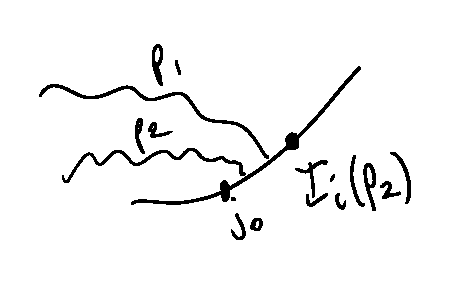
\includegraphics{impossible_config}
\]
However, this is impossible because now $p_2$ is supported at $j_0$ but not assigned by $I_i$ until after $j_0$, even though $j_0\not\in I_i$. Thus we always have $j_r <_i j_0$ and the inductive step is complete in this case (with $p_{r-1}$ playing the role of $p_l$ here).

\textcolor{blue}{
On the other hand, if $I_i(p_{r-1}) <_i J(p_{r-1})$ and these vertices are on the same end of $p_{r-1}$, then we must have 
\[
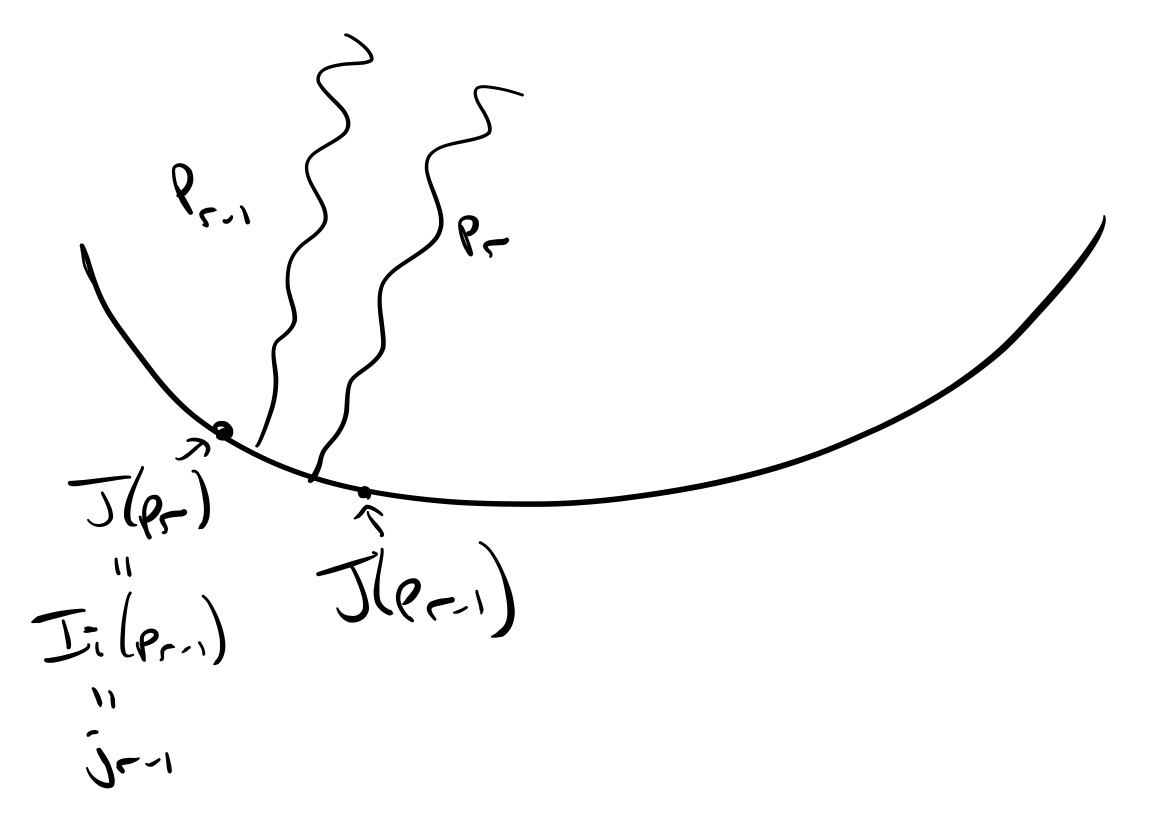
\includegraphics[width=10cm]{extra_config}
\]
If $r = 2$, then $J(p_{r-1}) = j_0$ and our assumption that $p_{r-1}$ is assigned before $p_r$ means that $I_i$ assigns $p_2$ to $j_0$, which is again a contradiction. If $r>2$ then $J(p_{r-1}) = I_i(p_{r-2})$ implies we have another propagator $p_{r-2}$ on this same edge, which must lie between $p_{r-1}$ and $p_r$ to ensure that $I_i$ assigns everything in the correct order. Now $J(p_{r-2})$ must support the other end of $p_{r-2}$, and we can apply the same argument as above with $p_{r-2}$ instead of $p_{r-1}$.}

The only remaining possibility is that $I_i(p_{r-1})\not<_i J(p_{r-1})$, so now assume this. We continue to assume that $p_{r-1}$ appears before $p_r$ in the neighbourhood of $j_{r-1}$ and that $I_i$ assigns $p_{r-1}$ before $p_r$.

By the induction hypothesis,  $I_i(p_{r-1})\not<_i J(p_{r-1})$ implies that there exists an $\ell < r-1$ such that $p_{r-1}$ lies inside $p_{\ell}$ when directed from $I_i(p_\ell)$ to $J(p_\ell)$. Since $p_{r-1}$ and $p_r$ are both supported on vertex $j_{r-1}$, either $p_r$ is also inside $p_l$ (in which case we apply the arguments above with $l$ instead of $r-1$) or $p_l$ lies between $p_{r-1}$ and $p_r$ in the neighbourhood of $j_{r-1}$.

Since $I_i(p_{r-1}) = j_{r-1}$ and $p_{r-1}$ is inside $p_l$, the fact that no propagator can contribute its 4th vertex to $I_i$ (Lemma~\ref{lem no fourth vertex}) means that we have the following configuration:
\[
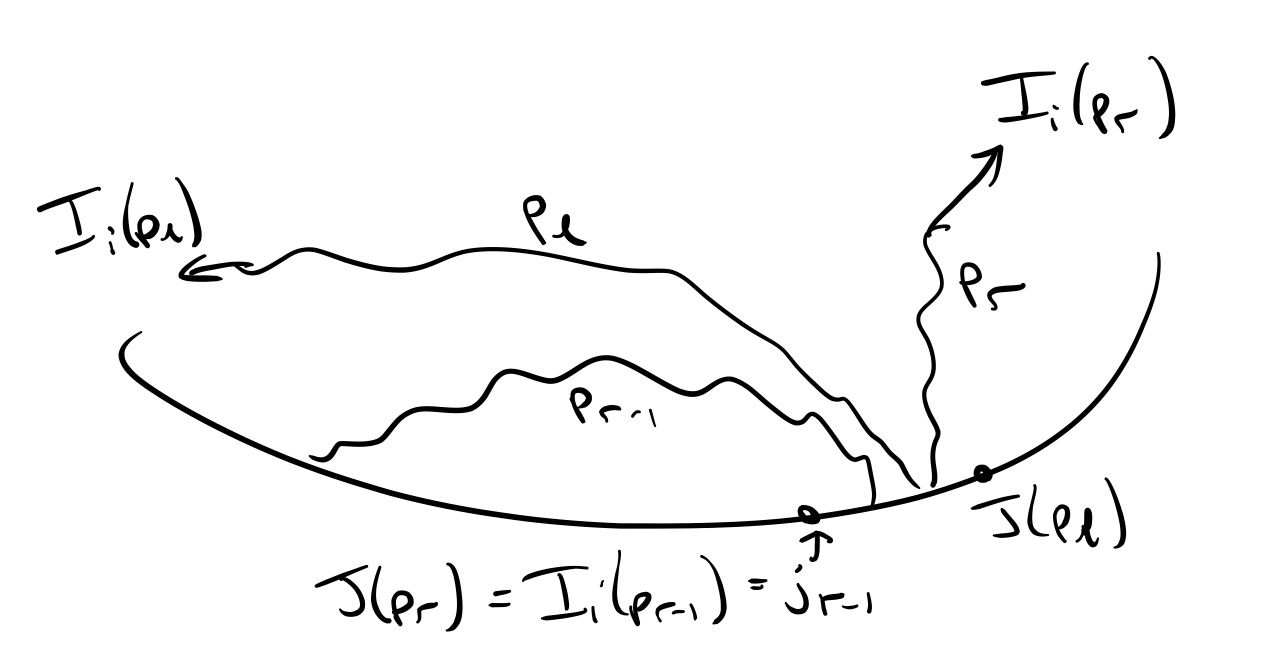
\includegraphics[width=10cm]{new_induction_conf}
\]
If $l=1$ then $J(p_l) = j_0$, and $p_r$ is supported on $j_0$ but assigned by $I_i$ later than $j_0$, which is a contradiction. If $l>1$ then $J(p_l) = I_i(p_{l-1})$, and propagator $p_{l-1}$ must appear before $p_r$ in the neighbourhood of $j_{r-1}$ to ensure that $I_i$ assigns $p_{l-1}$ correctly. But now $J(p_{l-1})$ must be on the other end of $p_{l-1}$, since the vertices on this end are $J(p_r)$ and $J(p_l)$ and we know that $l-1 < l < r$. Finally, we must have $I_i(p_{l-1}) <_i J(p_{l-1})$ so that $I_i$ does not assign $p_{l-1}$ to its fourth vertex. Now $p_r$ lies inside $p_{l-1}$ and we argue as above.


%  If $j_{r-1}$ is not in the support of the $J(p_\ell)$ end of $p_\ell$ then $p_{r-1}$ before $p_{r}$ around $j_{r-1}$ implies that $p_r$ is on the same side of $p_\ell$ as $p_{r-1}$ is.  Then the same arguments as above with $\ell$ in place of $r-1$ give $j_r \leq_i J(p_\ell)+1$ implying $j_r <_i j_0$ which is everything we need.

% It remains to consider when $j_{r-1}$ is in the support of the $J(p_\ell)$ end of $p_\ell$, call this case $(*)$.  Since $J(p_\ell) = j_{\ell-1}$ and the vertices $j_1,\dots,j_r$ are distinct, this means that we have one of the following two configurations
% \[
% 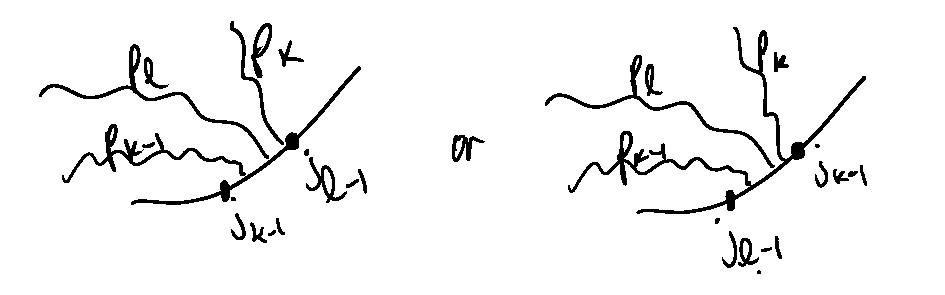
\includegraphics{induction_conf}
% \]
% If $p_\ell=p_1$ then $j_{\ell-1}=j_0$ and then as $j_0\not\in I_i$ but $p_r$ is supported at $j_0$ we get $I_i(p_r) <_i j_0$ and also $I_i(p_r) <_i j_{r-1} = J(p_r)$ as the only vertices not yet taken for $I_i(p_r)$ must be before both labelled vertices in the illustration.

% If $p_\ell \neq p_1$ then we argue as above with $\ell-1$ in place of $r-1$: in particular $J(p_\ell) = I_i(p_{\ell-1})$ but $p_r$ is supported at $p_{\ell-1}$, so either $I_i(p_r) <_i I_i(p_{\ell-1})$ in which case as before we get desired conclusion, or $p_r$ comes before $p_{\ell-1}$ at $j_{\ell-1}$.  Then again argue as before getting a new $p_{\ell'}$ in place of $p_{\ell}$, except that then case $(*)$ must occur simultaneously for both $p_{\ell'}$ and $p_{\ell}$ with respect to $p_{r}$.  This can only occur if $j_{\ell-1}, j_{r-1}, j_{\ell'-1}$ are consecutive.  Iterating the argument one more time we finally cannot have case $(*)$ as then all neighbouring vertices of $j_{r-1}$ are used up.

This covers all cases and completes the induction, and thence the proof of the theorem.

\end{proof}

\sanote{alternate proof of second half of above}
{\color{violet} \begin{thm}
The Grassmann necklace $(I_1 \ldots I_n)$ is the Grassmann neclace for $M(W)$ 
\end{thm}

\begin{proof}
We have shown that $(I_1,\dots,I_n)$ is a Grassmann necklace; it remains to check that this Grassmann necklace corresponds to the positroid $M(W)$.  Recall from the discussion following Definition~\ref{def:grassmann necklace}, and equation \eqref{basesofmatroids} in particular, that it suffices to show: 
\begin{itemize}
\item For each $i \in [n]$, $I_i$ is a basis for $M(W)$.
\item If $J$ is lexicographically smaller than $I_i$ with respect to $<_i$ (for any $i \in [n]$) then $J$ is not a basis for $M(W)$. 
\end{itemize}
The first point follows immediately: since the algorithm is pairing each $j \in I_i$ with a unique propagator supported on that vertex, $I_i$ is a basis for $M(W)$ by Corollary~\ref{lem basis as perm}.
 
For the second point, order the propagators according to the ordering induced by the algorithm for $I_i$. Write $\cP = \{p_1, \ldots , p_k\}$. That is, $p_i$ defines the $i^{th}$ row of $C(W)$. For $m<k$, write $\cP_m = \{p_1, \ldots , p_k\}$.

Write $I_i(p_j)=a_j$. If two consecutive propagators do not contribute consecutive vertices, that is, there exist $a_{j-1} <_i x <_i a_j$ then the vertex $x$ supports only propagators in $\cP_j$, if any: $\Prop(x) \subset \cP_j$. 

Let $J = (j_1,\ldots j_k)$ be a sequence that is lexicographically less than $I_i = (a_1 \ldots a_k)$: $J <_i I_i$. By the above, for some $m < k$, $a_{m-1} <_i j_m <_i a_m$ and the matrix entry $c_{m, j_m} = 0$ is $0$. Without loss of generality, let $m$ be the smallest $m$ in the $<_i$ order for which this is true: \bas \forall l <m, \; I_i(p_l) = j_l \; ; \; j_m < I_i(p_m) \;.\eas Write $J_m = (j_1, \ldots, j_m)$ indicate the first $m$ entries of $J$. We claim that there exists some subset  of vertices $U \subset J_m$ such that $|\Prop(U)| < |U|$. 

Consider the vertices contributed by the propagators originally supported on $j_m$: $V = I_i(\Prop(j_m))$. By construction, these are a subset of $J_{m-1}$. Note that $\Prop(V) \subset \cP_m$. Let $p_l$ be supported on $j_m$. If $q$ is suported on $p_l$, either $q$ preceeds $p_l$ (i.e. is not there when the algorithm reaches $a_l$) or is positioned counterclockwise to $p_l$ at the vertex $a_l$. That is, $q$ is inside $p_l$ in the $<_i$ ordering. By Lemma \ref{lem no fourth vertex}, $q$ does not contibute its last supporting vertex to $I_i$. That is, $I_i(q) <j_m$. \hlfix{But this implies that $q$ contributed before $p_m$, which contradicts the hypothesis.}{Seems to demand that $I_i$ catches all propagators in a single circuit of the vertices. Is this explicit anywhere, or am I jumping the gun?} Therefore $q \in \cP_{m-1}$.

If $\Prop(j_m) = \Prop(V)$, we have that $V$ and $V \cup j_m$ support the same propagators. That is, \bas |\Prop(V)| = |V| = |\Prop(V \cup j_m )| <  |V \cup j_m| \;.\eas

If $\Prop(j_m) \subsetneq \Prop(V)$, expand $V$ to include the vertices contributed by $\Prop(V)$. That is, $V' = I_i(\Prop(V))$. By the argument above, $\Prop(V) \subset \cP_m$. If $\Prop(V) = \Prop(V')$ then the relevant vertex set is $V'$. Else, continue expanding $V'$ in this manner until no new propagators are added. Since all of these sets of propagators are contained in $\cP_m$, which is finite, this process is finite. 

\begin{comment}
By algorithm \ref{alg:put GN on WLD}, $a_j$ is the smallest number in the $<_{a_{j-1}}$ ordering such that $c_{j, a_j} \neq 0$ (that is, is an indeterminant entry). Therefore, $p_m \not \in \Prop(j_m)$. In fact, no $q$ that follow $p_m$ in the ordering can be supported on $j_m$. Since $j_m < a_m$, the algorithm for $I_i$ checks this vertex before $a_m$.  If any propagator in $\cP \setminus \cP_{m-1}$ are supported on $j_m$, then this propapagator would preceed $p_m$, i.e. be an element of $\cP_{m-1}$. Therefore, the only non-zero entries in column $j_m$ of $C(W)$ lie in the first $m-1$ rows.

Therefore, $\Prop(j_m) \subset \cP_{m-1}$. Let $V =  V(\Prop(j_m)) \cap J_{m-1}$ be the vertices in $J_m$ supporting the propagators supported on $j_m$. That is, $V$ is contains the vertices contributed by $\Prop(j_m)$. So $|\Prop(j_m)| \leq |V|$. We show that $\Prop (V) \subset \Prop_{m-1}$. Suppose otherwise. Let $q \in \cP \setminus \cP_m$ be a propagators after $p_m$ and $p_l \in \Prop(j_m)$ a propagators before $p_m$ supported on $j_m$ such that both $q$ and $p_l$ are supported on $I_i(p_l)= a_l$. Since $p_l$ contributes $a_l$, it must be the clockwisemost propagator in $\cP \setminus \cP_{l-1}$ supported on $a_l$. In other words, $q \in \cP_{in}(p_l, <_{a_l-1})$ is inside $p_l$ in the $a_l-1$ order. Specifically, the last supporting vertex of $q$ is strictly less than $j_m$.  By Lemma \ref{lem no fourth vertex}, $q$ does not contibute its last supporting vertex to $I_i$. That is, $I_i(q) <j_m$. \hlfix{But this implies that $q$ contributed before $p_m$, which contradicts the hypothesis.}{Seems to demand that $I_i$ catches all propagators in a single circuit of the vertices. Is this explicit anywhere, or am I jumping the gun?}

By construction, this implies that $V \subset \Prop(j_m)$. But $V$ contains the vertices 
Since $J_{m-1}$ is independent, $V \subset J_{m-1}$ is too. Therefore, $|V| \leq |\Prop(V)| $. Since  $\Prop (V) \subset \cP_{m-1}$
***************
For the second point, consider the matrix $C(W)$ associated to the diagram $W$. Recall that $C(W)$ is only defined up to an ordering of the propoagators of $W$. Therefore order them according to the ordering induced by the algorithm for $I_i$. Write $\cP = \{p_1, \ldots , p_k\}$. That is, $p_i$ defines the $i^{th}$ row of $C(W)$. 

Write $I_i(p_j)=a_j$. By algorithm \ref{alg:put GN on WLD}, $a_j$ is the smallest number in the $<_{a_{j-1}}$ ordering such that $c_{j, a_j} \neq 0$ (that is, is an indeterminant entry). It is the first column in the $j^{th}$ row of $C(W)$ that is both non-zero and is greater than the index contributed by the previous propagator:  \bas \begin{bmatrix}\ddots & & & & & & \\ \ldots  & c_{j-1, a_{j-1}} & * & \ldots &  & & \\  \ldots  &* &0 & \ldots & 0 &c_{j, a_j} & \ldots \\ & & & & & & \ddots \end{bmatrix}  \eas

Let $J = (j_1,\ldots j_k)$ be a sequence that is lexicographically less than $I_i = (a_1 \ldots a_k)$: $J <_i I_i$. By the above, for some $m < k$, $j_m <_i a_m$ and the matrix entry $c_{m, j_m} = 0$ is $0$. Without loss of generality, let $m$ be the smallest $m$ in the $<_i$ order for which this is true: \bas \forall l <m, \; I_i(p_l) = j_l \; ; \; j_m < I_i(p_m) \;.\eas Write $J_m = (j_1, \ldots, j_m)$ indicate the first $m$ entries of $J$. 

We claim that the $j_m^{th}$ column of $C(W)$ is in the span of the columns indexed by $J_{m-1}$.

Since $J_{m-1}$ is an independent set in $C(W)$, row reduce the first $j_{m-1}$ columns of $C(W)$ to have $1$ in the $(r, j_r)$ position and $0$ to the right: \bas \begin{bmatrix}1 &0  &\ldots  & &  &0 \\  * & \ldots  & * & 1 & 0&\ldots \\    &\ddots &  &  &\ldots & 1 \\  *&* &* &\ldots &* &* \\  &\ddots & & & \ddots &  \\ *&* &* &\ldots &* &*  \end{bmatrix}  \;.\eas \sanote{fix this! wrote echelon order!}

Next consider the $j_m^{th}$ column of $C(W)$. First note that, since $c_{m, j_m} = 0$. Furthermore, no $q$ that follow $p_m$ in the ordering can be supported on $j_m$. Since $j_m < a_m$, the algorithm for $I_i$ checks this vertex before $a_m$.  If any propagators remain to be supported on this vertex after the removal of $p_1$ to $p_{m-1}$, then this propapagator would preceed $p_m$. Therefore, the only non-zero entries in column $j_m$ of $C(W)$ lie in the first $m-1$ rows.  \sanote{add something here} Therefore, column $j_m$ lies in the span of the first $j_{m-1}$ columns of $C(W)$. 

*******
%If $p, q \in \Prop(i)$ are two propagators supported on the vertex $i$, we may write $p = (a_p, b_p)$ and $q = (a_q, b_q)$, with the initial vertices $a_p$ and $a_q$ in the set $\{i, i-1\}$. By construction, the propagator $q$ is located clockwise relative to $p$ if and only if $p$ is inside $q$. That is, $p \in \cP_{in}(q, <_{a_q})$. 

%For $m < k$, write $\cP_m =\{p_1, \ldots , p_m\} \subset \cP$ to indicate the first $m$ propagators. For any subset of propagators $Q \subset \cP$, write $W|_Q = (Q, [n])$ be the subdiagram of $W$ consisting only of the propagators in $Q$ and all the vertices $[n]$.


%Since $p$ never contributes its last vertex in the $<_i$ order to $I_i$, by Lemma \ref{lem no fourth vertex}, every propagator preceeding $p_j$ is outside it in the $a_j-1$ ordering: $\cP_{j-1} \subset \cP_{out}(p_j)$. 


We claim that $J_m$ is not a basis for $W|_{\cP_m}$. To see this, first note that, since $c_{m, j_m} = 0$, the propagator $p_m$ is not supported on $j_m$. If $p_m$ does not share support with any propagator in $\cP_m$ in the cyclic interval $[i, j_m]$, then the minor of $C(W|_{\cP_m})$ defined by $J_{m}$, has a row of $0$s.

Otherwise, let $p_l$ be a propagator preceeding $p_m$ ($p_l \in \cP_{m-1}$) that shares support with it in $J_m$: $V(p_l) \cap V(p_m) \cap J_m \neq \emptyset$. Then $p_l \in Q$ is positioned clockwise to $p_m$ on vertex $a_l$, therefore, $p_l$ is outside $p_m$ in the $a_l -1$ order. Since $a_l <_i j_m <_i a_m$ with $a_l$ and $a_m$ both in the support of $p_m$, \hlfix{$j_m$ is inside $p_m$ in the $a_l-1$ ordering. }{I know we got rid or interior vertices. Can we bring it back or rephrase?} Furthermore since all of $\cP_{m-1} \subset \cP_{out}(p_m)$ is outside of $p_m$ in that $a_l-1$ order, and $j_m$ is a vertex inside it, no propagator prior to $p_m$ can be supported on $j_m$. Otherwise, one would have crossing propagators. Therefore, the minor of $C(W|_{\cP_m})$ defined by $J_{m}$, has a column of $0$s.
******
\end{comment}
\end{proof}
}


We can now unambiguously refer to Algorithm~\ref{alg:put GN on WLD} as the Grassmann necklace algorithm. We close this section with a simple observation about the Grassmann necklaces of positroids associated to Wilson loop diagrams.


In an arbitrary Grassmann necklace, it is possible for an index $i$ to appear in no terms of the Grassmann necklace (a {\em loop}) or in all terms of the necklace (a {\em coloop}). Using Theorem~\ref{res:alg gives GN}, a characterization of the loops and coloops of the Grassmann necklace associated to a Wilson loop diagram follows easily.


\begin{cor}\label{no coloops}\sanote{cite more prominently in frontmatter}
Grassmann necklaces coming from admissible Wilson loop diagrams have no coloops. A vertex $j$ is a loop if and only if $j$ supports no propagators. 
\end{cor}
\begin{proof}
For any $i \in [n]$, $i-1$ is maximal with respect to the $<_{i}$ order and so by Lemma~\ref{lem no fourth vertex} there can be no propagator $p$ with $I_{i}(p) = i-1$. Thus $i-1 \not\in I_{i}$, so $i-1$ is not a coloop. Since this holds for any $i \in [n]$, the Grassmann necklace admis no coloops.

If $j \in [n]$ is a loop then in particular we have $j \not\in I_j$, which can only happen if there are no propagators supported on vertex $j$. Conversely, if $j$ supports no propagators, then Algorithm~\ref{alg:put GN on WLD} never assigns a propagator to $j$ and hence $j \not\in I_i$ for all $i \in [n]$.
\end{proof}





\section{Dimension of the Wilson Loop cells}\label{sec dim}

Our next goal is to show that the dimension of the positroid cell defined by a Wilson loop diagram $(\cP, [n])$ has dimension $3|\cP|$ (Theorem \ref{thm dim}).  The positroid cells associated to the Amplituhedron are of dimension $4|\cP|$. In \cite{non-orientable}, Marcott and the first author show that the dimension of the Deodhar component is $|\cP| +$ the dimension of associated positroid cell. In otherwords, the Deodhar component associated to a Wilson loop diagram is $4|\cP|$, showing that the geometry underlying the Wilson loop diagrams is consistent with the geometry underlying the Amplituhedron.

Marcott in \hlfix{***cite this***}{highlighted for anyone skimming through} has a different proof of the dimension of the positroid cell assicated to a Wilson loop diagram, which is geometric and more elegant, but it is not easy to track the effect of a particular propagator.  Our approach is much more explicit.

Recall that the dimension of a positroid cell is equal to the number of plusses in the associated Le diagram \cite[Theorem 6.5]{Postnikov}. By combining Algorithms~\ref{alg:put GN on WLD} and \ref{alg:GN to Le} (converting from WLD to Grassmann necklace to Le diagram) we explicitly describe the effect of adding another propagator to a Wilson loop diagram in terms of the plusses of the associated Le diagrams, and hence give a recursive proof of the $3|\cP|$-dimensionality of the cells.

We start with several lemmas, of roughly increasing degree of technicality. Lemma \ref{lem uncovered} shows that non-supporting vertices corresopond to columns of $0$s in the associated Le diagram. The proof of Theorem \ref{thm dim} depends on being able to act on Wilson loop diagrams by elements of the dihedral group to position propagators in certain positions. Lemma \ref{lem dihedral} shows that the dihedral group action does not change the dimension of of the associated Le diagram.

\begin{lem}\label{lem uncovered}

Let $W$ be an admissible Wilson loop diagram with $k$ propagators, and with a vertex $i$ that supports no propagators.  Let $V$ be $W$ with vertex $i$ removed.  Then the Le diagram of $W$ is obtained from the Le diagram of $V$ by inserting an extra column containing all $0$s in position $i$ (i.e. such that the new column has the label $i$).
\end{lem} 

\begin{proof}
  By Algorithm~\ref{alg:put GN on WLD} the Grassmann necklace of $W$ is obtained from the Grassmann necklace of $V$ by duplicating the $i$th element of the Grassmann necklace of $V$ (shifting indices by $1$ for all indices greater than $i$), and incrementing all indices greater than $i$ by $1$ in each Grassmann necklace element.  Formally, if $I_1^{V}, \ldots, I_{n-1}^{V}$ and $I_1^{W}, \ldots, I_n^{W}$ are the Grassmann necklaces of $V$ and $W$ respectively then
  \[
  I_j^{W} =
  \begin{cases}
    \{\ell \in I_j^{V} : \ell < i\} \cup \{\ell+1 \in I_j^{V} : \ell \geq i\} & \text{if $j\leq i$} \\
    \{\ell \in I_{j-1}^{V} : \ell < i\} \cup \{\ell+1 \in I_{j-1}^{V} : \ell \geq i\} & \text{if $j > i$.}
  \end{cases}
  \]


By Lemma~\ref{no coloops} we know that $i \not\in I_1^W$, and so $i$ must label a horizontal edge on the boundary of the Le diagram of $W$, i.e. it must be a column label. The shapes of the Le diagram of $V$ and $W$ are the same except for the insertion of this column since $I_1^*$ is the same for $V$ and $W$ except for the incrementation of the indices $\geq i$ in the transition from the necklace for $V$ to the necklace for $W$. 
\end{proof}


\begin{lem}\label{lem dihedral}
If two Wilson loop diagrams differ by a dihedral transformation then their Le diagrams have same number of plusses.
\end{lem}
\begin{proof}
By \cite[Proposition 17.10]{Postnikov}, the dimension of a positroid (and hence the number of plusses in its Le diagram) is $k(n-k) - A(\pi_W)$, where $A(\pi_W)$ denotes the number of alignments of the decorated permutation $\pi_W$ of the positroid associated to $W$. (See \cite[Figure 17.1]{Postnikov} and preceding discussion.)

It can easily be seen from \cite[Section 17]{Postnikov} and Algorithm \ref{alg:put GN on WLD} that dihedral transformations of a Wilson loop diagram $W$ correspond to dihedral transformations of the chord diagram representation of $\pi_W$. Since the number of alignments in a chord diagram is preserved under dihedral transformations, the result follows.
\end{proof}


\begin{lem}\label{lem good p}
  Let $W$ be an admissible Wilson loop diagram with $n\geq 1$ propagators.  Then there is some dihedral transformation $W'$ of $W$ such that $W'$ has a propagator $p$ with the following properties.
  \begin{itemize}
  \item $p = (i, n-1)$ for some $i$, and $p$ has no propagators inside it w.r.t the $<_i$ ordering (that is $i+2, \ldots, n-2$ do not support any propagators in $W'$).
  \item Either the edge $i$ in $W'$ only supports $p$, or the edge $i$ in $W'$ supports exactly one other propagator $q = (j,i)$, with no other propagators inside $q$ in the $<_j$ ordering. \note{Sian undid Susama's change here: all we know about $q$ is that it goes from some edge $j$ to $i$, and there's nothing inside $q$ wrt that orientation. In a very degenerate case, $q$ could probably be $(n,i)$.}
  \end{itemize}
\end{lem}

\begin{proof}
  Remove all vertices of $W$ which do not support any propagators to get a weakly admissible Wilson loop diagram $V$.  Lemma~\ref{lem sian} applied to $V$ gives a length 2 propagator $p$ in $V$ for which either no other propagator is supported on one of the supporting edges of $p$ or there is a second length 2 propagator which is the only other propagator supported on one of the supporting edges of $p$.  (Figure~\ref{fig 3 cases} shows the possible configurations arising from Lemma~\ref{lem sian}, and the reader can easily check that in each case $p$ must be in one of the two situations described above.)

  We can now make a dihedral transformation of $V$ to obtain a diagram satisfying the statement of the lemma with $p$ and $q$ both length 2. Restoring the vertices which do not support any propagators, we obtain a dihedral transformation $W'$ of $W$ as desired (with potentially longer lengths for $p$ and $q$).
\end{proof}



Combining Lemmas \ref{lem uncovered}, \ref{lem dihedral}, and \ref{lem good p}, it therefore suffices to study the Le diagrams of weakly admissible Wilson loop diagrams with $F(\emptyset)  = \emptyset$, admitting one of the configurations described in Lemma \ref{lem good p} with propagators $p = (n-3, n-1)$ and $q= (n-5, n-3)$ (if $q$ exists) both of length 2. See Figure~\ref{fig special p} for an illustration of the two possibilities. 

The next few lemmas describe how diagrams of this type are related to the corresponding diagram with propagator $p$ removed, first in terms of the Grassmann necklaces (Lemma \ref{lem I}) and then in terms of the Le diagrams (Lemmas \ref{lem shape} to Lemma \ref{lem other k}) . These technical lemmas will form the backbone of the inductive step in the main dimensionality argument.

\begin{lem}\label{lem I}
Let $W$ be an admissible Wilson loop diagram with $n\geq 1$ propagators, and suppose that $W$ admits one of the configurations described in Lemma~\ref{lem good p}, with $p$ and $q$ (if $q$ exists) both of length 2. Let $V$ be $W$ with $p$ removed.  Then

  \begin{align*}
    I_1^{W} & = I_1^{V} \cup \{n-3\} \\
    I_n^{W} & = I_1^{V} \cup \{n\} \\
    I_{n-1}^{W} & = I_n^{V} \cup \{n-1\} \\
    I_{n-2}^{W} & =
    \begin{cases}
      I_{n-2}^{V}\cup \{n-2\} & \text{if $n-2\not\in I_{n-2}^{V}$} \\
      I_{n-2}^{V}\cup \{n-1\} & \text{if $n-2\in I_{n-2}^{V}$, $n-1\not\in I_{n-2}^{V}$} \\
      (I_{n}^{V} - \{n-5\})\cup \{n-1,n-2\} & \text{if $n-1, n-2\in I_{n-2}^{V}$}
    \end{cases} \\
    I_{k}^{W} & =
    \begin{cases}
      I_k^{V}\cup \{n-3\} & \qquad \qquad \qquad \qquad \text{if $n-3 \not\in I_k^{V}$}\\
      I_k^{V}\cup\{n-2\} & \qquad \qquad \qquad \qquad \text{if $n-3\in I_k^{V}$}
    \end{cases} \\
    & \text{for $1<k<n-2$}
  \end{align*}
\end{lem}

\begin{figure}
 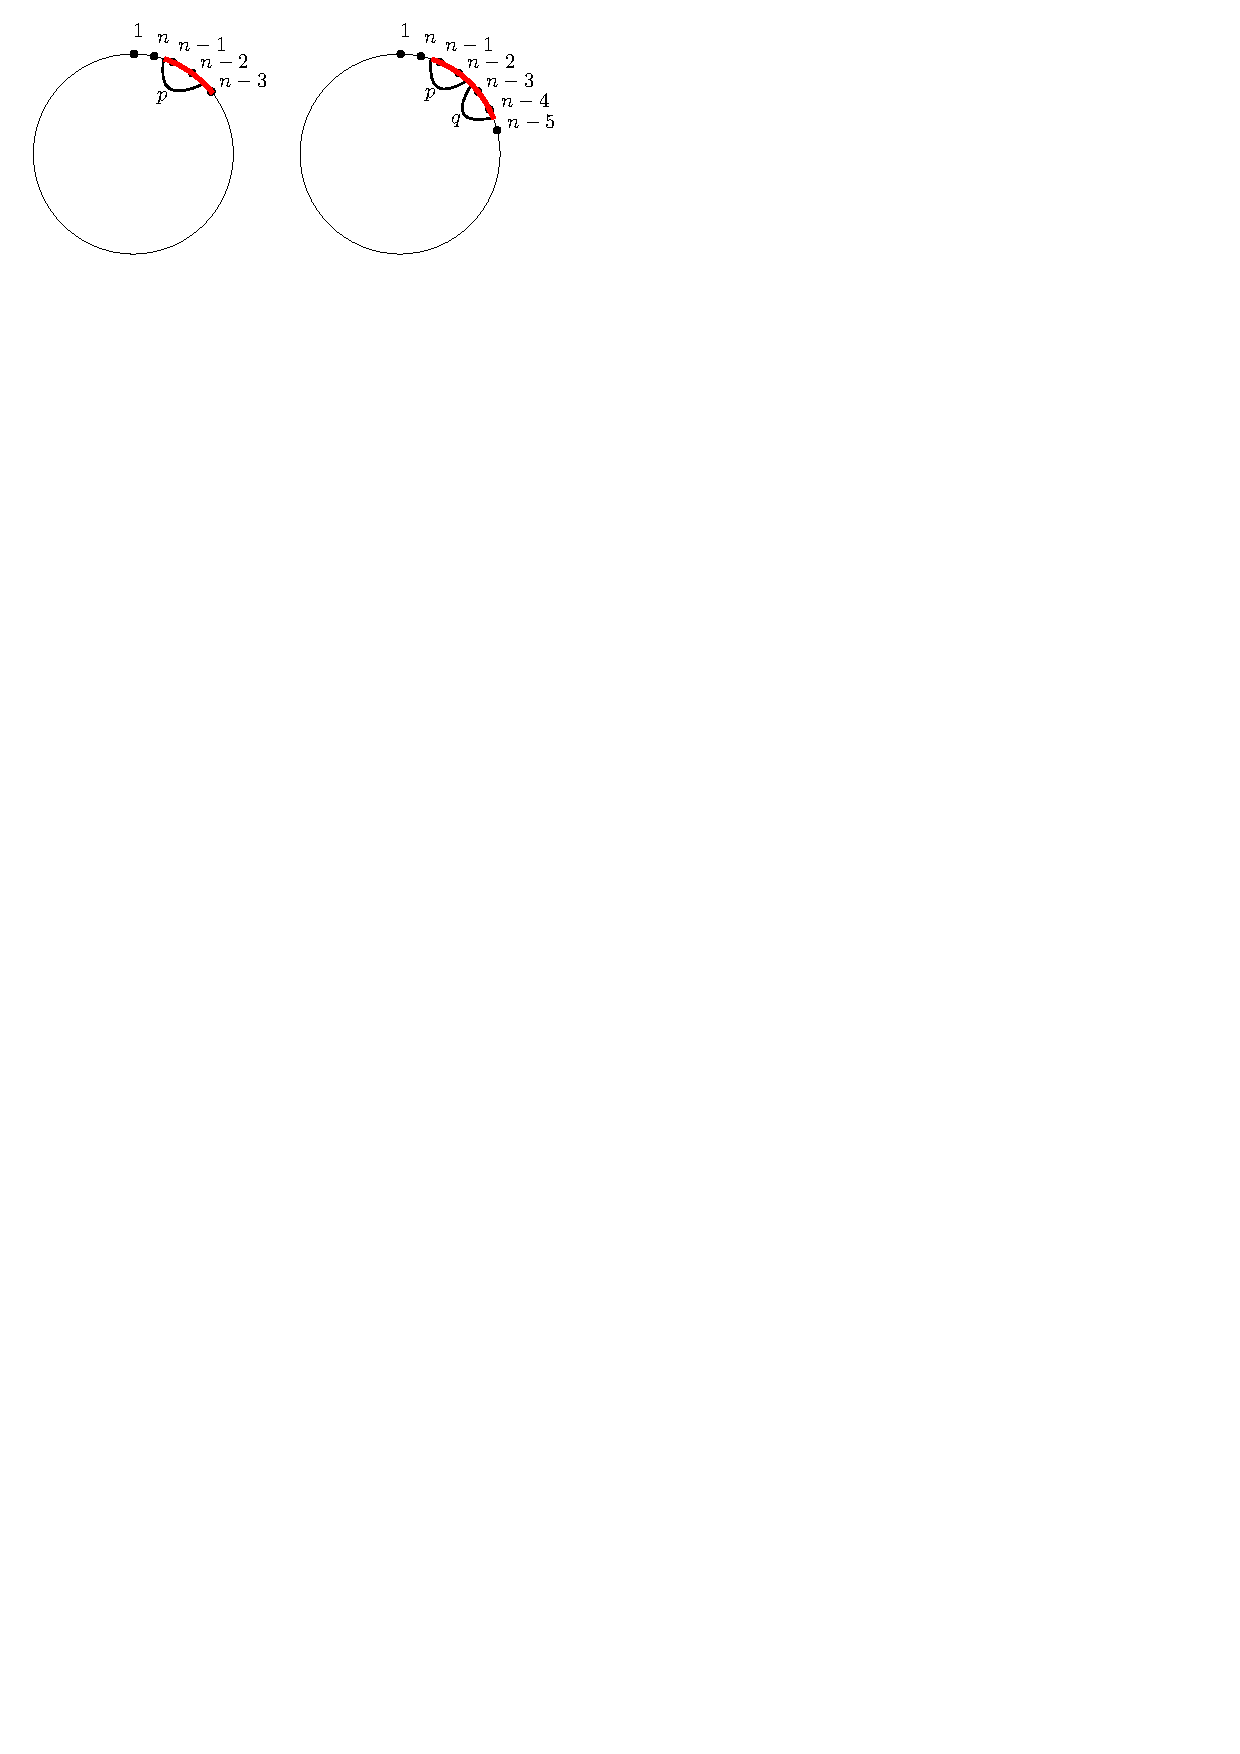
\includegraphics{specialp}
  \caption{The two cases for $W$ and $p$.  No other propagators can end in the fat red sections.  Other segments may have additional propagators ending in them.}\label{fig special p}
\end{figure}

\begin{proof}

The two possible cases for $W$ are illustrated in Figure~\ref{fig special p}; all references to the ``left hand case'' or ``right hand case'' below refer to the diagrams in this figure.

We first consider $I_1^{W}$, i.e. the set obtained by applying the Grassmann necklace algorithm to $W$ with starting vertex 1. Note that $n-3 \not\in I_1^{V}$: for the right hand case this is clear from the diagram (since Algorithm~\ref{alg:put GN on WLD} would assign $q$ no later than vertex $n-4$), while for the left hand case it follows from Lemma \ref{lem no fourth vertex}. Therefore when we start at vertex 1 and apply the Grassmann necklace algorithm to $W$, $p$ is the only remaining unassigned propagator when we reach vertex $n-3$, and so we have $ I_1^{W}(p) = n-3$ and $I_1^W = I_1^V\cup \{n-3\}$.


Next consider $I_n^{W}$. From the figure we see that in both cases we have $I_n^{W}(p) = n$. At vertex 1 of the algorithm $I_n$, the unassigned propagators are exactly those that appear in $V$. Therefore the algorithm continues as in $I_1^{V}$ (recall Remark~\ref{rmk algorithm locally same} about locally identical propagator configurations), i.e. we have $I_n^{W} = I_1^{V} \cup \{n\}$. By a similar argument, we must have $I_{n-1}^{W} = I_n^{V} \cup \{n-1\}$.

Now consider $I_{n-2}^{W}$. If $n-2\not\in I_{n-2}^{V}$ (i.e. $n-2$ supports no propagators in $V$), then $I_{n-2}^W(p) = n-2$ and this assignment of $p$ does not affect the rest of the construction of $I_{n-2}^{V}$, so we obtain $I_{n-2}^{W} = I_{n-2}^{V}\cup \{n-2\}$ as above.

On the other hand, if $n-2\in I_{n-2}^{V}$ then we must be in the right hand case of Figure~\ref{fig special p} and $I_{n-2}^V(q) = I_{n-2}^W(q) = n-2$ (since $q$ is always the clockwise-most propagator supported on vertex $n-2$; see Figure~\ref{fig special p}). If $n-1 \not\in I_{n-2}^{V}$, then $I_{n-2}^W(p) = n-1$ and then the algorithm proceeds identically to $I_{n-2}^{V}$ for the remainder of its steps; thus $I_{n-2}^{W} = I_{n-2}^{V}\cup \{n-1\}$ in this case.

Finally, if $n-2,n-1 \in I_{n-2}^{V}$ then $I_{n-2}^W(q) = n-2$ and $I_{n-2}^W(p) = n-1$ as above, but this is different to what occured in $I_{n-2}^{V}$ so we cannot use the same argument as above. When the algorithm $I_{n-2}^W$ reaches vertex $n$, the only propagators $p$ and $q$ have contributed; thus we proceed as in the construction of $I_n^{V}$ but without propagator $q$. By Lemma~\ref{vertex cyclic int lem} we know that $I_n^V(q) = n-5$, and from the diagram we see that the only way this could occur is if all other propagators in $V$ had already been assigned when we reached vertex $n-5$; thus $q$ was the final propagator to be assigned in $I_n^{V}$. Therefore $I_{n-2}^{W} = (I_{n}^{V} \setminus \{n-5\}) \cup \{n-1, n-2\}$ in this case. This completes all cases for $I_{n-2}^{W}$.

The arguments for $I_k^{W}$ ($1< k < n-2$) proceed analagously to those of $I_{n-2}^{W}$, with one simplification: we cannot have both $n-3$ and $n-2$ in $I_k^{V}$ since $q$ is the only propagator that could be assigned to either of them, and it cannot be assigned to both.

This covers all cases and hence completes the proof.
\end{proof}

\begin{figure}
  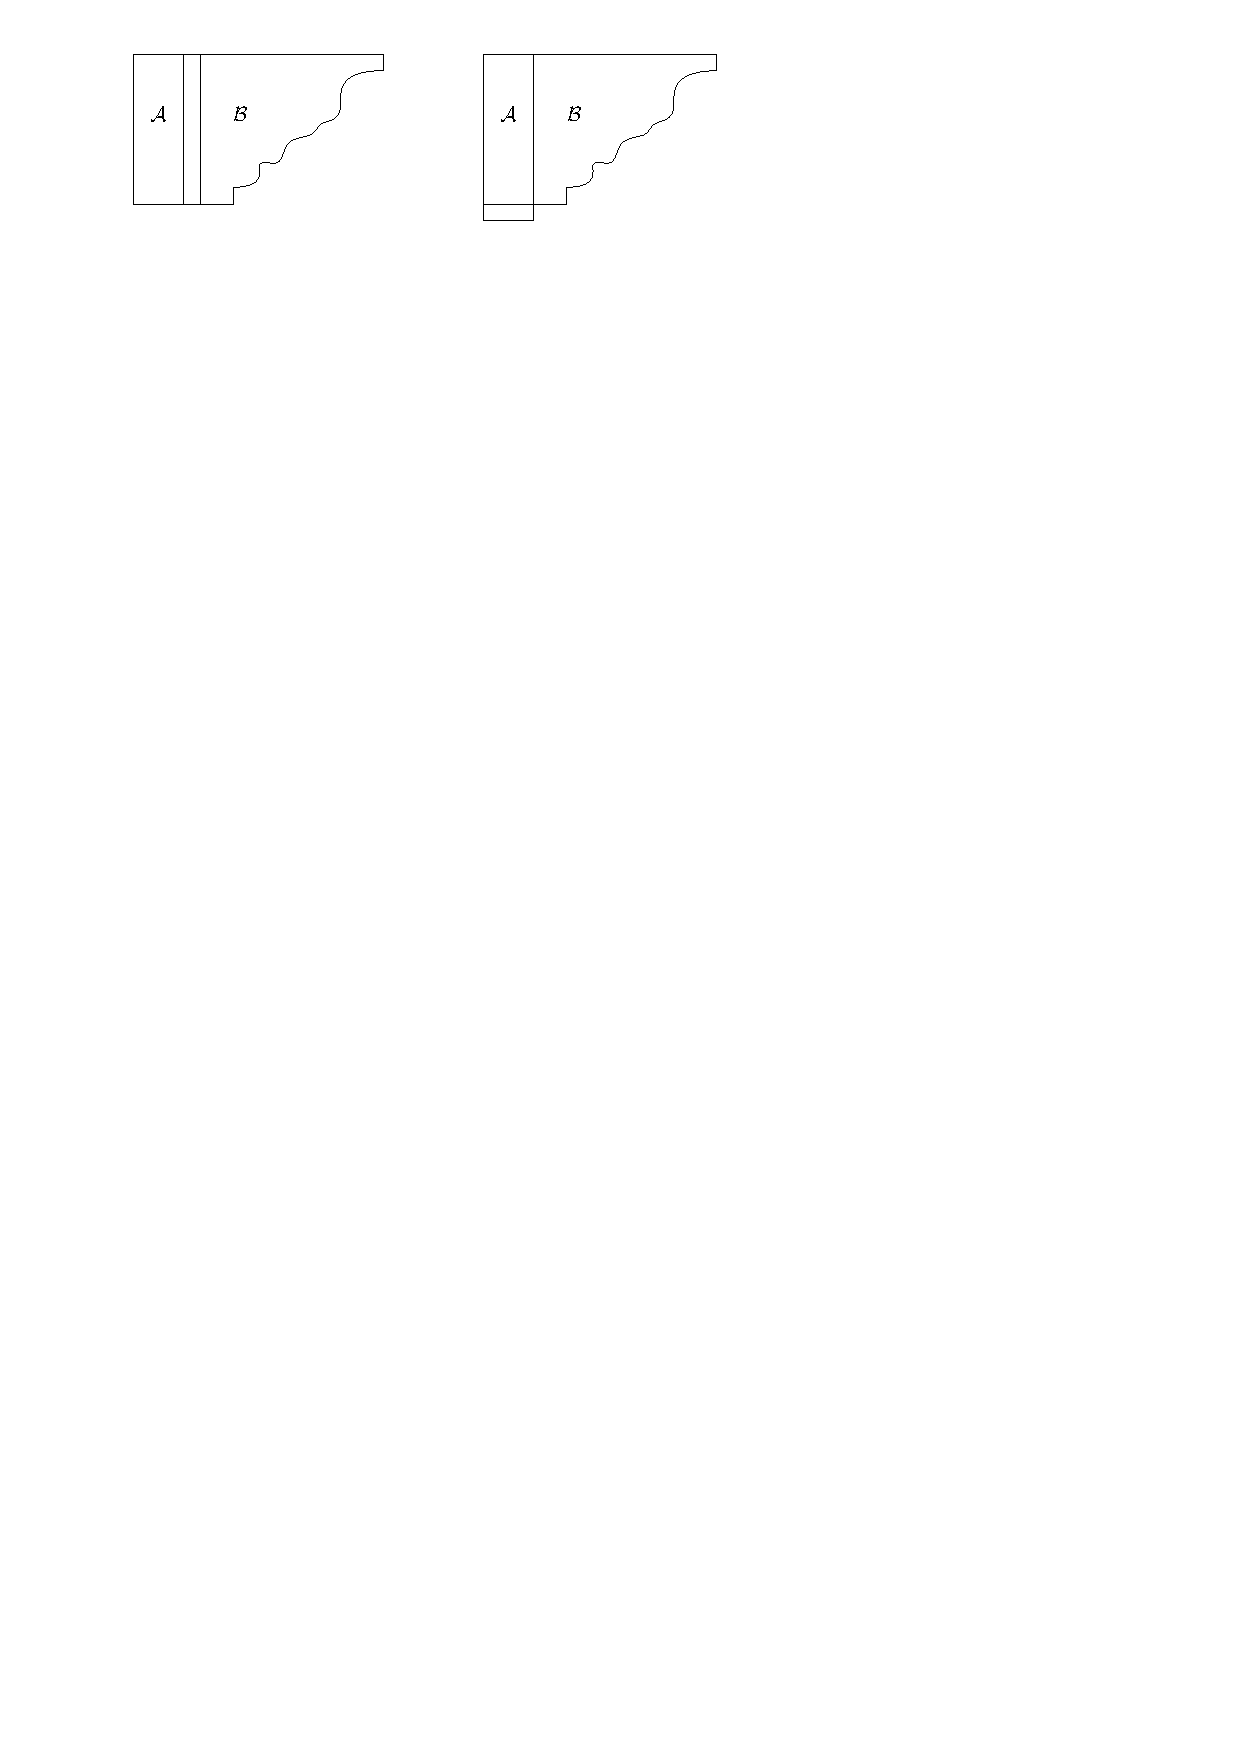
\includegraphics{Le_diagrams}
  \caption{Le diagrams for $V$ (left) and $W$ (right).}\label{fig Le}
\end{figure}

\note{When doing the final formatting, try to ensure that Figure \ref{fig Le} and Lemma \ref{lem shape} are on the same page}
\begin{lem}\label{lem shape}
  Let $V$ and $W$ be as in Lemma~\ref{lem I}.
  The shape of the Le diagram of $V$ can be built from left to right of the following blocks: a rectangle which is 3 columns wide, one more column of the same height, and a partition shape with at most as many rows as the rectangle.
  The shape of the Le diagram of $W$ can be built from left to right of the following blocks: a rectangle with 3 columns and one more row than the first rectangle of $V$, and the same partition shape as in $V$.
\end{lem}

\begin{proof}
See Figure~\ref{fig Le} for an illustration of the shapes described in the statement of the lemma.

Recall that $I_1$ determines the shape of the Le diagram: specifically, the elements of $I_1$ label the rows of the diagram, working from top right to bottom left. By the arguments in Lemma~\ref{lem I} we know that ${n,n-1,n-2, n-3 \not\in I_1^{V}}$ (which yields the leftmost four columns of the diagram for $V$) and that $I_1^{W} = I_1^{V}\cup \{n-3\}$. This implies that the right hand boundary of the shape of $V$ is the same as the right hand boundary of the shape of $W$ except that $W$ has one additional row of 3 boxes while $V$ has an additional column in the $n-3$ position; that is, an extra column fourth from the left. 
\end{proof}


As illustrated in Figure~\ref{fig Le}, the pieces of the Le diagrams of $V$ and $W$ will be called $\mathcal{A}$ and $\mathcal{B}$ in what follows. \hlfix{Explicitly, $\mathcal{B}$ is the set of columns with labels $v < n-3$ and $\mathcal{A}$ the set of columns labeled by $n$, $n-1$ and $n-2$ in $V$. In $W$, A consists of these columns without the last row.}{is this accurate?} Over the course of the next few lemmas we will prove that the plusses in the $\mathcal{B}$ parts of each diagram are identical, and that the relationship between the plusses in the $\mathcal{A}$ regions can be described explicitly.


We do this by applying Algorithm~\ref{alg:GN to Le}, which constructs the Le diagram associated to a Grassmann necklace, to the Grassmann necklaces of $V$ and $W$. As described in Section~\ref{sec:positroid background}, if Algorithm~\ref{alg:GN to Le} places a $+$ in the box with row index $i$ and column index $j$, we say that this plus is in the $i \rightarrow j$ position, and refer to it as the plus defined by ``the (hook) path from $i$ to $j$''. Note that the collection of paths contributed by a single Grassmann necklace term  must be non-crossing.



Finally, we also note that when we speak of a plus in the Le diagram of $V$ being the same as in $W$ or vice versa, we mean that the position of the plus in $\mathcal{A}$ or $\mathcal{B}$ is the same; because of the column insertion the absolute indices may differ.




\begin{lem}\label{lem n and n-1}
Let $V$ and $W$ be as in Lemma~\ref{lem I}.
Then $I_n^{W}$ and $I_{n-1}^{W}$ together yield the same plusses as $I_n^{V}$ did, along with two extra plusses which appear in the leftmost two boxes of the bottom row of the Le diagram of $W$.
\end{lem}

\begin{proof}
By Lemma~\ref{lem I} we have $I_n^{W}= I_1^{V} \cup \{n\}$ and $I_1^{W} = I_1^{V} \cup \{n-3\}$. Thus 
\[I_1^{W} \setminus I_n^{W} = \{n-3\}, \qquad \qquad I_n^{W} \setminus I_1^{W} = \{n\},\]
and so by Algorithm~\ref{alg:GN to Le} we have a plus in the $(n-3) \rightarrow n$ position, i.e. in the leftmost box of the bottom row. 

Also by Lemma~\ref{lem I} we have $I_{n-1}^{W} = I_n^{V} \cup \{n-1\}$. Recall from the proof of Lemma~\ref{lem I} that $n-3,n-2,n-1,n \not\in I_1^V$; therefore $I_1^W\setminus I_{n-1}^W = (I_1^V \setminus I_n^V) \cup\{n-3\}$, and $n-3$ is maximal in this set. Similarly, 
\[I_{n-1}^W \setminus I_1^W = (I_n^V \setminus I_1^V) \cup \{n-1\} \subseteq \{n-1,n\},\]
where the final inclusion follows from the definition of Grassmann necklace. In particular, $n-1$ is minimal in this set, so Algorithm~\ref{alg:GN to Le} yields a plus in the $(n-3) \rightarrow (n-1)$ position (i.e. the second box in the bottom row of the Le diagram of $W$) along with any plusses yielded by $I_n^V$.
\end{proof} 



\begin{lem}\label{lem n-2 good}
  Let $V$ and $W$ be as in Lemma~\ref{lem I}, and suppose that $n-2 \not\in I_{n-2}^{V}$. Then $I_{n-2}^{W}$ contributes all of the same plusses as $I_{n-1}^{V}=I_{n-2}^{V}$, along with a new $(n-3)\rightarrow (n-2)$ plus.
\end{lem}

\begin{proof}
If $n-2\not\in I_{n-2}^{V}$ then $I_{n-1}^{V}=I_{n-2}^{V}$ by definition, and by Lemma~\ref{lem I} we have $I_{n-2}^{W} = I_{n-1}^{V} \cup \{n-2\}$.  Note that $n-3\not\in I_{n-2}^{V}$ by Lemma~\ref{lem no fourth vertex}.  Therefore the paths controlling the plusses contributed by $I_{n-2}^{W}$ are exactly the paths for $I_{n-1}^{V}$ along with the $(n-3)\rightarrow (n-2)$ path.  This gives the statement of the lemma.
\end{proof}


\begin{lem}\label{lem n-2 bad}
Let $V$ and $W$ be as in Lemma~\ref{lem I}, and suppose that $n-2,n-1 \in I_{n-2}^{V}$. Then:
  \begin{enumerate}
  \item $I_{n-2}^W$ contributes an $(n-3)\rightarrow (n-2)$ plus and an $(n-5)\rightarrow (n-1)$ plus, along with any plusses contributed by $I_n^V$.
  \item $I_{n-3}^W$ contributes the same plusses as $I_{n-3}^V$, except that the plus in the $n-3$ column (which necessarily exists) is shifted one square left into the $n-2$ column.
  \item In the Le diagram of $V$, $I_{n-2}^{V}$ contributes an $(n-5)\rightarrow (n-2)$ plus and no other term in the Grassmann necklace of $V$ gives a plus in this column.  $I_{n-2}^W$ does not contribute this $+$ but yields the $(n-5)\rightarrow (n-1)$ plus from point (1) instead.
  \item All other plusses from $I_{n-2}^{V}$ and all plusses from $I_{n-1}^V$ were already contributed by $I_{n-3}^V$, so they yield no new information.
  \item No element of the Grassmann necklace of $V$ contributes a $(n-5)\rightarrow (n-1)$ plus.
  \end{enumerate} 
\end{lem}

\begin{proof}
  By Lemma~\ref{lem I} we have $I_{n-2}^{W}= (I_{n}^{V} \setminus \{n-5\})\cup \{n-1,n-2\}$ and $I_1^W = I_1^V\cup \{n-3\}$. We are necessarily in the case where $W$ admits a propagator $q$ (the right hand case of Figure~\ref{fig special p}) and we can see from the location of $q$ that $n-2\not\in I_{n-3}^{V}$ and that $n-5$ is the label of the last row in $\mathcal{B}$.  Also note that by Lemma~\ref{vertex cyclic int lem} and Corollary~\ref{no coloops} we must have $n\in I_n^V$. Thus this section of the Grassmann necklace of $V$ looks like

  \begin{equation}\label{eq necklace}
  I_{n-3}^{V} \xrightarrow[\substack{n-3\text{ out}\\n-2\text{ in}}]{} I_{n-2}^{V} \xrightarrow[\substack{n-2\text{ out}\\n-5\text{ in}}]{} I_{n-1}^{V} \xrightarrow[\substack{n-1\text{ out}\\\text{something in}}]{} I_{n}^{V}  \xrightarrow[\substack{n \text{ out}\\\text{something in}}]{} I_1^{V}
  \end{equation}
  where the first ``something'' is either $n$ or an element of $I_1^{V}$, and the second ``something'' is an element of $I_1^{V}$.

  \begin{figure}
    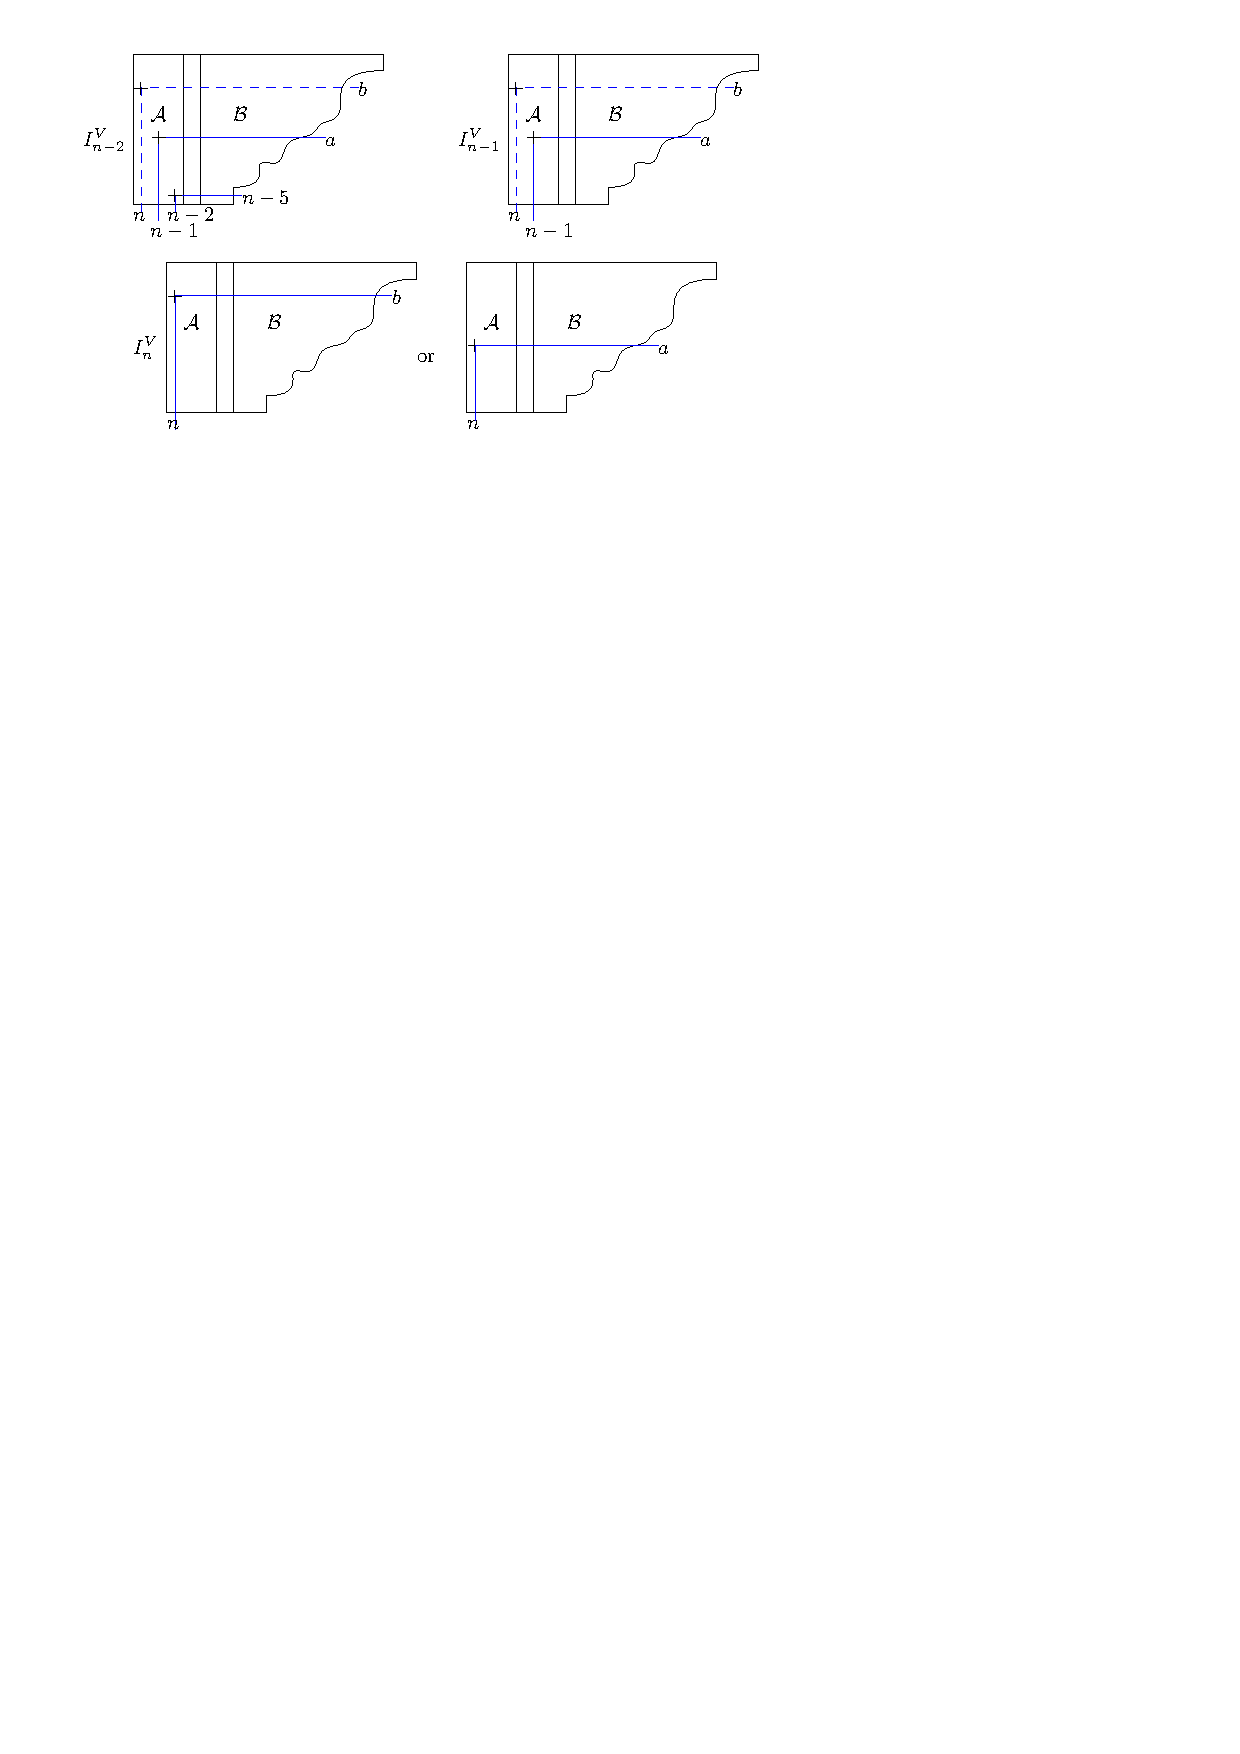
\includegraphics{messy}
    \caption{Plusses coming from $I_{n-2}^{V}$ (left) and  $I_{n-1}^{V}$ (right), in the case where $n-1, n-2\in I_{n-2}^{V}$.  The blue lines are the non-intersecting paths defining the position of the plusses.  The dashed blue lines may or may not appear, but if one appears then they both do.}\label{fig messy}
  \end{figure}
  
  Using this information we can determine the symmetric difference of $I_{n-2}^{V}$ and $I_1^{V}$.  Note that $I_{n-2}^V\setminus I_1^V$ and $I_1^V\setminus I_{n-2}^V$ each have size $\leq 3$ by the definition of a Grassmann necklace. We have $n-1, n-2 \in I_{n-2}^{V} \setminus I_1^V$ for certain, and the third element (if it exists) must be $n$. On the other hand we have $n-5 \in I_1^{V} \setminus I_{n-2}^V$, along with at least one and at most two other elements.  If there is one such element call it $a$.  If there are two call them $a$ and $b$ with $a>b$.  

  This means that the plusses in the Le diagram of $V$ coming from $I_{n-2}^{V}$ are as in the first part of Figure~\ref{fig messy}.  Stepping to $I_{n-1}^{V}$ simply removes the $(n-5)\rightarrow (n-2)$ path (second part of Figure~\ref{fig messy}), so $I_{n-1}^V$ contributes no new information about the Le diagram of $V$.

  %Stepping to $I_{n}^{V}$, $n-1$ is removed and either $n$ is put in if it was not there before, or one of $a$ or $b$ is put in and hence is no longer available as the starting point for a path.  This gives two possible configurations illustrated in the bottom two parts of Figure~\ref{fig messy}.

  With this information in hand, we can now tackle the points in the statement of the lemma. We know that 
  \[I_{n-2}^{W}  = (I_{n}^{V} - \{n-5\})\cup \{n-1,n-2\}, \quad n-5 \in I_1^W, \quad n-3\not\in I_{n-2}^W,\]
 and so the paths for building plusses from $I_{n-2}^{W}$ start at
 \[I_1^W \setminus I_{n-2}^W = \{n-3,n-5\} \cup (I_1^V \setminus I_n^V)\]
 and end at
 \[I_{n-2}^W \setminus I_1^W = \{n-2,n-1\}\cup(I_n^V \setminus I_1^V).\]
This means that $I_{n-2}^W$ contributes plusses as in Figure~\ref{fig messyD}, while $I_n^V$ contributes as in the bottom line of Figure~\ref{fig messy}, which proves point (1) and most of point (3). From equation \eqref{eq necklace} we see that $n-2$ appears only in $I_{n-2}^V$, so no other Grassmann necklace term for $V$ can contribute a plus in the $n-2$ column; this completes the proof of item (3).

  \begin{figure}
     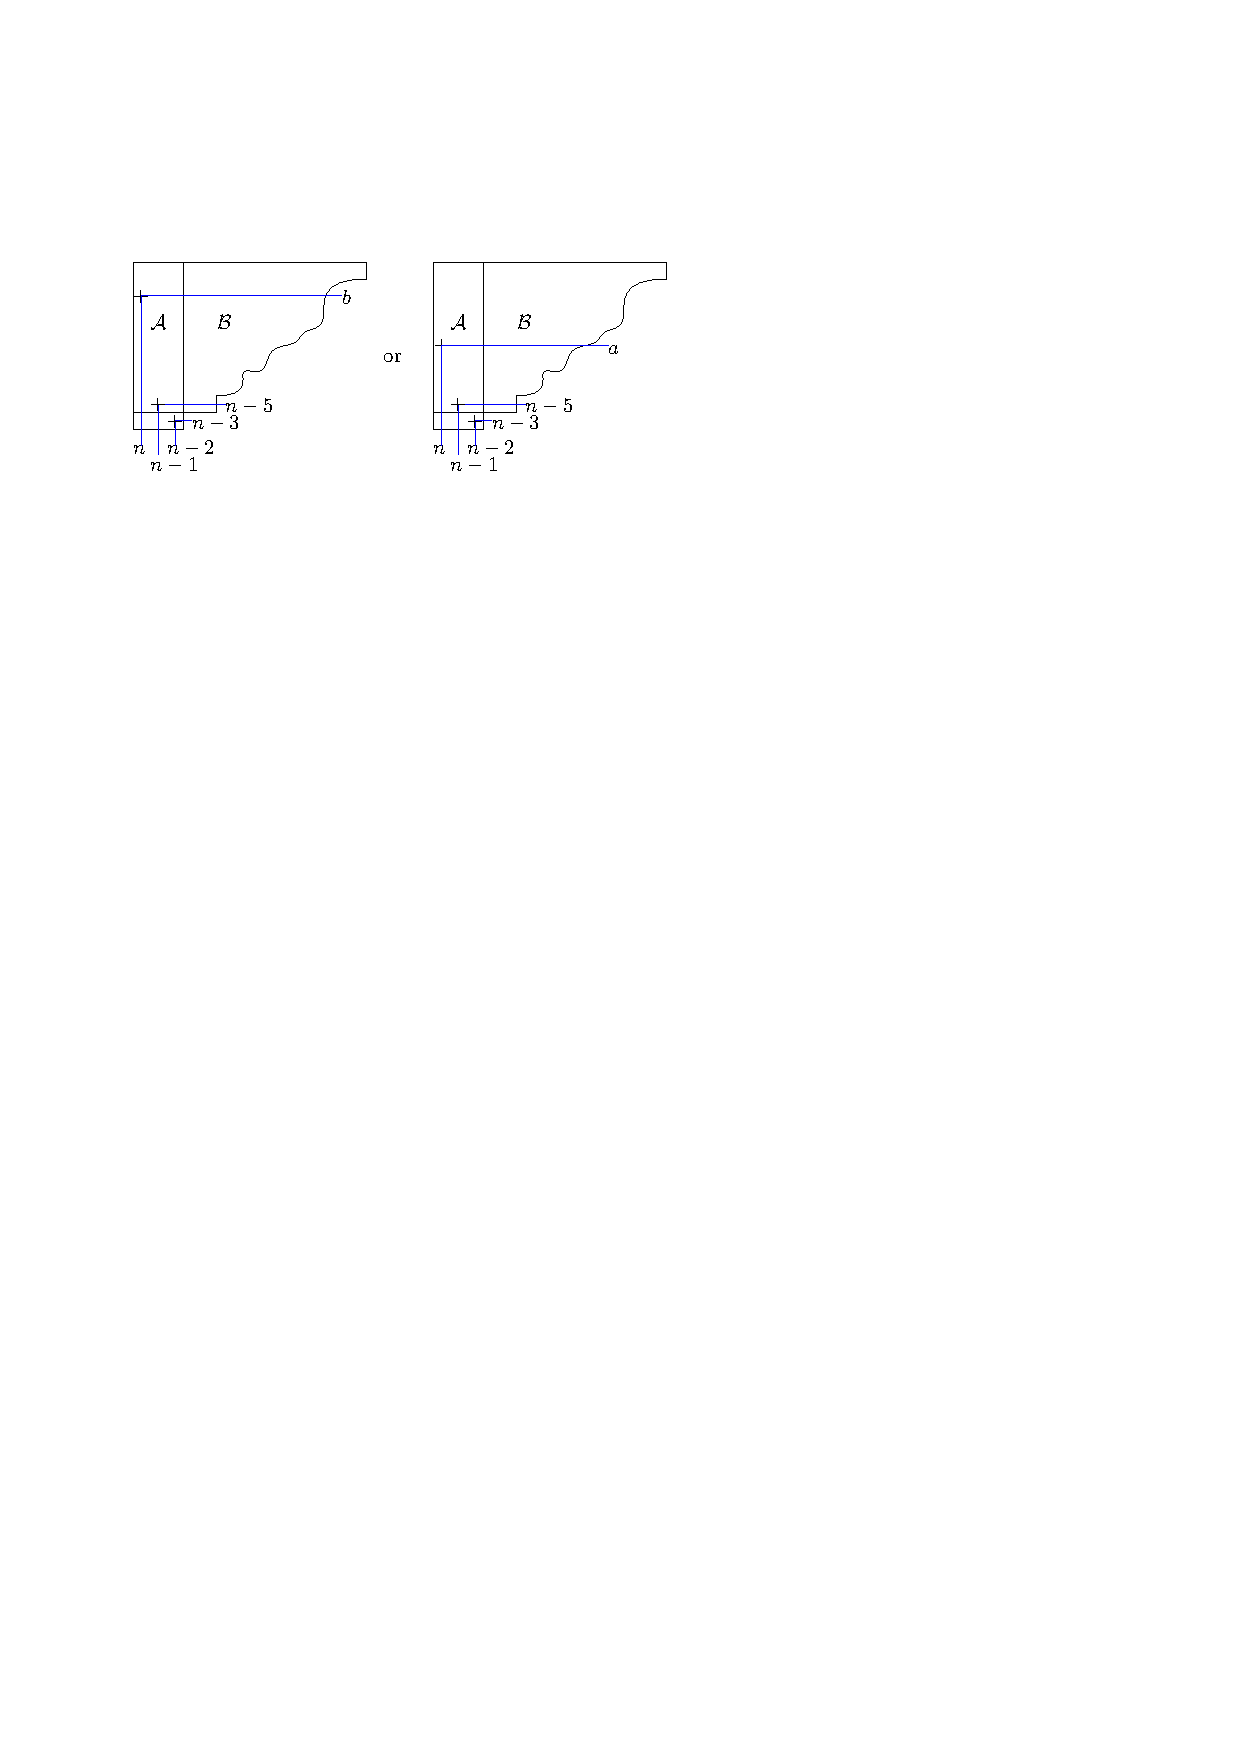
\includegraphics{messyD}
    \caption{Plusses coming from $I_{n-2}^{W}$.}\label{fig messyD}
  \end{figure}

Now consider $I_{n-3}^{V}$.  By \eqref{eq necklace} $I_{n-3}^{V}$ contributes almost the same plusses as $I_{n-2}^{V}$: the only difference is that it contributes an $(n-5)\rightarrow (n-3)$ plus in place of the $(n-5)\rightarrow (n-2)$ plus.  Since we must have $n-3\in I_{n-3}^{V}$ (because the propagator $q$ exists in $V$), it follows from Lemma~\ref{lem I} that $I_{n-3}^{W} = I_{n-3}^{V}\cup\{n-2\}$.  Thus the paths for $I^{W}_{n-3}$ are the same as those for $I^{V}_{n-3}$ except that the path that did go to $n-3$ now goes to $n-2$.  This cannot conflict with another path since \eqref{eq necklace} shows that $n-2$ only appears in $I_{n-2}^{V}$ among the necklace elements of $V$.

This proves point (2), and combined with the observation above that $I_{n-1}^V$ contributes no new plusses compared to $I_{n-2}^V$, we also obtain item (4).


  Finally, if the Le diagram of $V$ did admit a $(n-5)\rightarrow (n-1)$ plus, it could only have been contributed by a necklace term that doesn't contain $n-5$.  By equation \eqref{eq necklace} the only terms that could have this property are $I_{n-2}^{V}$, $I_{n-3}^{V}$, and $I_{n-4}^{V}$, and the analysis above shows that $I_{n-2}^V$ and $I_{n-3}^V$ do not contribute a plus in this position.

  Recall that $n-5$ is the largest row index in the Le diagram of $V$, and $n-5 \in I_1^V \setminus I_{n-4}^V$ so $I_{n-4}^V$ does contribute a path starting at $n-5$. Since $n-4 \in I_{n-4}^V$ by the location of the propagator $q$, we must also have a path ending at $n-4$. Since the paths cannot cross, this implies that $I_{n-4}^V$ must contribute a $(n-5) \rightarrow (n-4)$ plus, and hence cannot contribute a $(n-5)\rightarrow (n-1)$ plus. This proves point (5) and completes the proof of the lemma.
\end{proof}


\begin{lem}\label{lem other k}
  Let $V$ and $W$ be as in Lemma~\ref{lem I}, and suppose that if $n-2\in I_{n-2}^{V}$ then $n-1\in I_{n-2}^{V}$ also. Then for each $k$ in the range $1<k<n-2$, $I_k^{W}$ contributes the same plusses as $I_{k}^{V}$, except that if $I_{k}^{V}$ contributed a plus in the $n-3$ column of the Le diagram of $V$ then this plus is shifted one square left in the Le diagram of $W$, and no plus was already in that location in the Le diagram of $W$.
\end{lem}

\begin{proof}
Recall that $I_1^W = I_1^V\cup \{n-3\}$ and that $n-2,n-1,n \not\in I_1^W$.

  If $n-3\not\in I_{k}^{V}$ then by Lemma~\ref{lem I} we have $I_{k}^{W} = I_k^{V}\cup \{n-3\}$.  Then since $n-3$ is the largest element of $I_1^{W}$ this transformation leaves the disjoint paths unchanged and so the plusses carry over from $V$ to $W$ directly.

  If $n-3\in I_{k}^{V}$ then $I_k^V$ must contribute a plus in the $n-3$ column of the Le diagram of $V$, and by Lemma~\ref{lem I} we have $I_{k}^{W} = I_k^{V}\cup \{n-2\}$. If $n-2$ supports no propagators in $V$ then certainly no pluses appear in the $n-2$ column of the Le diagram of $V$. If $n-2$ supports at least one propagator in $V$ then $n-2 \in I_{n-2}^V$ and so by hypothesis $n-1 \in I_{n-2}^V$ as well. By Lemma~\ref{lem n-2 bad}, the only necklace element of $V$ containing $n-2$ is $I_{n-2}^{V}$ and the corresponding plus is not contributed to the Le diagram of $W$ by $I_{n-2}^{W}$.

  Since $n-3 \in I_k^V \setminus I_1^V$, we must have a path from some vertical edge $i$ to the bottom edge $n-3$ in the Le diagram of $V$.  In the Le diagram of $W$, the index $n-3$ labels a vertical edge with no path starting at it (since $n-3$ belongs to both $I_1^W$ and $I_k^W$), and there must be a path leading to $n-2$ since $n-2 \in I_k^W \setminus I_1^W$.  By the previous paragraph no other path from $I_k^V$ could end at $n-2$, and since the paths cannot cross we conclude that the $i\rightarrow (n-3)$ path in the Le diagram of $V$ must become a $i\rightarrow (n-2)$ path in the Le diagram of $W$. All other paths are unchanged.

   Thus the plus contributed by $I_k^V$ in the $n-3$ column of the Le diagram of $V$ is shifted into the $n-2$ column in the Le diagram for $W$, where there was no plus before, and no other plusses are changed.
\end{proof}

We are now ready to prove the main result of this section, showing that the dimension of the positroid cell associated to each Wilson loop diagram is $3|\cP|$. 

\begin{thm}\label{thm dim}
  The number of plusses in the Le diagram of an admissible Wilson loop diagram is three times the number of propagators.
\end{thm}

\begin{proof}
  The proof is by induction on the number of propagators.

  First note that a Wilson loop diagram $W$ with one propagator supported on vertices $i<j<k<\ell$ has Le diagram a single row with $|W|-i$ boxes.  Labelling the columns from left to right by $|W|, \ldots, |W|-i+1$, by the algorithm there are plusses in the $j$, $k$, and $\ell$ positions.

  Now consider Wilson loop diagrams with $k>1$ propagators.  By Lemma~\ref{lem uncovered} it suffices to prove the result for weakly admissible Wilson loop diagrams with $k$ propagators and no non-supporting vertices.  By Lemma~\ref{lem dihedral} it suffices to prove the result for at least one Wilson loop diagram from each dihedral orbit.  Take a weakly admissible Wilson loop diagram $W$ with $k$ propagators and no non-supporting vertices.  Make a dihedral transformation of $W$ if necessary so that $W$ has a propagator $p$ with the properties in Lemma~\ref{lem good p}.  

  We make one further simplification: if our $W$ is in Case 2 of Figure~\ref{fig special p} and $n-1$ supports only $p$ but $n-2$ supports at least one other propagator, then flip $W$ on the line perpendicular to the $(n-2)^{th}$ edge to obtain a diagram with the configuration of Case 1. This eliminates the possibility that we could have $n-2 \in I_{n-2}^W$ but $n-1 \not\in I_{n-2}^W$. 

  This diagram will be our $W$ for the remainder of the proof. Let $V$ be $W$ with $p$ removed. 

  From Lemma~\ref{lem shape} we know how the shapes of the Le diagrams of $V$ and $W$ are related; let $\mathcal{A}$ and $\mathcal{B}$ be as described above.  Lemmas~\ref{lem n and n-1}, \ref{lem n-2 good}, and \ref{lem n-2 bad} tell us that the three boxes of the bottom row of the Le diagram of $W$ each have a plus.  Lemmas~\ref{lem n and n-1} through \ref{lem other k} show that there is a bijection between the plusses of the Le diagram of $V$ and the plusses of the Le diagram of $W$ that are not in the bottom row.  This bijection can be described as follows:
  \begin{itemize}
  \item All plusses from $\mathcal{B}$ for $V$ maintain their positions in $\mathcal{B}$ for $W$.
  \item All plusses from the leftmost two columns (the $n$ and the $n-1$ columns) of $\mathcal{A}$ for $V$ maintain their positions in $\mathcal{A}$ for $W$.
  \item If there is a plus in the $n-2$ column of $\mathcal{A}$ in $V$ then Lemma~\ref{lem n-2 bad} applies, so there is exactly one such plus.  This plus is mapped to the $(n-5)\rightarrow (n-1)$ plus for $W$.
  \item All plusses in the $n-3$ column for $V$ are shifted one square to the left in $\mathcal{A}$ for $W$, i.e. into the $n-2$ column.
  \end{itemize}
  Note that this map is reversible and hence bijective. Indeed, the only possible ambiguity is at the $(n-5)\rightarrow (n-1)$ plus in $W$ (if it exists), which could have come from either of the first or third bullet points. However, if the third bullet point applies then by Lemma~\ref{lem n-2 bad} there is no $(n-5)\rightarrow (n-1)$ plus in $V$, i.e. the first bullet point does not apply. 



  % If the Le diagram for $V$ has a plus in the $n-2$ column then Lemma~\ref{lem n-2 bad} applies. By the final part of Lemma~\ref{lem n-2 bad} there is no $n-5\rightarrow n-1$ plus in the Le diagram of $V$, and so the $n-5\rightarrow n-1$ plus of $W$ can be uniquely mapped to the plus in the $n-2$ column of the Le diagram of $V$.  If the Le diagram for $V$ has no plus in the $n-2$ column, then leave the $n-5\rightarrow n-1$ plus where it is in moving back to $V$.  This reverses the map.

Therefore the Le diagram of $W$ contains $3(k-1)$ plusses in bijection with the plusses from the Le diagram of $V$ and 3 new plusses in the bottom row, yielding $3k$ in total. Applying induction completes the proof.
\end{proof}



\section{Poles of Wilson Loop Integrals}\label{sec poles}

In this section, we investigate the poles of the integrand for $I(W)$, that is $R(W)$ as defined in Definition~\ref{def R(W)}. It is conjectured that for a fixed number of propagators and a given set of external twistors $\cZ$, [cite] \bas \sum_{W | |\cP| = k} I(W)(\cZ) <\infty \;.\eas In otherwords, all poles of the intergrals must cancel. As a step towards this, in this section, we prove some results about $R(W)$.

The results of Section~\ref{sec GN algorithm} allow us to relate the position of propagators in a Wilson loop diagram $W$ to minors of $C(W)$, $R(W)$.

The main result of this section is Theorem~\ref{thm denom}, which expresses the denominator $R(W)$ in terms of the Grassmann necklace of $W$. This simplifies the computation of $R(W)$ and allows us to directly relate the poles of the integral to the combinatorics of the diagram.

We first give an algorithm which extracts the required minors from the Grassmann necklace. 


\begin{algorithm}\label{alg WLD to denom via GN}
Let $W = (\cP,n)$ be a Wilson loop diagram, and let $C(W)$ be the matrix of $W$ as defined in \eqref{C(W) dfn} with a fixed ordering on $\cP$. (see Section~\ref{section WLD background}).
\begin{itemize}
  \item For each $i \in [n]$, we construct a factor $r_i$ as follows:
    \begin{itemize}
      %\item Use Algorithm~\ref{alg:put GN on WLD} to obtain a bijection between the propagators and the $i-1$st Grassmann necklace element, $I_{i-1}$.  (By convention set $I_{-1}=I_n$.)  Write $I_{i-1}(p)$ for the vertex associated to propagator $p$ under this bijection.
      %\item Use Algorithm~\ref{alg:put GN on WLD} to obtain a bijection between the propagators and the $i$th Grassmann necklace element, $I_{i}$.  Write $I_{i}(p)$ for the vertex associated to propagator $p$ under this bijection.
      \item Let $S_i = \{p \in \cP \ | \ I_{i-1}(p) \neq I_i(p)\}$. (By convention, set \hlfix{$I_{0} = I_n$}{changed. correct?}.)
	  %\item Write $\Delta_{I_i}$ for the determinant of the $k \times k$ minor of $C(W)$ with columns indexed by $I_i$.
      \item Let $r_i$ be the determinant of the $|S_i|\times |S_i|$ minor of $C(W)$ with rows indexed by $S_i$ and columns indexed by $I_i(S_i)$.  %$\Delta_{I_i}$ with all variables from rows associated to $p\not\in S_i$ set to $1$.
    \end{itemize}
  \item Define $R = \prod_{i=1}^n r_i$.
\end{itemize}
\end{algorithm}

\hlfix{That is, each $r_i$ is the determinant of the minor determined by the propagators (rows) that contribute different values (columns) to the $i^{th}$ element of the Grassmann necklace than they did to the $i-1^{th}$.}{added. accurate?}


As we discuss the algorithm it will also be useful to have the notation $\Delta_{I_i}$ for the determinant of the $k\times k$ minor of $C(W)$ with columned indexed by $I_i$.

As we take each $r_i$ to simply be the determinant of a particular submatrix of $C(W)$, the sign of each $r_i$ is well-defined.  Before proving the main results of this section, we given an illustrative example. Below, we show that $R$ is equal to the denominator of the Wilson loop diagram as defined in Definition~\ref{def R(W)}, and is the radical of the product $\prod_{i=1}^n \Delta_{I_i}$.
%  However, we will not be interested in these signs as they only contribute an overall sign to $R$ and our main theorem in this section (Theorem~\ref{thm denom}) will simply be to show that $R$ is equal up to a $\mathbb{Q}$-multiple to the denominator of the Wilson loop diagram (see Definition~\ref{def R(W)}). 

\begin{figure}
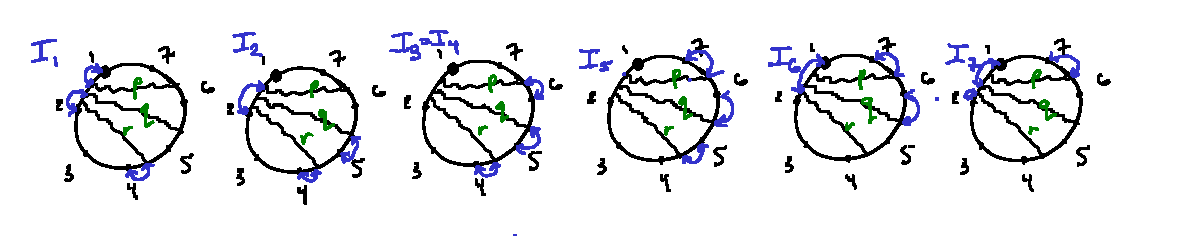
\includegraphics{egWLD_forR}
\caption{Example WLD for illustrating Algorithm~\ref{alg WLD to denom via GN} and bijections between propagators and vertices for each Grassmann necklace element.}\label{fig R eg}
\end{figure}

\begin{eg}
Consider the Wilson loop diagram in Figure~\ref{fig R eg}. Assigning propagators $p$, $q$, $s$\todo{$s = r$ in pictures} to rows $1,2,3$ respectively, we obtain the matrix
\[
C(W) = \begin{bmatrix} a & b & 0 & 0 & 0 & c & d \\ e & f & 0 & 0 & g & h & 0 \\ i & j & 0 & k & l & 0 & 0 \end{bmatrix}
\]
The Grassmann necklace of this diagram is 
\begin{gather*}I_1 = \{1,2,4\}, I_2 = \{2,4,5\}, I_3 = \{4,5,6\}, I_4=\{4,5,6\},\\ I_5=\{5,6,7\}, I_6 = \{6,7,1\}, I_7=\{7,1,2\}. \end{gather*}  
Figure~\ref{fig R eg} indicates the pairings between propagators and vertices for each $i \in [1,7]$.  

From $I_1$ to $I_2$, the propagators $p$ and $q$ change \hlfix{which vertex they are assigned to}{Can we change this language to which vertices they contribute?}. That is $I_1(p) = 1$, $I_1(q)= 2$ while $I_2(p) = 2$, $I_2(q)= 5$. However, $r$ contributes  4 to both $I_1$ and $I_2$, so $S_2 = \{p,q\}$.  Then
\[
\Delta_{I_2}=\det\begin{bmatrix} b & 0 & 0 \\ f & 0 & g \\ j & k & l \end{bmatrix} = kgb, \qquad r_2 = \det\begin{bmatrix} b & 0 & 0 \\ f & 0 & g \\ 1 & 1 & 1 \end{bmatrix} = gb.
\] {\color{violet} shouldn't $r_2$ be a $2 \times 2$ matrix? i.e. $r_2 = \det\begin{bmatrix} b & 0 \\ f &  g \end{bmatrix} = gb.$}
\hlfix{where the 1s in the third row of the second matrix correspond to the fact that $I_1(s) = I_2(s)$.}{This doesn't seem to match with what is said in the algorithm.}  Continuing likewise, we get $r_3 = c$, $r_4=1$ (since $I_4 = I_3$), $r_5 = lhd$, and $r_6 = i$.

At $I_7$ the situation \hlfix{is more complicated}{It seems to be exactly what we expect from the alg?}: we have $S_7 = \{q,s\}$ with $I_7(S_7) = \{ 1,2\}$, $\Delta_{I_7} = d(ej-fi)$ and $r_7 = ej-fi$. 

Note that unlike the previous $r_i$, $r_7$ an irriducible quadratic factor. This corresponds to the fact that $q$ and $s$ share an edge {\em and} contribute both endpoints of that edge to $I_7$; see Proposition~\ref{prop alg gives rad} below.  

Finally, we have $r_1 = (af-be)k$.  Putting everything together, we obtain
\[
R = (af-be)kgbclhdi(ej-fi)
\]
which is squarefree and contains all factors of $\prod_{i=1}^{n}\Delta_{I_i}$. If one were to construct the denominator $R(W)$ associated to this Wilson loop diagram as per Definition~\ref{def R(W)}, we would find that we have $R(W) = R$.
\end{eg}

We are now ready to begin proving the main result of this section. We begin with a proposition stating several facts about $\Delta_{I_i}$ and their relationship to $r_i$.

\begin{prop}\label{prop alg gives rad}
  With notation as in Algorithm~\ref{alg WLD to denom via GN} we have the following:
  \begin{enumerate}
    \item Each $\Delta_{I_i}$ is homogeneous, as is each $r_i$.
    \item Each $\Delta_{I_i}$ splits into linear and quadratic factors.  All linear factors of  $\Delta_{I_i}$ are single variables and all irreducible quadratic factors are $2\times 2$ determinants of single variables.
    \item Quadratic factors in $\Delta_{I_i}$ arise precisely when propagators $p$ and $q$ are supported on a common edge $(a,b)$ with $I_i(p)=a$ and $I_i(q)=b$.
    \item $r_i$ divides $\Delta_{I_i}$.
    \item The ideal generated by $R$ is the radical of the ideal generated by $\prod_{i=1}^{n}\Delta_{I_i}$.
  \end{enumerate}
\end{prop}

\begin{proof}
\begin{enumerate}
    \item The nonzero entries of $C(W)$ are independent indeterminates and so every $i\times i$ minor of $C(W)$ is either homogeneous of degree $i$ or is $0$.  Thus each $\Delta_{I_i}$ and each $r_i$ is homogeneous.  %Furthermore, each row contributes one factor to each term in the expansion of $\Delta_{I_i}$ so the result of setting the variables from a subset of rows to $1$ is still homogeneous.  Thus each $r_i$ is homogeneous.
    \item Using the expression for the determinant as a sum over permutations from Corollary~\ref{lem basis as perm} we see that $\Delta_{I_i}$ is a sum over bijections between $I_i$ and $\mathcal{P}$.  The nonzero terms in this sum are precisely those bijections such that each propagator is associated to one of its supporting vertices in $I_i$, since only those locations in $C(W)$ are nonzero.  Since the nonzero entries of $C(W)$ are independent there can be no cancellation between terms in this expansion.

Suppose $\Delta_{I_i}$ has an irreducible factor $f$.  Let $\mathcal{P}'$ be the set of propagators which contribute a variable to $f$ and let $J$ be the set of vertices which contribute a variable to $f$.

The first claim is that the minor of $C(W)$ associated to $\mathcal{P}'$ and $J$ is precisely $f$.

{\em Proof of claim}: By the structure of determinants we know that $\Delta_{I_i} = fg$, where $g$ involves only variables associated to propagators not in $\mathcal{P}'$ and associated to vertices not in $J$.  \todo{Is the heart of this proof due to the fact that there are no cancelations? It feels tautological to me, but I'm clearly not following}

Expanding out $fg$ yields a signed sum of monomials. \hlfix{In each of these monomials, $f$ contributes those variables associated both to a propagator in $\mathcal{P}'$ and to a vertex in $J$, and $g$ contributes those variables associated both to a propagator not in $\mathcal{P}'$ and to a vertex not in $J$, and no other variables appear.  }{Isn't this redundant with the previous paragraph?}


Since there is no cancellation between terms, this means that the full expansion over permutations of $\Delta_{I_i}$ contains no other nonzero terms and hence no other variables.  Therefore $\Delta_{I_i}$ is equal to the determinant of the matrix obtained by taking the submatrix of $C(W)$ with columns indexed by $I_i$ and setting any variables not appearing in $\Delta_{I_i}$ to $0$.  This new matrix is, up to permutations of rows and columns, a block matrix with one block for $\mathcal{P}'$ and $J$ and the other block for the complements.  Thus its determinant, and hence also $\Delta_{I_i}$, is the product of the minors for these two blocks.  By considering which variables appear, these two factors must also be $f$ and $g$, and so in particular $f$ is the minor of $C(W)$ associated to $\mathcal{P}'$ and $J$.  This proves the claim.

A consequence of this claim is that every linear factor of $\Delta_{I_i}$ is a $1\times 1$ minor of $C(W)$, hence is a single variable, and every irreducible quadratic factor of $\Delta_{I_i}$ is a $2\times 2$ minor of $C(W)$, hence is a $2\times 2$ determinant of single variables.

All that remains is to prove that $\Delta_{I_i}$ has no irreducible factors of degree 3 or more.  Suppose for a contradiction that $f$ is a factor of $\Delta_{I_i}$ of degree $\geq 3$. Note that by removing the propagators which come \hlfix{before}{ordering?} those contributing to $f$ and \hlfix{changing $i$ to be the first vertex}{does this generalize to other $i$?} which contributes to $f$, we obtain a \hlfix{different admissible diagram}{Is this just the diagram gotten by removing certain props?} for which $f$ still divides $\Delta_{I_i}$ but also $i\in I_i$ and
$i$ contributes to $f$.  Showing that this different admissible diagram gives a contradiction is sufficient, and so we may assume that $i\in I_i$ and $i$ contributes to $f$.  Finally, we can suppose that $W$ is minimal in number of propagators with the above occuring.

Let $p$ be the propagator such that $I_i(p) = i$. There are two cases to consider, depending on which edge $p$ is supported on.  These are illustrated in Figure~\ref{fig no big factors}

\begin{figure}
  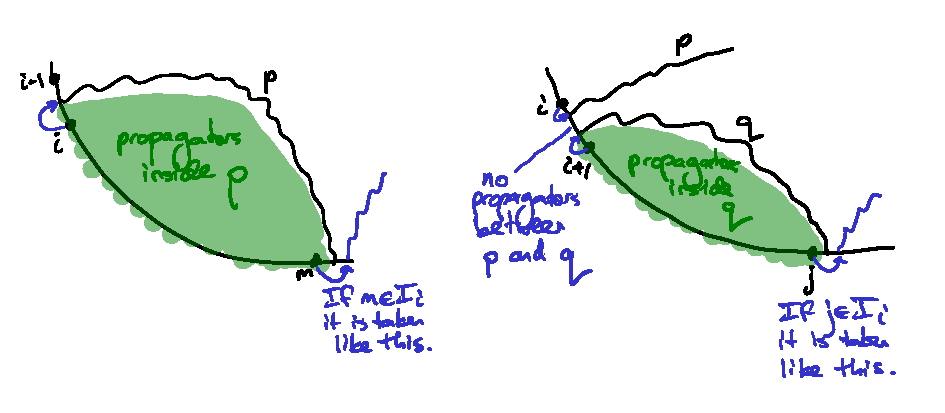
\includegraphics{no_big_factors}
  \caption{The two cases in the proof that no factors of $\Delta_{I_i}$ have degree 3 or more.}\label{fig no big factors}
\end{figure}

\textbf{Case 1}: Suppose $p$ has one end on the edge $(i-1, i)$.  Thus $p$ is supported on $(i-1, i, m, m+1)$ for some $m >_i i$, and $I_{i+1}(p) = m$ by Lemma~\ref{vertex cyclic int lem}.  

Let $S = \cP_{in}(p)$ be the set of propagators inside $p$ in the $<_i$ order. $I_i$ and $I_{i+1}$ can only differ once $p$ contributes to $I_{i+1}$, so $I_i(q) = I_{i+1}(q)$ for each $q \in S \backslash \{p\}$. Thus if a propagator contributes $m$ in $I_i$ then it must lie outside $p$.

If neither $m$ nor $m+1$ appear in $I_i$ then by Corollary~\ref{no coloops} $V(p) \cap I_i = \{i\}$, and so the row of $p$ in the matrix of $\Delta_{I_i}$ has only one nonzero entry; hence $\Delta_{I_i}$ has a linear factor contributed by $p$ and $i$, which \hlfix{is a contradiction}{Why? because $i$ contributes to $f$?}.  So we must have at least one of $m$ and $m+1$ in $I_i$.  However, all propagators in $S$ are mapped by the function $I_{i}(\cdot)$ to vertices strictly before $m$, so the matrix giving $\Delta_{I_i}$ has the form
\[
\begin{bmatrix} A & B \\ 0 & C\end{bmatrix}
\]
where $A$ is the $|S|\times |S|$ matrix indexed by the propagators in $S$ and the vertices in $I_i(S)$. No other propagators can be supported on these vertices since all other propagators are outside of $p$, and $p$ is the first propagator supported at $i$; this explains the zero block.  Therefore $\Delta_{I_i} = \det A \det C$, and both factors are nontrivial since at least one of $m$ and $m+1$ appear in $I_i$.  If we remove the propagator outside of $p$ that contributes $m$ or $m+1$, we get a smaller diagram for which $\Delta_{I_i} = \det A$ {\color{violet}why not $\det A \det C'$ with $C'$a minor of $C$?}. This contradicts the minimality of our choices unless $\det A$ is quadratic, which in turn contradicts our assumption that $i$ and $p$ contribute to an irreducible factor $f$ of degree at least 3.

\textbf{Case 2}: Suppose $p$ has one end on the edge $(i, i+1)$.  If no other propagators are supported on $i$ then the column of $C(W)$ corresponding to vertex $i$ has only one nonzero entry in it, and so $\Delta_{I_i}$ has a linear factor contributed by $p$ and $i$; as above, this is a contradiction.  Thus we can take $q$ to be the propagator such that $I_i(q)=i+1$. {\color{violet} How do we know this exists? Why can't we solve this by having $r$ supported on the $i-1^{th}$ edge?} We know that $q$ has one end on the edge $(i, i+1)$ and is adjacent to $p$ on that edge in the counterclockwise direction (see Figure \ref{fig no big factors}).  Write $(i, i+1, j, j+1)$ for the support of $q$.  The situation for $q$ is very similar to case 1: in particular, we have $I_{i+1}(q) = j$ by Lemma~\ref{vertex cyclic int lem} and so if $j\in I_i$ then the propagator which contributes $j$ is outside of $q$.  

Similarly to Case 1, let \st{$S$ be the set of propagators inside $q$ along with $p$ and $q$ themselves.}{\color{violet}$S = \cP_{in}(q)$ in the $<_i$ order. Note that $p \in S$.}\hlfix{Then all propagators in $S$ are mapped by $I_i(\cdot)$ to vertices strictly before $j$ and no other propagators are supported on vertices strictly before $j$.}{???}  Thus the matrix giving $\Delta_{I_i}$ has the form
\[
\begin{bmatrix} A & B \\ 0 & C\end{bmatrix}
\]
where $A$ is the submatrix indexed by the propagators in $S$ and the vertices in $I_i(S)$. Again two things can now happen.  If some vertex $j$ or larger (with respect to $>_i$) belongs to $I_i$ then $B$ and $C$ are at least one column wide, and so the block form of the matrix gives a nontrivial factorization of $\Delta_{I_i}$.  This yields a contradiction as in Case 1: either $W$ contains unnecessary propagators which contradicts our minimality assumption, or $\det A$ is quadratic which contradicts the assumption that $p$ and $i$ contribute to $f$, an irreducible factor of degree at least 3.  

On the other hand, if no vertex $\geq_i j$ is in $I_i$ then $\Delta_{I_i} = \det A$.  Looking in more detail into $A$, note that the only vertices in the support of $p$ and $q$ which belong to $I_i$ are $i$ and $i+1$, and hence
\[
A = \begin{bmatrix} D & 0 \\ E & F\end{bmatrix}
\]
where $D$ is the $2\times 2$ matrix indexed by the propagators $p$ and $q$ and the vertices $i$ and $i+1$.  Thus $p$ and $i$ contribute to a quadratic factor of $\Delta_{I_i}$, once again contradicting our assumptions.

All cases have now been covered and so $\Delta_{I_i}$ has only irreducible factors of degree $2$ or less.

\item Suppose propagators $p$ and $q$ are supported on a common edge $(a,b)$, with $I_i(p)=a$ and $I_i(q)=b$.  Let $x_{p,a},x_{p,b},x_{q,a},x_{q,b}$ be the associated variables in $C(W)$. For any fixed bijection $\sigma$ from $\cP-\{p,q\}$ to $I_i -\{a,b\}$ for which each propagator is supported on its image under the bijection, we can extend $\sigma$ to a bijection of all propagators with $I_i$ in two ways: either $p\mapsto a$ and $q\mapsto b$ or $p\mapsto b$ and $q\mapsto a$.  The sum of the contributions of all these bijections to $\Delta_{I_i}$ is therefore the product of \hlfix{$x_{p,a}x_{q,b}-x_{p,b}x_{q,a}$}{why? terms in determinant come from bijections. Why should all bijections appear in det?} with the minor coming from $\cP-\{p, q\}$ and $I_i - \{a,b\}$.  Since there is no cancellation of terms in the expansion of $\Delta_{I_i}$, if any other terms appear then they will cause a factor which is not in the form described in the previous part.  Therefore no such terms exist and $x_{p,a}x_{q,b}-x_{p,b}x_{q,a}$ is a factor of $\Delta_{I_i}$.

Now let $f$ be a quadratic factor of $\Delta_{I_i}$.  By part (2) we know that $f$ is a $2\times 2$ minor coming from two propagators, call them $p$ and $q$, and two vertices, call them $a <_i b$.  It remains to show that $a$ and $b$ are adjacent.  From this we can conclude that $p$ and $q$ each have one end on $(a,b)$, as any other way for both $p$ and $q$ to be supported on two consecutive vertices would contradict noncrossing or the density requirement of admissibility.

As in the proof of part (2), make a new admissible diagram by removing the propagators which come before $f$ and set $i=a$.  The cases in the proof of part (2) show how $\Delta_{I_i}$ factors: in particular the vertices supporting the other end of $p$ either do not appear in $I_i$, or they contribute to a different factor of $\Delta_{I_i}$ than $p$ and $a$ do.  By assumption $b$ contributes to the same factor as $a$.  Therefore $(a,b)$ is an edge.

\item Consider $p\in S_i$, and note that $\Delta_{I_i}$ is homogeneous linear in the variables of the row corresponding to $p$.  By part (2), either exactly one variable in the row corresponding to $p$ appears in $\Delta_{I_i}$ and this variable is a factor of $\Delta_{I_i}$, or exactly two variables from the row corresponding to $p$ appear in $\Delta_{I_i}$ and they appear as part of a quadratic factor.  In the first case let the variable be $x$. Then $x$ is a factor of $\Delta_{I_i}$ and so in particular the monomial in $\Delta_{I_i}$ corresponding to the bijection between propagators and vertices of $I_i$ associates the column of $x$ to $p$.  Thus $x$ also appears in $r_i$ and since the matrix for $r_i$ is a minor of the matrix for $\Delta_{I_i}$ and every term in $\Delta_{I_i}$ involves $x$, we also have that every term in $r_i$ involves $x$ so $x$ is a factor of both $r_i$ and $\Delta_{I_i}$ and is the only variable from this row in either polynomial.  

Now suppose two variables from the row $p$ appear in a quadratic factor $f$.  By part (3), there is another propagator $q$ and an edge $(a,b)$ such that $f$ is the $2\times 2$ minor coming from $p, q$ and $a, b$, with $I_i(p)=a$, $I_i(q)=b$.  There are two situations which can occur, both illustrated in Figure~\ref{fig quadratic}; we show that in both cases it follows that $q \in S_i$ as well.

\begin{figure}
  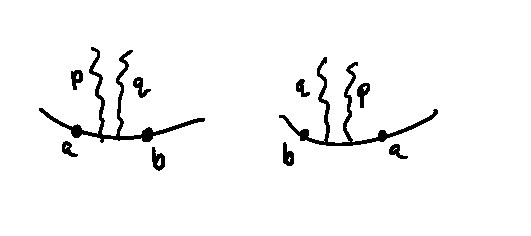
\includegraphics{quadratic}
  \caption{The situations giving a quadratic factor with variables appearing in $r_i$.}\label{fig quadratic}
\end{figure}

In both cases, since $I_{i-1}(p)\neq a$ by assumption it follows from Lemma~\ref{vertex cyclic int lem} that $I_{i-1}(p) <_{i-1} a$ and no other vertex supporting $p$ lies between $I_{i-1}(p)$ and $a$. In the case that $b<_i a$ and $q$ is assigned before $p$ in $I_i$, this means that $I_{i-1}(p)=b$ and so $I_{i-1}(q)\neq b$.  Thus $q\in S_i$ and so $f$ is a factor of $r_i$.

Now consider the case where $a<_i b$, and suppose for contradiction that $q \not\in S_i$, i.e. that $I_{i-1}(q) = b$. Since $I_{i-1}(p) \neq a$, there must be some other propagator $s$ with $I_{i-1}(s) = a$ (else $I_{i-1}$ assigns $q$ to $a$). This propagator cannot lie on edge $(a,b)$ since by Lemma~\ref{vertex cyclic int lem} we must have $I_i(s) = a$ or $b$, contradicting the fact that $I_i(p) = a$ and $I_i(q) = b$; thus $s$ has an end on $(a-1,a)$ and is inside $p$ from the point of view of $i-1$.

Say $s$ is supported on $(j, j+1, a-1, a)$ and $p$ is supported on $(k, k+1, a, b)$ with $i-1 \leq_{i-1} k+1 \leq_{i-1} j+1$. But by Lemma~\ref{lem no fourth vertex}, if $I_{i-1}(s) = a$ then $a$ cannot be maximal in the support of $s$ with respect to $<_{i-1}$; thus we must have $i-1 = j+1$, and we are in the situation in figure~\ref{fig part 4}.

\begin{figure}
  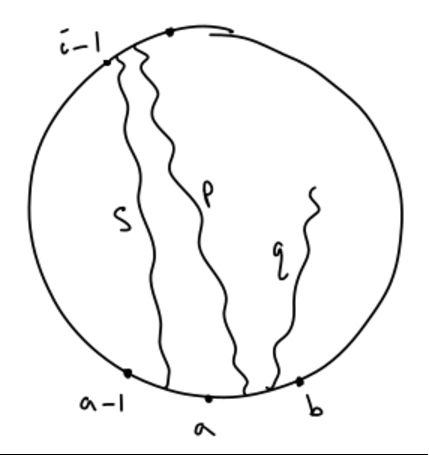
\includegraphics[scale=0.5]{part4}
  \caption{In order to obtain $I_{i-1}(s) = a$, propagators $s$ and $p$ must each have an end on the edge $(i-2,i-1)$.}\label{fig part 4}
\end{figure}

Since $p$ changed its association from $I_{i-1}$ to $I_i$, we have $I_{i-1}(p) = i-1$ by Lemma~\ref{vertex cyclic int lem}. From figure~\ref{fig part 4} it follows that $I_{i-1}$ assigns $p$ to $i-1$ and then proceeds identically to $I_i$ for all vertices inside $p$, implying that $I_{i-1}(s) = I_i(s)$. Since $I_{i-1}(s) = a$ and $I_i(s) \neq a$, this is a contradiction. 

Thus $q\in S_i$ after all, and so $f$ is a factor of $r_i$ as required.

  

% Thus $s$ is supported on $a$ but does not have an edge on $(a,b)$ and so $s$ must have an end on $(a-1, a)$ and so be inside $p$ from the point of view of $i-1$.  Say $s$ is supported on $(j, j+1, a-1, a)$ and $p$ is supported on $(k, k+1, a, b)$ with $i-1 \leq_{i-1} k+1 \leq_{i-1} j+1$.  Again by Lemma~\ref{lem susama}, immediately after $s$ contributes $a$ it must contribute $j$ and so $I_i(s)=j$.

% Finally we want to show $I_i(s)=j$ gives a contradiction.  If $k=j$ then $I_{i}(s)= k$, but $p$ has not yet been taken as $I_i(p)=a$ and $p$ comes before $s$ around $k$, so this is a contradiction.  If $k+1=j$ then similarly $I_{i}(s)=k+1$ and yet $p$ comes before $s$ around $k$, a contradiction to $I_i(p)=a$.  Now suppose $k+1 <_{i-1} j$ then we have $i-1 \leq_{i-1} k+1 <_{i-1} I_i(s) = j$ so $i\leq_{i} I_i(s)$ which gives that
% \[
% I_i(s) <_i I_{i-1}(s) \qquad \text{and} \qquad I_i(s) <_{i-1} I_{i-1}(s)
% \]
% \note{Is this known to be impossible by the proof sketch of Lemma~\ref{lem susama} that you emailed or something similar.  I'm thinking this proof is already too long and the fact that this is impossible would be better as a lemma.}

\item If $W$ has zero propagators then all $I_i=\emptyset$ and both $R$ and $\prod_{i=1}^n \Delta_{I_i}$ are equal to $1$, so the result holds in this case.  Now assume $W$ has at least one propagator.

First we show that every factor of $\prod_{i=1}^n \Delta_{I_i}$ divides $R$.  Take an irreducible factor $f$ of $\prod_{i=1}^n \Delta_{I_i}$. There exists some $i$ such that $f|\Delta_{I_i}$ but $f\!\!\nmid\!\! \Delta_{I_{i-1}}$, since otherwise the variables corresponding to the propagators contributing to $f$ which do not themselves appear in $f$ could never appear, contradicting Lemma~\ref{vertex cyclic int lem}.  If $f$ is a linear factor, say from associating propagator $p$ to vertex $a$, then $I_{i}(p)=a$ and $I_{i-1}(p)\neq a$ so this factor appears in $r_i$.  If $f$ is a quadratic factor, say from associating propagators $p$ and $q$ to vertices $a$ and $b$ respectively, then again we cannot have both $I_{i-1}(p) = a$ and $I_{i-1}(q) = b$, else $f$ divides $\Delta_{i-1}$. However, by the proof of part (4), if one of $p,q$ belongs to $S_i$ then the other does as well.  Thus $f$ divides $r_i$.

Next we need to show that $R$ is squarefree.  Suppose $f^2|R$.  If $f$ is a linear factor, say from associating propagator $p$ to vertex $a$, then there must be two distinct points in the Grassmann necklace algorithm where $p$ changes from not being associated to vertex $a$ to being associated to vertex $a$.  This contradicts Lemma~\ref{vertex cyclic int lem}.  Now suppose $f$ is a quadratic factor, say from propagators $p$ and $q$ supported on the edge $(a, b)$ with $p$ before $q$ on the edge.  In this case it is not possible for any $I_i$ to associate $p$ to $b$ and $q$ to $a$.  Furthermore, we know by part (4) that $p$ changes from not being associated to $a$ to being associated to $a$ if and only if $q$ changes from not being associated to $b$ to being associated to $b$.  Thus $f^2|R$ implies that twice in the Grassmann necklace $p$ must change from not being associated to vertex $a$ to being associated to vertex $a$. This is again a contradiction, and so $R$ is squarefree.

Taking everything together we have that $R|\prod_{i=1}^n \Delta_{I_i}$, $R$ contains all factors of $\prod_{i=1}^n \Delta_{I_i}$ and $R$ is squarefree.  Therefore the ideal generated by $R$ is the radical of the ideal generated by $\prod_{i=1}^n \Delta_{I_i}$.
  \end{enumerate}
\end{proof}


\begin{thm}\label{thm denom}
  Given any admissible Wilson loop diagram $W$, let $\{I_1, \ldots I_n\}$ be the associated Grasmann necklace. Then the denominator of the integral, $R(W)$ (see Definition~\ref{def R(W)}), is the $R$ of Algorithm~\ref{alg WLD to denom via GN}. Furthermore, the ideal generated by $R(W)$ is the radical of the ideal generated by $\prod_{i=1}^n \Delta_{I_i}$, where $\Delta_{I_i}$ is the determinant of the $k \times k$ minor indicated by $I_i$.  
\end{thm}

{\color{violet} Got rid of need for scalar multiples by talking about radicals.}

\begin{proof}
The equivalence up to scalar multiple of $R$ and the radical of $\prod_{i=1}^n \Delta_{I_i}$ is due to Proposition~\ref{prop alg gives rad}.  It remains to prove that $R(W)$ is the $R$ of Algorithm~\ref{alg WLD to denom via GN}.

To this end, first note that $R(W)$ and $R$ both have total degree $4|\mathcal{P}|$; the degree of $R(W)$ is immediate from the definition while that of $R$ follows from Lemma~\ref{vertex cyclic int lem}.  By Proposition~\ref{prop alg gives rad} every factor of $R$ is either a single variable or a quadratic factor coming from two propagators supported on a common edge.  The factors of each $R_e$ making up $R(W)$ in the notation of Definition~\ref{def R(W)} are all of this form and hence every factor of $R$ divides $R(W)$.
Finally, since $R$ is squarefree, this implies that $R(W)$ is a scalar multiple of $R$.

Finally then we need to check the scalar.  By Definition~\ref{def R(W)} each linear factor appears with coefficient $1$ and each $2\times 2$ deteriminant factor appears with the same sign as the determinant of the corresponding minor in $C(W)$.  Therefore $R=R(W)$. \todo{I'm pretty sure that there isn't a sign issue here. But do we have a proof?}
\end{proof}

Thus we have shown a deep relationship between the physically derived poles of the integrals $I(W)$ and the geometry and combinatorics associated to the diagrams $W$. At the very least, this is yet another piece of circumstantial evidence indicating that the positroid representation of Wilson loop diagrams is the correct geometric object to be considering when considering the Wilson loop amplitudes geometrically. 

While the authors cannot yet offer a proof that the appropriate sum of the Wilson loop diagrams are, in fact, finite, as conjectured [cite], we do hope that this relationship to the Grassmann Necklace elements will provide a different avenue for answering that and related questions. 


\bibliographystyle{abbrv}
\bibliography{WLDbib}

% \begin{thebibliography}{10}
% \bibitem{Adamo:2011pv}
% Tim Adamo, Mathew Bullimore, Lionel Mason, and David Skinner.
% \newblock {Scattering Amplitudes and Wilson Loops in Twistor Space}.
% \newblock {\em J.Phys.A}, A44:454008, 2011.

% \bibitem{Adamo:2012xe}
% Tim Adamo and Lionel Mason.
% \newblock {Twistor-strings and gravity tree amplitudes}.
% \newblock {\em Class.Quant.Grav.}, 30:075020, 2013.

% \bibitem{wilsonloop}
% Susama Agarwala and Eloi~Marin Amat.
% \newblock Wilson loop diagrams and positroids.
% \newblock {\em Communications in Mathematical Physics}, 2016.
% \newblock arXiv:1509.06150.

% \bibitem{casestudy}
% Susama Agarwala and Sian Fryer.
% \newblock A study in $\textrm{Gr}_{\geq 0}(2,6)$: from the geometric case book
%   of {W}ilson loop diagrams and {SYM} $n=4$.
% \newblock arXiv:1803.00958.

% \bibitem{non-orientable}
% Susama Agarwala and Cameron Marcott.
% \newblock Wilson loops in sym $n=4$ do not parametrize an orientable space.
% \newblock arXiv:1807.05397.

% \bibitem{UnwindingAmplituhedron}
% Nima Arkani-Hamed, Hugh Thomas, and Jaroslav Trnka.
% \newblock Unwinding the amplituhedron in binary.
% \newblock {\em Journal of High Energy Physics}, 2018(1):16, Jan 2018.
% \newblock arXiv:1704.05069.

% \bibitem{Arkani-Hamed:2013kca}
% Nima Arkani-Hamed and Jaroslav Trnka.
% \newblock {Into the Amplituhedron}.
% \newblock {\em JHEP}, 12:182, 2014.

% \bibitem{Arkani-Hamed:2013jha}
% Nima Arkani-Hamed and Jaroslav Trnka.
% \newblock {The Amplituhedron}.
% \newblock {\em JHEP}, 10:30, 2014.

% \bibitem{Boels:2007qn}
% Rutger Boels, Lionel Mason, and David Skinner.
% \newblock {From twistor actions to MHV diagrams}.
% \newblock {\em Phys.Lett.}, B648:90--96, 2007.

% \bibitem{Bullimore:2010pj}
% Mathew Bullimore, Lionel Mason, and David Skinner.
% \newblock {MHV Diagrams in Momentum Twistor Space}.
% \newblock {\em JHEP}, 1012:032, 2010.

% \bibitem{CasteelsPaths}
% K. Casteels.
% \newblock Quantum matrices by paths.
% \newblock {\em Algebra Number Theory}, 8(8):1857--1912, 2014.

% \bibitem{Amplituhedronsquared}
% Burkhard Eden, Paul Heslop, and Lionel Mason.
% \newblock The AmplituhedronSquared.
% \newblock 2017.
% \newblock arxiv:1701.00453.

% \bibitem{galashinlam}
% P.~{Galashin} and T.~{Lam}.
% \newblock {Parity duality for the amplituhedron}.
% \newblock {\em arXiv e-prints}, May 2018.

% \bibitem{HeslopStewart}
% Paul Heslop and Alastair Stewart.
% \newblock The twistor wilson loop and the amplituhedron.
% \newblock {\em Journal of High Energy Physics}, 2018(10):142, Oct 2018.

% \bibitem{Hodges:2012ym}
% Andrew Hodges.
% \newblock {A simple formula for gravitational MHV amplitudes}.
% \newblock 2012.

% \bibitem{AmplituhedronDecomposition}
% Steven~N. Karp, Lauren~K. Williams, and Yan~X. Zhang.
% \newblock Decompostions of amplituhedra.
% \newblock arXiv:1708.09525.

% \bibitem{GrassmannAmplitudebook}
% Freddy Cachazo Alexander Goncharov Alexander Postnikov Jaroslav~Trnka
%   Nima~{A}rkani {H}amed, Jacob~Bourjaily.
% \newblock {\em Grassmannian Geometry of Scattering Amplitudes}.
% \newblock Cambridge University Press, Cambridge, UK, 2016.

% \bibitem{LipsteinMason}
% Arthur E. Lipstein, Lionel Mason
% \newblock From dlogs to dilogs; the super Yang-Mills MHV amplitude revisited
% \newblock J. High Energ. Phys. (2014) 2014: 169.

% \bibitem{reversingOh}
% S. Agarwala, S. Fryer.
% \newblock An algorithm to construct the Le diagram associated to a Grassmann necklace
% \newblock \url{arXiv:1803.01726}

% \bibitem{Gale}
% D. Gale.
% \newblock Optimal assignments in an ordered set: {A}n application of matroid theory.
% \newblock {\em J. Combinatorial Theory}, 4: 176 - 180 (1968).

% \bibitem{Oh}
% S. Oh.
% \newblock Positroids and {S}chubert matroids.
% \newblock {\em J. Combin. Theory Ser. A}, 118(8):2426--2435, (2011)

% \bibitem{Oh2}
%   S. Oh.
%   \newblock Combinatorics of positroids.
%   \newblock {\em DMTCS Proceedings vol. AK},(FPSAC 2009), 721--732

% \bibitem{Postnikov}
% A.~Postnikov.
% \newblock Total positivity, {G}rassmannians, and networks.
% \newblock \url{arXiv:math/0609764}.


% \end{thebibliography}

\end{document}
